%\documentclass[acmsmall,review]{acmart}
\documentclass[acmsmall, screen]{acmart}
%\settopmatter{printfolios=true,printccs=false,printacmref=false}

\startPage{1}

\bibliographystyle{ACM-Reference-Format}
\citestyle{acmauthoryear}   %% For author/year citations

\usepackage{booktabs}   %% For formal tables:
                        %% http://ctan.org/pkg/booktabs
\usepackage{subcaption} %% For complex figures with subfigures/subcaptions
                        %% http://ctan.org/pkg/subcaption

\usepackage{algorithm}% http://ctan.org/pkg/algorithms
\usepackage{algpseudocode}% http://ctan.org/pkg/algorithmicx

\usepackage{boldline,multirow}

\usepackage{makecell, multirow}
\usepackage[inline]{enumitem}
\usepackage{listings}
\usepackage{graphicx}
\usepackage{color}

\usepackage{tabulary} \usepackage{tabularx}

\usepackage{tikz} \usetikzlibrary{shapes,arrows,positioning}
\usepackage{multicol}

\usepackage{proof}

\usepackage{caption}
% \usepackage{subcaption}
\definecolor{dkgreen}{rgb}{0,0.6,0}
\definecolor{gray}{rgb}{0.5,0.5,0.5}
\definecolor{mauve}{rgb}{0.58,0,0.82}

\lstset{ language=Java, aboveskip=3mm, belowskip=3mm,
  showstringspaces=false, columns=flexible,
  basicstyle={\small\ttfamily}, numbers=left, numbersep=5pt,
  numberstyle=\small\color{gray}, keywordstyle=\color{blue},
  commentstyle=\color{dkgreen}, stringstyle=\color{mauve},
  breaklines=true, breakatwhitespace=true, tabsize=3 }

% \tikzstyle{block} = [rectangle, draw, fill=white, text width=5em,
% text centered, rounded corners, minimum height=4em]
\tikzstyle{block} = [rectangle, draw, fill=white, text width=3em, text
centered, rounded corners, minimum height=3em] 
\tikzstyle{block2} =
[rectangle, draw, fill=white, text width=5em, text centered, rounded
corners, minimum height=3em] \tikzstyle{line} = [draw, -latex']
\setcopyright{rightsretained}





\begin{document}

% %% Title information
% \title[Short Title]{Full Title} %% [Short Title] is optional;
%                                         %% when present, will be
%                                         %% used in
%                                         %% header instead of Full
%                                         %% Title.
% \titlenote{with title note} %% \titlenote is optional;
%                                         %% can be repeated if
%                                         %% necessary;
%                                         %% contents suppressed with
%                                         %% 'anonymous'
% \subtitle{Subtitle} %% \subtitle is optional
% \subtitlenote{with subtitle note} %% \subtitlenote is optional;
%                                         %% can be repeated if
%                                         %% necessary;
%                                         %% contents suppressed with
%                                         %% 'anonymous'


% \title{Context Tunneling for Points-to Analysis}
% \subtitle{Maximizing the Potential of $k$-Context-Sensitivity with
% Data-Driven Optimization}
\title{Precise and Scalable Points-to Analysis via Data-Driven Context
  Tunneling}

\author{Minseok Jeon}
\email{minseok_jeon@korea.ac.kr} %% \email is recommended
\affiliation{
	% \position{Student}
	\department{Department of Computer Science and
		Engineering} %% \department is recommended
	\institution{Korea University} %% \institution is required
	\streetaddress{145, Anam-ro} \city{Sungbuk-gu} \state{Seoul}
	\postcode{02841} \country{Republic of Korea} }
\author{Sehun Jeong} \email{gifaranga@korea.ac.kr}
\affiliation{
	% \position{Student}
	\department{Department of Computer Science and
		Engineering} %% \department is recommended
	\institution{Korea University} %% \institution is required
	\streetaddress{145, Anam-ro} \city{Sungbuk-gu} \state{Seoul}
	\postcode{02841} \country{Republic of Korea} }
\author{Hakjoo Oh}
\authornote{Corresponding author}
\email{hakjoo_oh@korea.ac.kr} %% \email is recommended
\affiliation{
  % \position{Student}
  \department{Department of Computer Science and
    Engineering} %% \department is recommended
  \institution{Korea University} %% \institution is required
  \streetaddress{145, Anam-ro} \city{Sungbuk-gu} \state{Seoul}
  \postcode{02841} \country{Republic of Korea} }


\begin{CCSXML}
	<ccs2012>
	<concept>
	<concept_id>10003752.10010124.10010138.10010143</concept_id>
	<concept_desc>Theory of computation~Program analysis</concept_desc>
	<concept_significance>500</concept_significance>
	</concept>
	<concept>
	<concept_id>10010147.10010257.10010293</concept_id>
	<concept_desc>Computing methodologies~Machine learning approaches</concept_desc>
	<concept_significance>500</concept_significance>
	</concept>
	</ccs2012>
\end{CCSXML}

\ccsdesc[500]{Theory of computation~Program analysis}
\ccsdesc[500]{Computing methodologies~Machine learning approaches}

%%% The following is specific to OOPSLA '18 and the paper
%%% 'Precise and Scalable Points-to Analysis via Data-Driven Context Tunneling'
%%% by Minseok Jeon, Sehun Jeong, and Hakjoo Oh.
%%%
\acmPrice{}
\acmDOI{10.1145/3276510}
\acmYear{2018}
\copyrightyear{2018}
\acmJournal{PACMPL}
\acmVolume{2}
\acmNumber{OOPSLA}
\acmArticle{140}
\acmMonth{11}


%% Keywords comma separated list
\keywords{Points-to analysis, Context-sensitive analysis, Data-driven
  program
  analysis} %% \keywords are mandatory in final camera-ready submission

\newcommand{\mca}{\mathcal{A}}
\newcommand{\mcb}{\mathcal{B}}
\newcommand{\mcc}{\mathcal{C}}
\newcommand{\mcf}{\mathcal{F}}
\newcommand{\mcg}{\mathcal{G}}
\newcommand{\mcp}{\mathcal{P}}
\newcommand{\mcl}{\mathcal{L}}
\newcommand{\mcm}{\mathcal{M}}
\newcommand{\mco}{\mathcal{O}}
\newcommand{\mcu}{\mathcal{U}}
\newcommand{\mcv}{\mathcal{V}}
\newcommand{\mcr}{\mathcal{R}}

\newcommand{\myland}{\;\land\;}
\newcommand{\mylor}{\;\vee\;}

\newcommand{\power}[1]{\wp(#1)}

\newcommand{\myset}[1]{\{ #1 \}}
\newcommand{\myvec}[1]{\langle #1 \rangle}

\newcommand{\db}[1]{\llbracket #1 \rrbracket}
\newcommand{\pdb}[1]{\llbracket #1 \rrbracket_{\pconf}}
\newcommand{\ppdb}[1]{\llbracket #1 \rrbracket^{\pre}}
\newcommand{\po}{{po}}




%%%%Tunneling


%% Learning
\newcommand{\Classifier}{\mathcal{C}}
%\newcommand{\argmax}[1]{\underset{#1}{\mathrm{argmax}}}
\newcommand{\argmax}{\operatornamewithlimits{argmax}}

%% Comment
\newcommand{\todoc}[2]{{\textcolor{#1} {\textbf{[[#2]]}}}}

\newcommand{\todored}[1]{\todoc{red}{#1}}
\newcommand{\todoblue}[1]{\todoc{blue}{#1}}
\newcommand{\todogreen}[1]{\todoc{green}{#1}}

\newcommand*{\TODO}[1]{\todored{#1}}
\newcommand*{\minseok}[1]{\todoblue{Minseok: #1}}
\newcommand{\commentout}[1]{}

\newcommand{\abst}{}
\newcommand{\aF}{\abst{F}}
\newcommand{\oracle}{{\mathcal{O}}}
\newcommand{\floor}[1]{\lfloor #1 \rfloor}
%% Program
\newcommand{\mba}{\mathbb{A}}
\newcommand{\mbb}{\mathbb{B}}
\newcommand{\mbc}{\mathbb{C}}
\newcommand{\mbd}{\mathbb{D}}
\newcommand{\mbe}{\mathbb{E}}
\newcommand{\mbf}{\mathbb{F}}
\newcommand{\mbg}{\mathbb{G}}
\newcommand{\mbh}{\mathbb{H}}
\newcommand{\mbi}{\mathbb{I}}
\newcommand{\mbj}{\mathbb{J}}
\newcommand{\mbk}{\mathbb{K}}
\newcommand{\mbl}{\mathbb{L}}
\newcommand{\mbm}{\mathbb{M}}
\newcommand{\mbn}{\mathbb{N}}
\newcommand{\mbo}{\mathbb{O}}
\newcommand{\mbp}{\mathbb{P}}
\newcommand{\mbq}{\mathbb{Q}}
\newcommand{\mbr}{\mathbb{R}}
\newcommand{\mbs}{\mathbb{S}}
\newcommand{\mbt}{\mathbb{T}}
\newcommand{\mbu}{\mathbb{U}}
\newcommand{\mbv}{\mathbb{V}}
\newcommand{\mbw}{\mathbb{W}}
\newcommand{\mbx}{\mathbb{X}}
\newcommand{\mby}{\mathbb{Y}}
\newcommand{\mbz}{\mathbb{Z}}
\newcommand{\cfgto}{\hookrightarrow}

\newcommand*{\cD}{\mathcal{D}}
\newcommand*{\cF}{\mathcal{F}}
\newcommand*{\cP}{\mathcal{P}}
\newcommand*{\cV}{\mathcal{V}}

\newcommand{\mcs}{\mathcal{S}}
\newcommand{\wv}{\mathbf{w}}
\newcommand{\Pgm}{{\it Pgm}}

\newcommand{\Hint}{{\it Profile}}
\newcommand{\hint}{R}
\newcommand{\compo}{\mbj}
\newcommand{\importance}{\mbr}
\newcommand{\feat}{f}
\newcommand{\features}{{\vec{\feat}}}
\newcommand{\strategy}{\mathcal{S}}

\newcommand{\score}{{\it score}}

\newcommand{\mse}{E}

\let\oldvec\vec
\renewcommand{\vec}[1]{\mathbf{#1}}


\newcommand{\obj}{{\it obj}}
\newcommand{\model}{\mathcal{M}}
\newcommand{\counter}{\mathcal{C}}
\newcommand{\lfp}{{\sf lfp}}
\newcommand{\widenop}{\triangledown}
\newcommand{\lub}{{\it lub}}
\newcommand{\glb}{{\it glb}}

\newcommand*{\sans}{\fontfamily{phv}\selectfont}
\newcommand*{\cour}{\fontfamily{pcr}\selectfont}

\newcommand{\true}{{\it true}}
\newcommand{\false}{{\it false}}
\newcommand{\afeatures}{\mba}
\newcommand{\afeat}{a}
\newcommand{\Methods}{{\mbm}}
\newcommand{\Invos}{{\mbi}}
\newcommand{\sem}[1]{[\![#1]\!]}
\newcommand{\mthd}{{{M}}}
\newcommand{\Program}{\mbp}
\newcommand{\selector}{S}
\newcommand{\component}{\mbm}
\newcommand{\idx}{j}
\newcommand{\heuristic}{\mathcal{H}}
\newcommand{\weight}{\vec{w}}
\newcommand{\formulas}{\mcf}
\newcommand{\cost}{{\sf cost}}
\newcommand{\proved}{{\sf proved}}
\newcommand{\method}{{\sf meth}}
\newcommand{\precision}{\proved}

\newcommand{\pr}{\Psi}

\newcommand{\Assertion}{\mbq}

\newcommand{\params}{\Pi}
\newcommand{\lparams}{\Theta}
\newcommand{\lparam}{\theta}

\renewcommand{\algorithmicrequire}{\textbf{Input:}}
\renewcommand{\algorithmicensure}{\textbf{Output:}}
\newcommand{\ChooseClause}{{\sf ChooseClause}}
\newcommand{\ChooseAtom}{{\sf ChooseRefiner}}
\newcommand{\ChooseSeed}{{\sf ChooseSeed}}
\newcommand{\RefineSeed}{{\textsc{RefineSeed}}}
\newcommand{\PrecP}{{\sf Prec^{+}}}
\newcommand{\PrecE}{{\sf Prec^{=}}}
\newcommand{\CostM}{{\sf Cost^{-}}}
\newcommand{\HasSeed}{{\sf HasPotential}}
\newcommand{\GoodHeuristicFound}{{\sf BetterHeuristicFound}}
\newcommand{\isSatisfactory}{{\sf isSatisfactoryPrecision}}

\newcommand{\hypospace}{\mathcal{M}}

\newcommand{\AnalyzeWith}{{\sf Analyze}}

\newcommand{\Record}{{\sf record}}
\newcommand{\Merge}{{\sf merge}}
\newcommand{\MergeTunneled}{\textbf{\textsc{ParentContext}}}
\newcommand{\MergeStatic}{\textbf{\textsc{MergeStatic}}}
\newcommand{\ectx}{\star}
\newcommand{\ApplyDepth}{\textsc{\textbf{ApplyDepth}}}
\newcommand{\Tunnel}{\textsc{\textbf{Tunnel}}}
\newcommand{\ContextMadeIn}{{{\textsc{\textbf{ParentMethod}}}}}
\newcommand{\Tunneling}{{{\textsc{{Tunneling}}}}}
\newcommand{\TunnelingRelation}{\mathcal{T}}

\newcommand{\childMeth}{{\it childMeth}}

\newcommand{\onesobjH}{{\it S1objH}}
\newcommand{\oneobjH}{{\it 1objH}}
\newcommand{\onetypeH}{{\it 1typeH}}
\newcommand{\onecallH}{{\it 1callH}}
\newcommand{\onecall}{{\it 1call}}

\newcommand{\onesobjHT}{{\it S1objH+T}}
\newcommand{\bonesobjHT}{{\textit{\textbf{S1objH+T}}}}
\newcommand{\oneobjHT}{{\it 1objH+T}}
\newcommand{\onetypeHT}{{\it 1typeH+T}}
\newcommand{\onecallHT}{{\it 1callH+T}}

\newcommand{\twosobjH}{{\it S2objH}}
\newcommand{\threesobjH}{{\it S3obj2H}}
\newcommand{\twoobjH}{{\it 2objH}}
\newcommand{\twotypeH}{{\it 2typeH}}
\newcommand{\twocallH}{{\it 2callH}}

\newcommand{\kobjkH}{{\it kobj+kH}}

\newcommand{\sobjHdata}{{\it \sobjH+Data}}
\newcommand{\objHdata}{{\it \objH+Data}}
\newcommand{\typeHdata}{{\it \typeH+Data}}
\newcommand{\calldata}{{\it \call+Data}}

\newcommand{\sobjHIntroA}{{\it \sobjH+IntroA}}
\newcommand{\objHIntroA}{{\it \objH+IntroA}}
\newcommand{\typeHIntroA}{{\it \typeH+IntroA}}
\newcommand{\callHIntroA}{{\it \call+IntroA}}

\newcommand{\sobjHIntroB}{{\it \sobjH+IntroB}}
\newcommand{\objHIntroB}{{\it \objH+IntroB}}
\newcommand{\typeHIntroB}{{\it \typeH+IntroB}}
\newcommand{\callHIntroB}{{\it \call+IntroB}}

\newcommand{\pair}{{\it pair}}
\newcommand{\first}{{\it first}}
\newcommand{\second}{{\it second}}

\newcommand{\classof}{{\it classof}}
\newcommand{\methof}{{\it methof}}
\newcommand{\typeof}{{\it typeof}}
\newcommand{\lookup}{{\it lookup}}
%\newcommand{\methofinvo}{{\sf methof}}

\newcommand{\truncateCtx}[2]{{\lceil #1 \rceil_{#2}}}
%\newcommand{\truncateCtx}[2]{{\sf last}_{#2}(#1)}
\newcommand{\appendCtx}[2]{#1 \concat #2}

\newcommand{\ctxElem}{{\sf ctxof}}
\newcommand{\pctx}{{\it pctx}}
\newcommand{\parentCtx}{{\sf pctx}}
\newcommand{\parentMeth}{{\sf pmeth}}

\newcommand{\parentMethod}{{\sf pmeth}}

\newcommand{\hide}[1]{}

%%%%%%%%%%%%%%%%%%%%%%%%%%%%%%
%% relations for representing programs
%%%%%%%%%%%%%%%%%%%%%%%%%%%%%%

\newcommand{\meth}{{\it meth}}
\newcommand{\toMeth}{{\it m'}}
\newcommand{\inMeth}{{\it m}}

\newcommand{\ctx}{{\it ctx}}
\newcommand{\toCtx}{{\it c}_2}
\newcommand{\fromCtx}{{\it c}_1}
\newcommand{\hctx}{{\it hctx}}
\newcommand{\heap}{{\it heap}}
\newcommand{\var}{{\it x}}
\newcommand{\tovar}{{\it x}}
\newcommand{\fromvar}{{\it y}}
\newcommand{\base}{{\it z}}
\newcommand{\baseH}{{\it h}'}
\newcommand{\baseHCtx}{{\it hc}'}
\newcommand{\fld}{{\it f}}
\newcommand{\calleeCtx}{{\it c}_2}
\newcommand{\callerCtx}{{\it c}_1}
\newcommand{\invo}{{\it l}}

\newcommand{\this}{{\it this}}
\newcommand{\sig}{{\it sig}}
\newcommand{\heapT}{{\it hT}}

\newcommand{\Alloc}{\textsc{Alloc}}
\newcommand{\Move}{\textsc{Move}}
\newcommand{\Load}{\textsc{Load}}
\newcommand{\Store}{\textsc{Store}}
\newcommand{\VCall}{\textsc{Call}}
\newcommand{\SCall}{\textsc{SCall}}
\newcommand{\FormalArg}{\textsc{FormalArg}}
\newcommand{\ActualArg}{\textsc{ActualArg}}
\newcommand{\FormalReturn}{\textsc{FormalReturn}}
\newcommand{\ActualReturn}{\textsc{ActualReturn}}
\newcommand{\ThisVar}{\textsc{ThisVar}}
\newcommand{\HeapType}{\textsc{HeapType}}
\newcommand{\LookUp}{\textsc{LookUp}}

\newcommand{\VarPointsTo}{\textit{ptsto}}
\newcommand{\CallGraph}{\textit{callgraph}}
\newcommand{\FldPointsTo}{\textit{fldptsto}}
\newcommand{\InterProcAssign}{\textit{InterProcAssign}}
\newcommand{\Reachable}{\textit{reachable}}

\newcommand{\Flavor}{{\it flavor}}
\newcommand{\Flavorcall}{\Flavor_{\it call}}
\newcommand{\Flavorobj}{\Flavor_{\it obj}}
\newcommand{\Flavorsobj}{\Flavor_{\it sobj}}
\newcommand{\Flavortype}{\Flavor_{\it type}}

\newcommand{\parent}{\Flavor}
\newcommand{\parentcall}{\Flavorcall}
\newcommand{\parentsobj}{\Flavorsobj}
\newcommand{\parentobj}{\Flavorobj}
\newcommand{\parenttype}{\Flavortype}


\newcommand{\HeapDepth}{{\it maxH}}
\newcommand{\CallDepth}{{\it maxK}}


\newcommand{\concat}{%
  \mathbin{{+}\mspace{-8mu}{+}}%
}

\newcommand{\cmd}{{\it inst}}
\newcommand{\lcmd}{{\it linst}}

\newcommand{\Context}{\mbc}
\newcommand{\HeapContext}{\mbh\mbc}

\newcommand{\myparagraph}[1]{\paragraph{\fontshape{\itdefault}\fontseries{\bfdefault}\selectfont
#1\/}}

\newcommand{\Bean}{\textsc{Bean}}

\newcommand{\fprime}{f_{\it imp}}
\newcommand{\fsecond}{f_{\it unimp}}

\newcommand{\tspace}{\mcr}

\newcommand{\LearnBooleanFormula}{\textsc{LearnParameter}}
\newcommand{\CollectSeedFeatures}{\textsf{CollectSeedFeatures}}
\newcommand{\Failed}{{\it Failed}}

\newcommand{\SeedFeature}{\textsf{SeedFeature}}



%%Obj2CFA



\let\oldvec\vec
\renewcommand{\vec}[1]{\mathbf{#1}}




\renewcommand{\algorithmicrequire}{\textbf{Input:}}
\renewcommand{\algorithmicensure}{\textbf{Output:}}
\newcommand{\Update}{{\sf Update}}
\newcommand{\Prec}{{\sf Prec}}
\newcommand{\Refiner}{\Gamma}

\newcommand{\RefineClause}{{\sf RefineClause}}

\newcommand{\BetterThan}{{\sf Improved}}

\newcommand{\oneobjHTnew}{\oneobjHT$_{\it new}$}
%\newcommand{\oneobjHT}{{\it 1objH+$\objheuristic$}}

%\newcommand{\onecallHT}{{\it 1callH+$\callheuristic$}}

\newcommand{\callH}{{\it 1callH+S}}
%\newcommand{\bsimonecallH}{\textit{\textbf{1callH+S}}}
\newcommand{\sobjSimLearn}{{\it 1callH+SL'}}
\newcommand{\simonecallH}{{\it 1callH+S'}}

\newcommand{\kth}{\text{\it last}}

\newcommand{\Graphick}{{\sc Graphick}}
\newcommand{\Scaler}{{\it Scaler}}
\newcommand{\Zipper}{{\it Zipper}}
\newcommand{\twoobjZipper}{{\it 2objH+Zip}}
\newcommand{\oursZipper}{{\it 1callH+SL+Zip}}
%\newcommand{\Zipper}{{\it Zipper}}


\newcommand{\twoobjHT}{{\it 2objH+T}}
\newcommand{\ours}{{\it 1callH+SL}}
\newcommand{\oursim}{{\it 1callH+S}}
\newcommand{\oursbf}{{\it\textbf{1callH+SL}}}
%\newcommand{\ours}{{\it 1callH+$\heuristic_{\sf ours}$}}

\newcommand{\onecallThis}{{\it 1callH+T$_{C1}$}}

\newcommand{\onecallHours}{{\it 1callH+}$\heuristic_f$}
\newcommand{\onecallHdtree}{{\it 1callH+}$\heuristic$}
%\newcommand{\onecallHDT}{{\it 1callH+}$\heuristic_\decisionTree$}
\newcommand{\onecallHDT}{{\it 1callH+D}}
\newcommand{\onecallHL}{{\it 1callH+L}}


\newcommand{\threeobjH}{{\it 3obj2H}}


%%%%%%%%%%%%%%%%%%%%%%%%%%%%%%
%% relations for representing programs
%%%%%%%%%%%%%%%%%%%%%%%%%%%%%%




%\newcommand{\myparagraph}[1]{\paragraph{\fontshape{\itdefault}\fontseries{\bfdefault}\selectfont
%#1\/}}

\newcommand{\mybf}[1]{{\fontshape{\itdefault}\fontseries{\bfdefault}\selectfont#1\/}}



%\newcommand{\Simulation}{\textsc{Simulation}}
%\newcommand{\Recovery}{\textsc{Recovery}}


\newcommand{\CallGraphEdge}{{\sf CallGraphEdge}}


\newcommand{\Inst}{\text{\it Label}}
\newcommand{\Invo}{\text{\it Invo}}
\newcommand{\inst}{l}
\newcommand{\fix}{{\it fix}}
\newcommand{\entry}{\text{\it main}}
\newcommand{\emptyctx}{\epsilon}
\newcommand{\updatectx}{U}
\newcommand{\Var}{\text{\it Var}}
\newcommand{\Ctx}{\text{\it Ctx}}
\newcommand{\Heap}{\text{\it Heap}}
\newcommand{\Hctx}{\text{\it Hctx}}
\newcommand{\project}{\Pi}
\newcommand{\weakupdate}{\stackrel {{\it w}}{\mapsto}}


%\newcommand{\fld}{{\it fld}}
\newcommand{\ptsto}{X}
\newcommand{\fptsto}{Y}
\newcommand{\reachable}{R}
\newcommand{\callgraph}{G}

\newcommand{\mthdof}{\text{\it Mthdof}}

\newcommand{\moreprecise}{\succeq}
\newcommand{\strictlylessprecise}{\prec}


\newcommand{\decisionTree}{{\sf DT}}
\newcommand{\simulate}{{\sf simulate}}
\newcommand{\Tobj}{T_{\text{\it obj}}}
\newcommand{\call}{{\sf call}}
\newcommand{\Tcall}{T_{\text{\it call}}}
\newcommand{\learn}{{\sf learn}}
\newcommand{\callheuristic}{\heuristic_{\sf call}}
\newcommand{\objheuristic}{\heuristic_{\sf obj}}
\newcommand{\simheuristic}{\heuristic_{{\sf sim}}}
\newcommand{\dtheuristic}{\heuristic_{{\sf \decisionTree}}}
\newcommand{\ourheuristic}{\heuristic_{{\sf ours}}}



\newcommand{\featmean}[2]{\sem{#1}_{#2}}
\newcommand{\xor}{\oplus}

%\newcommand{\Gobj}{G_{\it obj}}
\newcommand{\Gobj}{G}
\newcommand{\transform}{{\sf transform}}

\newcommand{\objective}{{\it O}}


\newcommand{\learnold}{A}
\newcommand{\learnsup}{B}

\newcommand{\ourtechnique}{\textsc{Obj2Cfa}}



%\newcommand{\Existing}{{\it Existing}~\cite{JeJeOh18}}
\newcommand{\Existing}{{\it 1callH+T$_{\it new}$}}
\newcommand{\DecisionTree}{{\it Decision tree}}
\newcommand{\OurLearn}{{\it 1callH+SL}}

\newcommand{\failcasts}{\#may-fail-casts}

\newcommand{\callgraphedges}{\#call-graph-edges}
\newcommand{\reachableMethods}{\#reachable-methods}
\newcommand{\polycalls}{\#polymorphic-calls}



\newcommand{\ideal}{{\it ideal}}
\newcommand{\onepgm}{{\{luindex\}}}
\newcommand{\twopgm}{{\{luindex, lusearch\}}}
\newcommand{\threepgm}{{\{luindex, lusearch, antlr\}}}
\newcommand{\fourpgm}{{\{luindex, lusearch, antlr, pmd\}}}

\newcommand{\hyper}{{\theta}}

\newcommand{\Lait}{{\sc Lait}}
\newcommand{\Eagle}{\textsc{Eagle}}

\newcommand{\abs}{{\bf a}}
\newcommand{\absk}{{\bf k}}
\newcommand{\absz}{{\bf 0}}



\newcommand{\Refine}{{\textit{Refine}}}
\newcommand{\Specify}{{\textit{Specify}}}
\newcommand{\Score}{{\textit{Score}}}

\newcommand{\GraphPtsTo}{{{G_{\textit {FPG}}}}}
\newcommand{\NodePtsTo}{{{N_{\textit{FPG}}}}}
\newcommand{\EdgePtsTo}{{{\hookrightarrow_{\textit{FPG}}}}}

\newcommand{\GraphOAG}{{{G_{\textit{OAG}}}}}
\newcommand{\NodeOAG}{{{N_{\textit{OAG}}}}}
\newcommand{\EdgeOAG}{{{\hookrightarrow_{\textit{OAG}}}}}

\newcommand{\New}{{\textit{New}}}
\newcommand{\Replace}{{\textit{Replace}}}
\newcommand{\Append}{{\textit{Append}}}

\newcommand{\MaxIn}{{\textit{MaxIn}}}
\newcommand{\MaxOut}{{\textit{MaxOut}}}

\newcommand{\ourtool}{{\sc Graphick}}

\newcommand{\TypeBased}{{\it Type-Based}}
\newcommand{\AllocBased}{{\it Alloc-Based}}
\newcommand{\Mahjong}{{\sc Mahjong}}
\newcommand{\OurHeap}{\ourtool}



\newcommand{\Data}{{\sc Data}}

\newcommand{\Insens}{{\it Insens}}

\newcommand{\Doop}{{\sc Doop}}
%\newcommand{\OurCtx}{{\it 2objH+Ours}}
\newcommand{\OurCtx}{\ourtool}

\newcommand{\Principle}{{\it heuristic}}

%% Learning

%\newcommand{\argmax}[1]{\underset{#1}{\mathrm{argmax}}}


%% Comment

\newcommand*{\sehun}[1]{\todoblue{Sehun: #1}}
\newcommand*{\hakjoo}[1]{\todoblue{Hakjoo: #1}}

\newcommand*{\junhee}[1]{\todoblue{Minseok: #1}}




\let\oldvec\vec
\renewcommand{\vec}[1]{\mathbf{#1}}



\newcommand{\comp}{c}




\renewcommand{\algorithmicrequire}{\textbf{Input:}}
\renewcommand{\algorithmicensure}{\textbf{Output:}}



\newcommand{\bsimonecallH}{\textit{\textbf{1callH+S}}}

\newcommand{\twoobjHData}{{\it 2objH+Data}}


%%%%%%%%%%%%%%%%%%%%%%%%%%%%%%
%% relations for representing programs
%%%%%%%%%%%%%%%%%%%%%%%%%%%%%%


\newcommand{\heapAbstraction}{{\it HeapAbstraction}}
\newcommand{\ctxAbstraction}{{\it ContextAbstraction}}



\newcommand{\inmeth}{{\it inMeth}}
\newcommand{\calleemeth}{{\it callee}}
\newcommand{\callermeth}{{\it caller}}


\newcommand{\alloc}{{\it alloc}}
\newcommand{\type}{{\it type}}


%\newcommand{\arg}{{\it arg}}
\newcommand{\param}{{\it param}}

\newcommand{\returnvar}{{\it return}}







\newcommand{\ArrLoad}{\textit{ArrLoad}}
\newcommand{\ArrStore}{\textit{ArrStore}}


\newcommand{\ArrPointsTo}{\textit{ArrPtsTo}}

\newcommand{\MethodCtx}{\textit{MethodCtx}}

\newcommand{\Callgraph}{\textit{callgraph}}




%\newcommand{\Simulation}{\textsc{Simulation}}
%\newcommand{\Recovery}{\textsc{Recovery}}


\newcommand{\projgraph}{{\tt graph}}
\newcommand{\projproved}{{\tt proved}}
\newcommand{\projcost}{{\tt cost}}

\newcommand{\itvlst}{{\it ItvList}}
\newcommand{\itv}{{\it itv}}
\newcommand{\Itv}{{\it Itv}}

\newcommand{\feature}{f}
\newcommand{\Feature}{{\it Feature}}
\newcommand{\Feat}{\mcf}
\newcommand{\aNode}{\widehat{\it Node}}

\newcommand{\incoming}{{\it In}}
\newcommand{\outgoing}{{\it Out}}
\newcommand{\edges}{\hookrightarrow}

\newcommand{\seq}[1]{\langle #1 \rangle}

\newcommand{\LearnMinimalAbstraction}{\textsc{LearnMinimalAbstraction}}
\newcommand{\LearnSetOfFeatures}{\textsc{LearnSetOfFeatures}}
\newcommand{\ite}{{\it ite}}

\newcommand{\LearnFeature}{\textsc{LearnFeature}}

\newcommand{\Next}{{\it Next}}

\newcommand{\myhat}[1]{{\hat{#1}}}

\newcommand{\HC}{\mbh\mbc}

\newcommand{\argument}{{\it arg}}

%%% Local Variables:
%%% mode: plain-tex
%%% TeX-master: "thesis"
%%% End:








\begin{abstract}
  We present context tunneling, a new approach for making $k$-limited
  context-sensitive points-to analysis precise and scalable.
  As context-sensitivity holds the key to the development
  of precise and scalable points-to analysis, a variety of techniques
  for context-sensitivity have been proposed. However, existing
  approaches such as $k$-call-site-sensitivity or $k$-object-sensitivity have a
  significant weakness that they unconditionally update the context of a
  method at every call-site, allowing important context elements to be
  overwritten by more recent, but not necessarily more important,
  context elements. In this paper, we show that this is a key limiting factor of
  existing context-sensitive analyses, and demonstrate that remarkable increase in
  both precision and scalability can be gained by
  maintaining important context elements only.
  Our approach, called context tunneling, updates contexts selectively
  and decides when to propagate the same context without
  modification.

 % \minseok{Our approach
    % augments a call-graph with \emph{context tunneling}; the tunneling
    % allow the beneficial contexts to bypass context updating so that
    % they can prevent losing key context elements.}

  We attain context tunneling via a data-driven approach.  The
  effectiveness of context tunneling is very sensitive to the choice
  of important context elements. Even worse, precision is not
  monotonically increasing with respect to the ordering of the
  choices. As a result, manually coming up with a good heuristic rule
  for context tunneling is extremely challenging and likely fails to
  maximize its potential. We address this challenge by developing a
  specialized data-driven algorithm, which is able to automatically
  search for high-quality heuristics over the non-monotonic space of
  context tunneling.

  We implemented our approach in the Doop framework and applied it to
  four major flavors of context-sensitivity: call-site-sensitivity,
  object-sensitivity, type-sensitivity, and hybrid context-sensitivity. In
  all cases, $1$-context-sensitive analysis with context
  tunneling far outperformed deeper context-sensitivity with $k=2$ in
  both precision and scalability.



% improve precision and scalability of context-sensitive points-to analysis.
% Remembering $k$-most-recent context elements is a universal choice for many
% context abstraction techniques but it brings imprecision due to truncating old but
% potentially important context elements to accommodate new but worthless one. Our
% technique aims to recover those wasted potential. The idea is ignoring worthless
% contexts while inheriting key contexts when methods are invoked.
% It is simple and potentially powerful as it can replicate deeper context
% sensitivity with limited $k$ and its application is not restricted to certain types
% of context sensitivity, however we need classifiers to judge when to inherit
% contexts. We propose data driven approach to obtain such classifiers automatically.
% The context tunneling heuristic is now parameterized by a set of Boolean formulas
% that describes high-level features of method invocations who need context tunneling.
% Than, our learning algorithm searches good parameters in iterative refinement
% fashion. We implemented context tunneling in the Doop framework and learned
% tunneling heuristic for four representative flavors of context sensitivity:
% selective hybrid object, object, type, and call-site sensitivity. Experimental
% results show that our approach makes $1$-context-sensitivities to have more
% precision than deeper counterparts and performance of baseline analyses.

\end{abstract}

\maketitle
\listoftodos
\chapter{Introduction}
%\section{Problems}
Pointer analysis is one of the most important program analysis techniques that approximates memory locations that each pointer variable may point to at runtime.
The pointer analysis results are closely related to the performance of diverse software engineering tools such as
bug finder~\cite{Naik2006,NaikPSG09,Blackshear2015,Sui2014,Livshits2003}, security analyzers~\cite{Avots2005,Arzt2014,Tripp2009,Yan2017,Grech17},
program verifiers~\cite{Fink2008}, symbolic executors~\cite{Kapus2019}, and program repair tools~\cite{memfix,Gao2015,vfix2019,saver2020}. 
The success of these tools eventually depends on the performance (e.g., precision and scalability) of the underlying pointer analyzers.


Developing a cost-effective pointer analyzer, however, is challenging.
Pointer analyzers need good analysis heuristics to become practical. 
For example, suitable context~\cite{KastrinisS13a,Li2018b,Li2018a,Smaragdakis2014,Tan2021,Lu:2019:PYF,JeJeChOh17} and heap abstraction~\cite{Tan2017,TanLX16} heuristics are essential for accurately and efficiently analyzing object-oriented programs. 
Context abstraction heuristics determine the contexts, and heap abstraction heuristics determine how to model each heap object in the analysis. 
Developing such analysis heuristics, however, is challenging and needs laborious tasks even for the domain experts. Furthermore, manually-crafted analysis heuristics often end up with suboptimal and unstable ones~\cite{JeJeChOh17}. The goal of this thesis is to overcome these limitations with our data-driven approach.


\myparagraph{Our Approach}
To address this problem, we present data-driven pointer analysis that automatically generates qualified analysis heuristics for cost-effective pointer analysis.
From a given pointer analyzer and training set (small programs), data-driven pointer analysis learns high-quality heuristics that make the analysis precise and scalable. To this end, we devlop data-driven techniques that learns analysis heuristics which are trained to perform well in the training set. The learned heuristics will used for analyzing unknown (test) programs. Our experimental results show that our data-driven techniques successfully produced high-quality heuristics; the pointer analysis with the learned heuritics cost-efftively analyzed all our benchmark Java programs. For example, 1-call-site-senstiivity with our learned heuristics is even more precise than the conventional 3-object sensitivity, known as very precise but expensive analysis in the
literature~\cite{Tan2021}, while more scalable than the conventional 1-object sensitive analysis.


% The training process learns qualified heuristics, where a heuristic is described as a combination of atomic features, that perform well for the training set (e.g., training programs). The learnt heuristics will be used for analyzing other unknown programs.
% Further, the manually designed analysis heuristics often show suboptimal performance in practice.



\myparagraph{Contributions}
This thesis makes the following three key contributions:



\begin{itemize}
\item {\bf Data-driven context tunneling~\cite{JeJeOh18}:}
We present data-driven context tunneling, a new approach to make $k$-limited context-sensitive pointer analysis precise and scalable.
Unlike conventional $k$-limited context sensitivity that always updates contexts that all the method calls keep the most recent $k$ context elements, context tunneling enables the methods to keep the most important $k$ context elements by selectively updating the contexts.
The main challenge in context tunneling is to determine whether the context elements are imporant during the analysis. We address this challenge with our data-driven approach. The evaluation results show that the learned tunneling heuristics successfully keep important context elements that make the pointer analysis precise and scalable.


\item {\bf Learning a precise call-site sensitivity from a given object sensitivity~\cite{JeOh22}:}
We present \ourtechnique~that automatically transforms a given object sensitivity with tunneling into a more precise call-site sensitivity with tunneling. 
\ourtechnique~takes analysis results of a context tunneled object sensitivity and computes unimportant context elements for call-site sensitivity with tunneling. 
Then, \ourtechnique~learns a tunneling heuristics from the computed unimportant call-sites. The learned tunneling heuristic chooses important context elements for the call-site sensitivity. Our evaluation results show that \ourtechnique~successfully transformed the state-of-the-art context tunneled object sensitivity into a more precise call-site sensitivity. 



\item {\bf Learning graph-based analysis techniques without hand-crafted features~\cite{Graphick20}:}
We present \ourtool~for learning graph-based analysis heuristics without application-specific features.
The success of data-driven pointer analysis heavily depends on the quality of features used in the training procedure~\cite{JeJeChOh17,ChOhHeYa17}; good features are essential for learning high-quality analysis heuristics.
Developing qualified features, however, is also challenging and requires a laborious task.
To reduce this burden, we designed a feature language and an algorithm that synthesizes suitable features for data-driven pointer analysis.
Instead of using given features, \ourtool~automatically generates qualified features during the training phase. The evaluation results show that \ourtool~produced good features for data-driven pointer analysis.



\end{itemize}


\myparagraph{Out line}
The remainder of this thesis is organized as follows.
Chapter~{\ref{sec:Preliminaries}} provides preliminaries illustrating the conventional pointer analysis, used throughout this thesis.
Chapter~{\ref{sec:Tunneling}} presents our new analysis technique context tunneling. 
Chapter~{\ref{sec:Obj2CFA}} presents \ourtechnique~that transforms an object sensitivity into a more precise call-site sensitivity.
Chapter~{\ref{sec:Graphick}} presents \ourtool~that generate qualified features for data-driven pointer analysis.
Chapter~{\ref{sec:Related}} discusses related works and
Chapter~{\ref{sec:Conclusion}} concludes.



%
%
%In static analysis of object-oriented programs, object sensitivity
%has been established as the dominant flavor of context sensitivity
%thanks to its outstanding precision. On the other hand, call-site
%sensitivity has been regarded as unsuitable and its use in practice has been 
%constantly discouraged for object-oriented programs. 
%
%
%We claim that call-site sensitivity is generally 
%a superior context abstraction because it is practically possible to transform 
%object sensitivity into more precise call-site sensitivity. 
%
%
%
%Our key
%insight is that the previously known superiority of object sensitivity holds only
%in the traditional $k$-limited setting, where the analysis is enforced
%to keep the most recent $k$ context elements. However, it no longer holds
%in a recently-proposed, more general setting with context tunneling.
%
%
%With context tunneling, however, where the analysis is free to choose an
%arbitrary $k$-length subsequence of context strings, we show that
%call-site sensitivity can simulate object sensitivity almost
%completely, but not vice versa. To support the claim, we present a
%technique, called \ourtechnique, for transforming 
%arbitrary context-tunneled object sensitivity into
%more precise, context-tunneled call-site-sensitivity.
%We implemented \ourtechnique~in Doop and used it to derive a
%new call-site-sensitive analysis from a state-of-the-art object-sensitive pointer analysis. 
%Experimental results
% confirm that the resulting call-site sensitivity outperforms 
% object sensitivity in precision and scalability for real-world Java programs. 
%Remarkably, our results show that even 1-call-site sensitivity can be more precise than the
%conventional 3-object-sensitive analysis.





%Past research~\cite{Li2018a,Li2018b,Lu2019,TanLX16} has shown that exploiting the program's graph structure is a promising way of developing cost-effective analysis heuristics, promoting the recent trend of ``graph-based heuristics'' that work on the graph representations of programs obtained from a pre-analysis. 
%Although promising, manually developing such heuristics remains challenging, requiring a great deal of expertise and laborious effort.
%
%
%We aim to reduce this burden by learning graph-based heuristics automatically, in particular without hand-crafted application-specific features. To do so, we present a feature language to describe graph structures and an algorithm for learning analysis heuristics within the language.

%The performance of learnt analysis techniques heavily depends on features used in the training process. 
%Designing good features, however, is also challenging and requires laborious tasks.












%
%Symbolic execution~\cite{Cadar2005,Sen2005} is a powerful software testing method that
%effectively achieves high code coverage and finds bugs.
%The key idea of this
%method is to systematically explore program's diverse paths by substituting
%program inputs with symbolic ones to execute the program symbolically. Since
%its inception~\cite{King1976,Boyer1975,Howden1977} in 1970s, symbolic
%execution has become an active research field~\cite{baldoni2018}. In particular,
%to address its main challenges such as path-explosion and constraint solving,
%many different techniques have been manually designed by domain experts.
%It is well-known that the effectiveness of symbolic execution depends
%heavily on these diverse techniques: search heuristic~\cite{Seo2014,Li2013}, path-pruning~\cite{Jaffar2013,Yi2018}, and so on~\cite{Dustmann2018,nowack2019}.
%
%However, manually designing such techniques is challenging. It is not only
%nontrivial but also likely to deliver sub-optimal and unstable results. For
%instance, for a key component of symbolic execution, search heuristic, we
%observed that no manually-designed existing heuristics consistently achieve
%good code coverage in practice; the CGS heuristic~\cite{Seo2014} is arguably
%a state-of-the-art heuristic, but is sometimes inferior even to a random heuristic.
%In addition, these existing techniques came from a huge amount of engineering effort and high domain expertise.
%
%\section{Solutions}
%In this dissertation, we explore {\em data-driven symbolic execution} to
%automatically generate diverse techniques of symbolic execution. The key idea
%is to learn how to design each technique online or offline based on data
%accumulated while performing symbolic execution.
%More specifically, we automatically generate four critical solutions for symbolic execution as follows:
%\begin{itemize}
%  \item {\bf Automatically generating search heuristics~\cite{paradyse}:}
%We design $\paradyse$, a novel approach that automates the process of
%generating a search heuristic for a given program. To achieve
%this, we use two key ideas. First, we define a {\em parametric search
%heuristic}, which creates a large class of search heuristics. Our parametric
%heuristic is to reduce the problem of designing a good search heuristic into
%a problem of finding a good parameter value. Second, we present a specialized
%algorithm that effectively guides the search by iteratively refining the
%search space of the parametric heuristic based on the feedback from previous runs of symbolic execution.
%
%  \item {\bf Adaptively switching search heuristics~\cite{chameleon}:}
%We propose a new approach, $\conmeleon$, for {\em adaptively} changing
%search heuristics on the fly during symbolic execution. To do so, we first
%define the space of possible search heuristics using the idea of parametric
%search heuristic. Second, we propose a new learning algorithm that
%(1) accumulates the knowledge about the previously evaluated
%search heuristics, (2) learns the probabilistic distributions of the
%effective and ineffective search heuristics from the accumulated knowledge,
%and (3) samples a new set of search heuristics from the distributions.
%
%  \item {\bf Automatically reducing input search space~\cite{contest}:}
%We present $\contest$, a new technique for adaptively reducing the search space of
%symbolic execution. The main idea is to guide symbolic execution with
%templates, which restrict the input space by selectively generating symbolic
%variables. Then, we develop an
%algorithm that performs symbolic execution while automatically generating,
%using, and refining templates. The algorithm is based on two key ideas.
%First, by using the sequential pattern mining~\cite{clofast2016}, we generate
%the candidate templates from a set of effective test-cases in terms of code
%coverage during symbolic execution.  Second, we iteratively rank the
%candidates based on the effectiveness of templates that were evaluated in the previous runs.
%
%  \item {\bf Automatically pruning candidate states~\cite{homi}:}
%We present a new technique, $\ourtool$, to minimize the total number of states but to keep
%{\em promising} states during symbolic execution. To achieve our goal, we
%introduce two key ideas: a $\it probabilistic$ pruning strategy and a
%learning algorithm. First, we define the probabilistic pruning strategy that
%contains both continuous and discrete probability distributions. We use the
%former distribution to score how promising each state is, and the latter one
%to decide how many states are pruned. Second, we present a learning algorithm that
%continuously updates the two probabilistic distributions
%online based on data accumulated during symbolic execution.
%
%%  \item {\bf Automatically tuning external parameters:}
%%We present $\tuner$, a novel technique for automatic configuration of
%%symbolic execution parameters. With $\tuner$, symbolic execution tools such
%%as KLEE can be run without manually-provided parameters; appropriate
%%parameter values are automatically adjusted by $\tuner$ during symbolic
%%execution. $\tuner$ first takes as input a set of parameters to be tuned and
%%creates an initial probability distribution whose sample space consists of
%%all the possible parameter values. Along the symbolic execution process,
%%$\tuner$ uses an online learning algorithm that repeatedly samples a
%%parameter from the space, evaluates the performance of symbolic execution
%%with the parameter, and refines the probability distribution of the
%%sample space based on the evaluation result.
%\end{itemize}
%
%\section{Contributions}
%The main contribution of this dissertation is to automatically generate a variety of techniques for enhancing the effectiveness of symbolic execution. Specifically, we make the following contributions:
%\begin{itemize}
%\item{\bf Data-driven search heuristic generation:}
%We present a new approach for automatically generating search heuristics for
%symbolic execution. Our work represents a significant departure from prior
%work; while existing work (e.g.~\cite{Seo2014,Burnim2008,Park2012,cabfuzz})
%focuses on manually developing a particular search heuristic,
%our goal is to automate the very process of generating such a heuristic.
%
%\item{\bf Data-driven search heuristic adaptation:}
%To our knowledge, our work is the first that raises the need for adapting search
%  heuristics. Existing works have focused on coming up with new but non-adaptive search heuristics~\cite{Seo2014,Burnim2008,Park2012,cabfuzz,paradyse,
%  Kim2012,Cadar2008}.
%We present a new approach for performing symbolic execution,
%  which adaptively learns and changes search heuristics online.
%
%\item{\bf Data-driven input space reduction:}
%Unlike conventional symbolic execution that tracks all input values
%symbolically, we present a new technique for reducing the input space by
%selectively generating symbolic values without any prior domain knowledge.
%
%\item{\bf Data-driven state pruning:}
%Most previous approaches are to {\em conservatively} prune redundant states based on some {\em predefined} criteria
%~\cite{Boonstoppel2008,Bugrara2013,Jaffar2013,Yi2015,Trabish2018,Yi2018}.
%On the other hand, our approach aims to {\em aggressively} prune the states based on {\em adaptive} criteria learned online during symbolic execution. To achieve this, we present a learning algorithm that continuously updates the probabilistic pruning strategy online during symbolic execution.
%
%%\item{\bf Data-driven extern parameter tuning:}
%%We present a new technique for automatically tuning parameters of symbolic execution.
%%The key technical contribution is the domain-specific learning algorithm for symbolic execution, which observes the %behavior of symbolic execution with randomly sampled parameters and gradually learns to sample effective parameter %values.
%
%
%\end{itemize}
%
%\section{Outline}
%The rest of this dissertation is organized as follows:
%\begin{itemize}
%  \item Chapter~\ref{sec:TSEpreliminaries} describes two major approaches to symbolic execution, namely concolic testing and execution-generated testing.
%  \item Chapter~\ref{sec:icse18} presents a data-driven search heuristic generation method.
%  \item Chapter~\ref{sec:fse19} presents a data-driven search heuristic adaptation method.
%  \item Chapter~\ref{sec:ase18} presents a data-driven input space reduction method.
%  \item Chapter~\ref{sec:fse20} presents a data-driven state-pruning method.
%  \item Chapter~\ref{sec:relatedwork} discusses related work and Chapter~\ref{sec:conclusion} concludes the dissertation.
%
%\end{itemize}









%\newpage

\section{Motivating Examples}
\label{sec:overview}

In this section, we illustrate context tunneling with examples.
We describe our technique with $k$-call-site-sensitivity, but it is applicable to other flavors of
context-sensitivity too. The general description
is presented in Section~\ref{sec:tunneling}.

% \sehun{To
% show existence of aforementioned $k$-limiting context-sensitivity's
% limitation regardless of choice of context flavor, our examples are designed
% around two major principles, $k$-limiting call-site-sensitivity and
% $k$-object sensitivity. But it is also applicable to other flavors of
% context-sensitivity too, such as type-sensitivity.}

% \myparagraph{Caveat}
In this section, we restrict our discussion to the
traditional $k$-limited context-sensitive analysis. % Although the example
% programs in this section could be analyzed precisely with
Other approaches
such as value-based context-sensitivity~\cite{Khedker2008}
may not suffer from the issue described in this section.
However, their applicability to real-world pointer analysis remains to
be seen, which is beyond the scope of this chapter. On the other hand,
the $k$-limited method is more widely used in practical settings~\cite{Bravenboer2009,Smaragdakis2011,KastrinisS13a,Smaragdakis2014,JeJeChOh17}.



%applying them to real-world programs remains to be seen and is beyond the scope of this paper.
% On the other hand, the $k$-limited method is popular in practical settings~\cite{Bravenboer2009,Smaragdakis2011,kastrinis2013hybrid,Smaragdakis2014,JeJeChOh17}.


% The goal and scope of this paper are to identify and fix the
% major weakness of $k$-limited context-sensitive analysis that is
% widely used in modern pointer
% analyses~\cite{Bravenboer2009,Smaragdakis2011,kastrinis2013hybrid,Smaragdakis2014,JeJeChOh17}.
% Applying other methods such as value
% contexts~\cite{Khedker2008} to avoid the problem is beyond the scope of
% this paper.

\subsection{Call-Site-Sensitivity}
\myparagraph{Example Code}

Suppose that we analyze the example Java code in
Fig.~\ref{fig:overview:code} using a $k$-call-site-sensitive pointer
analysis~\cite{Smaragdakis2015}.  The example code has three class
definitions, namely \texttt{A}, \texttt{B}, and \texttt{C}.  Classes
\texttt{A} and \texttt{B} are empty and class \texttt{C} has two
methods: \texttt{id} and \texttt{main}.  Method \texttt{id} is
essentially the identity function on the first argument, which takes an
object \texttt{v} and an integer \texttt{i}, and returns the same
object after making recursive calls until \texttt{i} becomes 0. In
\texttt{main}, \texttt{id} is invoked twice with different
objects. Both method invocations share the same argument \texttt{i}
that comes from the external environment (i.e. user input).  The goal
of the pointer analysis is to prove the safety of two type casts at
lines 8 and 9.

\begin{figure}
\hspace*{0.1cm}
\centering
\begin{subfigure}[b]{.49\columnwidth}
\begin{lstlisting}
class A {} class B {}
class C {
  static Object id (Object v, int i){
    return i >= 0 ? id(v, i-1) : v;
 }
 public static void main (){
   int i = input();
   A a = (A) id(new A(), i);//Query 1
   B b = (B) id(new B(), i);//Query 2
 }
}
\end{lstlisting}
\caption{Example code}
\label{fig:overview:code}
\end{subfigure}
\quad
\hspace*{-1.cm}
\begin{subfigure}[b]{.45\columnwidth}

%%% k-CFA
\begin{center}
\resizebox{\columnwidth}{!}{
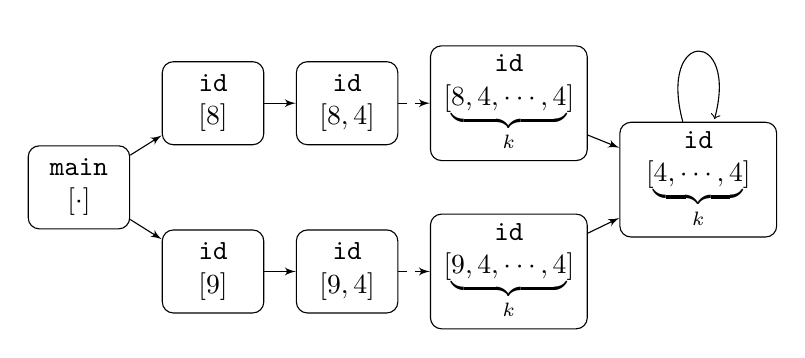
\begin{tikzpicture}
    \node [block] (main) {{\tt main} \\ $[\cdot]$};
    \node [block, above right=0cm and 0.4cm of main] (id1) {{\tt id}\\$[8]$};
    \node [block, below right=0cm and 0.4cm of main] (id2) {{\tt id}\\$[9]$};
    \node [block, right=0.4cm of id1] (id3) {{\tt id} \\$[8,4]$};
    \node [block, right=0.4cm of id2] (id4) {{\tt id} \\$[9,4]$};
    \node [block2, right=0.4cm of id3] (id5) {{\tt id}\\$[\underbrace{8,4,\cdots,4}_k]$};
    \node [block2, right=0.4cm of id4] (id6) {{\tt id}\\$[\underbrace{9,4,\cdots,4}_k]$};
    \node [block2, below right=-0.5cm and 0.4cm of id5] (id7) {{\tt id} \\$[\underbrace{4,\cdots,4}_{k}]$};

    \path [line] (main) -- (id1);
    \path [line] (main) -- (id2);
    \path [line] (id1) -- (id3);
    \path [line] (id2) -- (id4);
    \path [line, dashed] (id3) -- (id5);
    \path [line, dashed] (id4) -- (id6);
    \path [line] (id5) -- (id7);
    \path [line] (id6) -- (id7);
    \path [line] (id7) edge[loop above] ();
\end{tikzpicture}
}
\end{center}


\caption{Call-graph by $k$-CFA}
\label{fig:overview:kCFA}
\vspace{2ex}

\begin{center}
\resizebox{0.45\columnwidth}{!}{
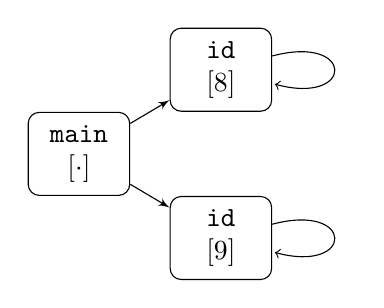
\begin{tikzpicture}
    \node [block] (main) {{\tt main}\\$[\cdot]$};
    \node [block, above right=0cm and 0.5cm of main] (id1) {{\tt id}\\$[8]$};
    \node [block, below right=0cm and 0.5cm of main] (id2) {{\tt id}\\ $[9]$};

    \path [line] (main) -- (id1);
    \path [line] (main) -- (id2);

    \path [line] (id1) edge[loop right] ();
    \path [line] (id2) edge[loop right] ();
\end{tikzpicture}
}
\end{center}
\caption{Call-graph by 1-CFA with tunneling}
\label{fig:overview:tunneling}
\end{subfigure}\qquad
\caption{Example and call-graphs constructed by the conventional
  $k$-call-site-sensitivity ($k$-CFA) and our 1-call-site-sensitivity
  with context tunneling}
\label{fig:overview}
\end{figure}




\myparagraph{Conventional Call-Site-Sensitivity}

The traditional $k$-call-site-sensitive analysis fails to prove the queries no matter what $k$ value is used.
Because the value of \texttt{i} can be any integer, the following set $K_{\infty}$ of infinite number of call-strings can be generated for method \texttt{id} at runtime:
\[
K_{\infty} = \myset{[8], [9], [8,4], [9,4], [8,4,4], [9,4,4], [8,4,4,4], [9,4,4,4], \dots}
\]
where, for example, $[8,4]$ denotes the context that method \texttt{id} was called along the sequence of
call-sites 8 and 4.
 The $k$-call-site-sensitive analysis approximates the call-strings in $K_{\infty}$ by their suffixes of length up to $k$. For example, when $k=2$, the analysis uses the following set $K_2$ of abstract contexts:
\[
K_2 = \myset{[8], [9], [8,4], [9,4], [4,4]}
\]
where an infinite number of contexts, $\myset{[8,4,4], [9,4,4], [8,4,4,4], [9,4,4,4],\dots}$, in $K_{\infty}$ are approximated by their common suffix $[4,4]$. The analysis analyzes the method \texttt{id} separately for each context in $K_2$. % producing the call-graph in Fig.~\ref{fig:overview}(b).
Although this approximation ensures termination, the analysis is now unable to differentiate the two separate calls to \texttt{id} at lines 8 and 9, causing the argument {\tt v} of {\tt id} to point to both objects {\tt A} and {\tt B} at the same time when the context becomes $[4,4]$. Thus, both objects get returned to both queries simultaneously, making the analysis fail to prove their cast safety.
Note that the analysis fails to prove the queries for any $k$ values, because all the context strings longer than $k$ are eventually
merged into a single context $[\underbrace{4,\dots,4}_{k}]$ (see
Fig.~\ref{fig:overview:kCFA}).


% the $k$-limited method is
% widely used in modern pointer
% analysis frameworks such as Doop~\cite{Bravenboer2009}.\minseok{redundant??}


% \minseok{
% 	Be aware that other kinds of context sensitivity like value context
% 	can prove the queries but	our goal is to overcome limitation of k-limiting context-sensitivity
% 	which is widely used.}
	
\myparagraph{Context Tunneling}

With context tunneling, however, even $1$-call-site sensitive analysis
becomes to prove the queries.
% Our idea to improve the analysis is to identify and maintain important
% context elements only.
The main weakness of the conventional
$k$-context-sensitive analysis is that it blindly updates the context
of a method at every call-site, thereby allowing important context
elements for the method to be easily overwritten by less important
ones.  In the example, distinguishing the two call-sites
at lines 8 and 9 is essential to proving the queries. However, this
information is eventually lost by repeatedly appending the less
important call-site 4 to the context of {\tt id}
(Fig.~\ref{fig:overview:kCFA}).
Our technique aims to overcome this weakness by maintaining important
context elements only during analysis. For example, we exclude the
call-site 4 from the context strings generated for method {\tt id} and
thus approximate the set $K_{\infty}$ to the set $K_T$ of contexts:
\[
K_T = \myset{[8], [9]}.
\]
Here abstract contexts $[8]$ and $[9]$ in $K_{T}$ denote the sets of concrete contexts
$\myset{[8], [8,4], [8,4,4], \dots}$ and
$\myset{[9], [9,4], [9,4,4], \dots}$ in $K_{\infty}$, respectively. The resulting
context-sensitive analysis with $K_{T}$ is able to prove the queries as it differentiates the two calls
to {\tt id} at lines 8 and 9 completely, producing the call-graph in
Fig.~\ref{fig:overview:tunneling}.

% With context tunneling, however, even $1$-call-site sensitive analysis
% is able to prove the queries.

\myparagraph{Challenge}

The example shows that the idea of context tunneling is potentially
powerful; even $1$-context-sensitivity with
tunneling can be as precise as
$\infty$-context-sensitivity. The goal of this chapter is to maximize
this tremendous, yet untapped, potential of the existing $k$-context-sensitive analysis.
However, achieving effective context tunneling in practice is
challenging. The effectiveness of the technique is very sensitive
to the choice of important context elements.  For example,
choosing the call-site 4, rather than call-sites 8 and 9, does not
work for the example program.  In the worst case, the analysis
precision degenerates into the context-insensitive case (e.g. when
selecting no context elements at all), becoming even inferior to the
ordinary
$k$-context-sensitive analysis.  Coming up with a good
heuristic rule for choosing important context elements is nontrivial;
hand-crafting such a rule not only requires a huge amount of
engineering effort and domain knowledge but also likely fails to
maximize the potential of the technique.
% adaptable as a fixed heuristic rule tuned for a particular situation
% may not be effective for other programs, analyses, or queries.


\myparagraph{Data-Driven Context Tunneling}


We address this challenge with a data-driven approach that
automatically learns a good heuristic rule for context tunneling from
a training set of programs.
Our aim is to generate a heuristic $\heuristic$,
% To do so, we first define a parameterized heuristic $\heuristic_\Pi$
% (where $\Pi$ is a parameter). $\heuristic_\Pi$
which takes a program and returns a relation $\TunnelingRelation$ on methods.
The relation contains a method pair $(m_1, m_2)$ if the calling context of
$m_1$ is more important than that of $m_2$. Thus, if $(m_1, m_2) \in
\TunnelingRelation$, the analysis applies context tunneling when $m_2$ is
invoked; that is, $m_2$ inherits the context of $m_1$ ignoring the current
context element. For the $k$-call-site-sensitivity example, $\heuristic_\Pi$
produces the relation $\TunnelingRelation = \myset{({\tt id}, {\tt id})}$,
which means that tunneling is applied when {\tt id} is called from {\tt id}.
As a result, the call-site 4, on which {\tt id} is called from {\tt id}, will
not be used as important context elements during analysis.  When {\tt main}
calls {\tt id}, however, the analysis updates the contexts as the ordinary
analysis since $({\tt main}, {\tt id}) \not\in \TunnelingRelation$.  In our
approach, the heuristic is parameterized and the parameter determines the
contents of the relation $\TunnelingRelation$.  The goal of our data-driven
technique is to characterize the two classes of methods: 1) methods that
increase the analysis precision by passing their contexts to others, and 2)
methods that increase the analysis precision by inheriting contexts from
others. Section~\ref{sec:learning} defines the learning problem and presents
an efficient algorithm to solve the problem.


%\subsection{Object-Sensitivity}
%
%The use of context tunneling is not limited to call-site-sensitivity.
%% Context tunneling is also effective for other flavors of
%% context-sensitivity.
%Below, we describe a typical situation where object-sensitivity
%benefits from context
%tunneling.
%
%%\lstset{
  language=Java,
  aboveskip=3mm,
  belowskip=3mm,
  showstringspaces=false,
  columns=flexible,
  basicstyle={\scriptsize\ttfamily},
  numbers=left,
  numbersep=5pt,
  numberstyle=\small\color{gray},
  keywordstyle=\color{blue},
  commentstyle=\color{dkgreen},
  stringstyle=\color{mauve},
  breaklines=true,
  breakatwhitespace=true,
  tabsize=3
}
\begin{figure}
\begin{subfigure}[b]{.9\columnwidth}
\begin{multicols}{2}
\centering
\begin{lstlisting}
class A {} class B {}
class C {
  public static void main (){
    ArrayList al1 = new ArrayList();//AL1
    ArrayList al2 = new ArrayList();//AL2

    al1.add(new A());
    al2.add(new B());

    Itr it1 = al1.iterator();
    Itr it2 = al2.iterator();

    A a = (A)it1.next();  //Query 1
    B b = (B)it2.next();  //Query 2
  }
}

class ArrayList{
  Object[] elementData = new Object[10];
  int size = 0;
  void add(Object e){
    elementData[size++] = e;
  }
  Itr iterator(){
    return new Itr(); //IT
  }
  class Itr{
    int cursor = 0;
    Object next(){
      return elementData[cursor++];
    }
  }
}
\end{lstlisting}
\end{multicols}
\caption{Example code}
\label{fig:obj:code}
\end{subfigure}
\begin{multicols}{2}
\begin{subfigure}[b]{.9\columnwidth}
\begin{center}
\resizebox{\columnwidth}{!}{
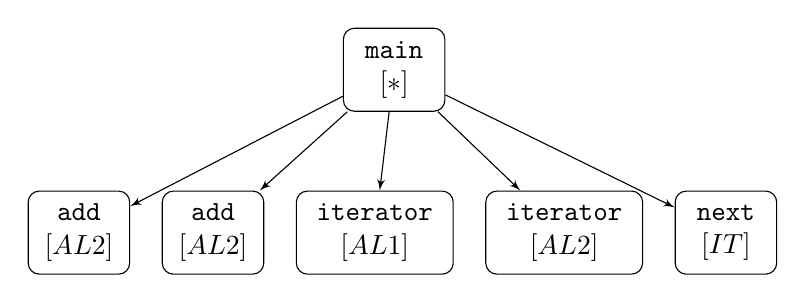
\begin{tikzpicture}
    \node [block] (main) {{\tt main}\\$[*]$};
    \node [block, below left=1cm and 2.7cm of main] (add1) {{\tt add}\\$[AL2]$};
    \node [block, right=0.4cm of add1] (add2) {{\tt add}\\$[AL2]$};
    \node [block2, right=0.4cm of add2] (iterator1) {{\tt iterator}\\ $[AL1]$};
    \node [block2, right=0.4cm of iterator1] (iterator2) {{\tt iterator}\\$[AL2]$};
    \node [block, right=0.4cm of iterator2] (next) {{\tt next}\\$[IT]$};

    \path [line] (main) -- (add1);
    \path [line] (main) -- (add2);
    \path [line] (main) -- (iterator1);
    \path [line] (main) -- (iterator2);
    \path [line] (main) -- (next);

\end{tikzpicture}
}
\end{center}
\caption{Call-graph by $1$-object-sensitive analysis}
\label{fig:obj:callgraph}
\end{subfigure}
\vfill\null
\columnbreak
\begin{subfigure}[b]{.9\columnwidth}
\begin{center}
\resizebox{\columnwidth}{!}{
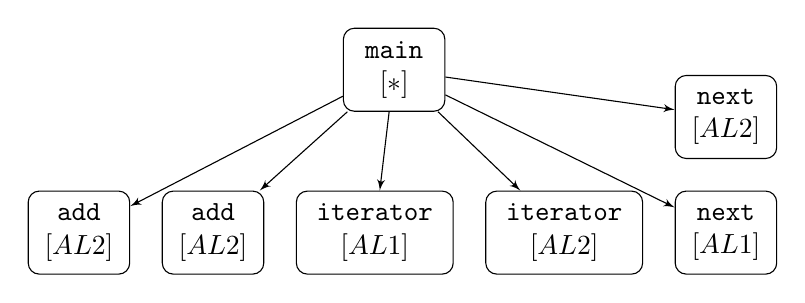
\begin{tikzpicture}
    \node [block] (main) {\tt main\\$[*]$};
    \node [block, below left=1cm and 2.7cm of main] (add1) {{\tt add}\\$[AL2]$};
    \node [block, right=0.4cm of add1] (add2) {\tt add\\$[AL2]$};
    \node [block2, right=0.4cm of add2] (iterator1) {\tt iterator\\$[AL1]$};
    \node [block2, right=0.4cm of iterator1] (iterator2) {\tt iterator\\$[AL2]$};
    \node [block, right=0.4cm of iterator2] (next1) {\tt next\\$[AL1]$};
    \node [block, above=0.4cm of next1] (next2) {\tt next\\$[AL2]$};

    \path [line] (main) -- (add1);
    \path [line] (main) -- (add2);
    \path [line] (main) -- (iterator1);
    \path [line] (main) -- (iterator2);
    \path [line] (main) -- (next1);
    \path [line] (main) -- (next2);

\end{tikzpicture}
}

\end{center}
\caption{Call-graph by $1$-object-sensitive analysis with tunneling}
\label{fig:obj:tunneling}
\end{subfigure}
\end{multicols}
\setlength{\abovecaptionskip}{-5pt}
\caption{Example code and callgraphs}
\label{fig:overviewObj}
\end{figure}

\myparagraph{Example Code for Object Sensitivity}
Example code in Fig.~\ref{fig:obj:code} present common pattern that 1-object-sensitive+heap
analysis lose precision. The main method use two data structure Arraylist, and it add
different data to each Arraylist. Main method makes iterator for each Arraylist and 
get data with iterators. The queries ask if two type casts at line 13 and 14 are
safe. 1-object-sensitive+heap analysis fails to prove the queries because
\texttt{next} method invoked in 13 and 14 are merged as
the method invocations have same context \texttt{IT}, 
constructing call-graph in Fig.~\ref{fig:obj:callgraph}. 

\myparagraph{Context Tunneling for Object sensitivity} 
With context tunneling, 1-object-sensitive+heap analysis can prove the queries. Note that Object sensitivity
has different flavor from call-site sensitivity; it updates context from heap context. Base
variable \texttt{it1} and \texttt{it2} point to same heap allocation but have different heap context: 
\texttt{AL1} and \texttt{AL2}. Applying context tunneling for \texttt{next} method make method call
at line 13 have context \texttt{AL1} and 14 have context \texttt{AL2},
resulting context sensitive analysis prove the queries with call-graph 
Fig.~\ref{fig:obj:tunneling}. 


%%% Local Variables:
%%% mode: latex
%%% TeX-master: "paper"
%%% End:

%\lstset{
%  language=Java,
%  aboveskip=3mm,
%  belowskip=3mm,
%  showstringspaces=false,
%  columns=flexible,
%  basicstyle={\scriptsize\ttfamily},
%  numbers=left,
%  numbersep=5pt,
%  numberstyle=\small\color{gray},
%  keywordstyle=\color{blue},
%  commentstyle=\color{dkgreen},
%  stringstyle=\color{mauve},
%  breaklines=true,
%  breakatwhitespace=true,
%  tabsize=3
%}
%\begin{figure}
%\begin{subfigure}[b]{0.9\columnwidth}
%\begin{multicols}{2}
%\centering
%\begin{lstlisting}
%class A {} class B {}
%class C {
%  public static void main (){
%    ArrayList al1 = new ArrayList();//AL1
%    ArrayList al2 = new ArrayList();//AL2
%
%    al1.add(new A());
%    al2.add(new B());
%
%    ArrayList.ListItr it1 = al1.iterator();
%    ArrayList.ListItr it2 = al2.iterator();
%
%    A a = (A)it1.next();  //Query 1
%    B b = (B)it2.next();  //Query 2
%  }
%}
%
%class ArrayList{
%  Object[] elementData = new Object[10];
%  int size = 0;
%  void add(Object e){
%    elementData[size++] = e;
%  }
%  ListItr iterator(){
%    return new ListItr(); //IT
%  }
%  class ListItr{
%    int cursor = 0;
%    Object next(){
%      return elementData[cursor++];
%    }
%  }
%}
%\end{lstlisting}
%\end{multicols}
%\caption{Example code}
%\label{fig:obj:code}
%\end{subfigure}
%\begin{multicols}{2}
%\begin{subfigure}[b]{.9\columnwidth}
%\begin{center}
%\resizebox{\columnwidth}{!}{
%\begin{tikzpicture}
%    \node [block] (main) {{\tt main}\\$[\cdot]$};
%    \node [block, below left=1cm and 2.7cm of main] (add1) {{\tt add}\\$[AL1]$};
%    \node [block, right=0.4cm of add1] (add2) {{\tt add}\\$[AL2]$};
%    \node [block2, right=0.4cm of add2] (iterator1) {{\tt iterator}\\ $[AL1]$};
%    \node [block2, right=0.4cm of iterator1] (iterator2) {{\tt iterator}\\$[AL2]$};
%    \node [block, right=0.4cm of iterator2] (next) {{\tt next}\\$[IT]$};
%
%    \path [line] (main) -- (add1);
%    \path [line] (main) -- (add2);
%    \path [line] (main) -- (iterator1);
%    \path [line] (main) -- (iterator2);
%    \path [line] (main) -- (next);
%
%\end{tikzpicture}
%}
%\end{center}
%\caption{Call-graph by $1$-object-sensitive analysis}
%\label{fig:obj:callgraph}
%\end{subfigure}
%\vfill\null
%\columnbreak
%\begin{subfigure}[b]{.9\columnwidth}
%\begin{center}
%\resizebox{\columnwidth}{!}{
%\begin{tikzpicture}
%    \node [block] (main) {\tt main\\$[\cdot]$};
%    \node [block, below left=1cm and 2.7cm of main] (add1) {{\tt add}\\$[AL1]$};
%    \node [block, right=0.4cm of add1] (add2) {\tt add\\$[AL2]$};
%    \node [block2, right=0.4cm of add2] (iterator1) {\tt iterator\\$[AL1]$};
%    \node [block2, right=0.4cm of iterator1] (iterator2) {\tt iterator\\$[AL2]$};
%    \node [block, right=0.4cm of iterator2] (next1) {\tt next\\$[AL1]$};
%    \node [block, above=0.4cm of next1] (next2) {\tt next\\$[AL2]$};
%
%    \path [line] (main) -- (add1);
%    \path [line] (main) -- (add2);
%    \path [line] (main) -- (iterator1);
%    \path [line] (main) -- (iterator2);
%    \path [line] (main) -- (next1);
%    \path [line] (main) -- (next2);
%
%\end{tikzpicture}
%}
%
%\end{center}
%\caption{Call-graph by $1$-object-sensitive analysis with tunneling}
%\label{fig:obj:tunneling}
%\end{subfigure}
%\end{multicols}
%\setlength{\abovecaptionskip}{-5pt}
%\caption{Example and call-graphs constructed by the conventional 1-object-sensitivity and our
%1-object-sensitivity with context tunneling}
%\label{fig:overviewObj}
%\end{figure}
%
%\myparagraph{Example Code}
%
%Fig.~\ref{fig:obj:code} shows
%a common code pattern that $1$-object-sensitivity with a context-sensitive heap
%loses precision, which is found frequently in data
%structure implementations such as List and Map.
%In the example code, we have four
%top-level classes, \texttt{A}, \texttt{B}, \texttt{C}, and
%\texttt{ArrayList}, and an inner class \texttt{ListIter} inside of the
%\texttt{ArrayList} class. The \texttt{ArrayList} class % , as the name suggests,
%% models on \texttt{java.util.ArrayList}, which is
%implements a resizable array.
%For simplicity, it maintains data in the % (fixed-size)
%\texttt{elementData} array and has the \texttt{add} method to append new data at
%the end of \texttt{elementData}. It also has the \texttt{iterator} method that
%returns an object of type \texttt{ListIter}, providing access to \texttt{elementData}.
%The \texttt{main} method in class \texttt{C} performs usual
%allocate-add-retrieve
%tasks using \texttt{ListIter}. The goal of the pointer
%analysis is to prove the safety of two type casts at lines 13
%and 14.
%
%\myparagraph{Conventional Object-Sensitivity}
%
%Conventional object-sensitivity analyzes different method calls
%separately for their base objects (and their heap contexts, if needed)~\cite{Smaragdakis2011}.  For
%example, when we analyze the \texttt{next} method at line 13,
%2-object-sensitivity creates the context $[\texttt{AL1},
%\texttt{IT}]$, where \texttt{IT} is the allocation-site of the base
%object (\texttt{it1}) and \texttt{AL1} is its heap context.
%Likewise, the
%method invocation at line 14 creates the context $[\texttt{AL2}, \texttt{IT}]$, enabling
%the analysis to distinguish the first and second calls to the same method. Using base objects
%as contexts makes object-sensitivity more favorable than
%call-site-sensitivity for object-oriented languages. However, it still
%updates contexts unconditionally at every method call and may lose important
%context elements when $k$ is not sufficiently large. For example, when we
%analyze the code with 1-object-sensitivity, the two calls to
%\texttt{next} are analyzed under the same context $[\texttt{IT}]$
%(Fig.~\ref{fig:obj:callgraph}).
%As a result, both objects \texttt{A} and \texttt{B} get returned to both
%queries simultaneously, making the analysis fail to prove the safety of type
%casting.
%
%
%
%\myparagraph{Object-Sensitivity with Context Tunneling}
%With context tunneling, however, even 1-object-sensitivity can prove the queries. Note that
%object-sensitivity has a different flavor from call-site-sensitivity; it
%updates the context with the heap context of the base object~\cite{Milanova2005, Milanova2002}. Base
%variables \texttt{it1} and \texttt{it2} point to the same heap allocation with different heap contexts: \texttt{AL1} and \texttt{AL2}. Applying context
%tunneling for the two method calls to \texttt{next} corresponds to
%propagating the heap contexts \texttt{AL1} and \texttt{AL2} at lines
%13 and 14, respectively, without modification.
%% makes the method call at line 13 to have
%% the context \texttt{AL1} and the method call at 14 to have the context \texttt{AL2}.
%The resulting context-sensitive analysis proves the queries with a call-graph
%shown in Fig.~\ref{fig:obj:tunneling}.


%%% Local Variables:
%%% mode: latex
%%% TeX-master: "paper"
%%% End:

%
\section{Overview}
\label{sec:overview}
This section exemplifies how our context tunneling approach.
\subsection{Context tunneling}
Suppose that we analyze the example Java code in Fig.~\ref{fig:overview:code} using flow-insensitive and context-sensitive points-to analysis. In this example code, we make calling contexts using call-site information. The example code has three classes, \texttt{A}, \texttt{B}, and \texttt{C}, and class \texttt{C} has two methods. Method \texttt{C.id(v, i)} is an identity function which returns an object passed to a formal parameter \texttt{v} after calling itself \texttt{i} times recursively. Method \texttt{C.main} calls \texttt{C.id} twice. Both invocation share same parameter \texttt{i} which is decided by user input but the first arguments are different. Finally, we want to prove safeness of two down casting operations at line 8 and 9 at run-time.

\begin{figure}
\centering
\begin{subfigure}[b]{.45\columnwidth}
\begin{lstlisting}
class A {} class B {}
class C {
  static Object id (Object v, int i){
      return i >= 0 ? id(v, i-1) : v;
  }
  public static void main (){
    int i = input();
    A a = (A) id(new A(), i);	//Q1
    B b = (B) id(new B(), i);	//Q2
  }
}
\end{lstlisting}
\caption{Example code}
\label{fig:overview:code}
\end{subfigure}\quad
\begin{subfigure}[b]{.45\columnwidth}
\begin{center}
\resizebox{\columnwidth}{!}{
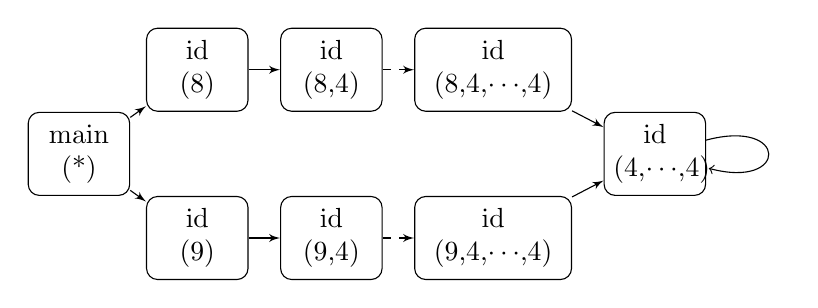
\begin{tikzpicture}
    \node [block] (main) {main\\(*)};
    \node [block, above right=0cm and 0.2cm of main] (id1) {id\\(8)};
    \node [block, below right=0cm and 0.2cm of main] (id2) {id\\(9)};
    \node [block, right=0.4cm of id1] (id3) {id\\(8,4)};
    \node [block, right=0.4cm of id2] (id4) {id\\(9,4)};
    \node [block2, right=0.4cm of id3] (id5) {id\\(8,4,$\cdots$,4)};
    \node [block2, right=0.4cm of id4] (id6) {id\\(9,4,$\cdots$,4)};
    \node [block, below right=0cm and 0.4cm of id5] (id7) {id\\(4,$\cdots$,4)};

    \path [line] (main) -- (id1);
    \path [line] (main) -- (id2);
    \path [line] (id1) -- (id3);
    \path [line] (id2) -- (id4);
    \path [line, dashed] (id3) -- (id5);
    \path [line, dashed] (id4) -- (id6);
    \path [line] (id5) -- (id7);
    \path [line] (id6) -- (id7);
    \path [line] (id7) edge[loop right] ();
\end{tikzpicture}
}
\end{center}
\caption{$k$-CFA callgraph}

\vspace{2ex}

\begin{center}
\resizebox{0.5\columnwidth}{!}{
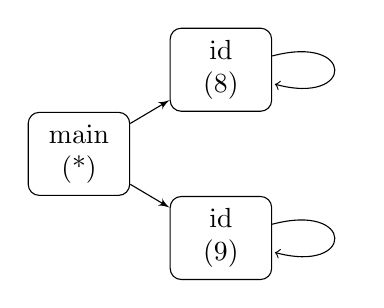
\begin{tikzpicture}
    \node [block] (main) {main\\(*)};
    \node [block, above right=0cm and 0.5cm of main] (id1) {id\\(8)};
    \node [block, below right=0cm and 0.5cm of main] (id2) {id\\(9)};

    \path [line] (main) -- (id1);
    \path [line] (main) -- (id2);

    \path [line] (id1) edge[loop right] ();
    \path [line] (id2) edge[loop right] ();
\end{tikzpicture}
}
\end{center}
\caption{1-callsite+T callgraph}
\end{subfigure}\qquad
\caption{Example code and callgraphs}
\label{fig:overview}
\end{figure}

Conventional $k$-callsite analysis with an arbitrary $k$ fails to prove all the queries. Because a sound static analyzer assumes an external user input \texttt{i} to be unbounded, no matter how large $k$ is chosen, $k^{th}$ and beyond invocations of method \texttt{C.id} are eventually merged and therefore formal argument \texttt{v} of method \texttt{C.id} points to objects of classes \texttt{A} and \texttt{B}. In other words, early context information (i.e., 8 and 9) that separates two call chains is wiped out by fresh but redundant context information (i.e., 4). As a result, the analysis concludes the method \texttt{C.id} can return an object of class \texttt{A} and \texttt{B}, which in turn causes invalid down casting alarm at line 8 and 9. Theoretically, $\infty$-callsite analysis can prove all the queries but it is obviously infeasible.

Our approach equips a heuristic that compares parent and child contexts and tells which one is more promising for the called method. Conventional analysis can be thought as one who blindly prefers child context over parent one. By using our heuristic, we can prove all the queries with only 1-callsite analysis. Suppose we have following relations.
\[
\TunnelingRelation({\texttt {C.id}}, {\texttt {C.id}})
\]
This relation means two things:
\begin{itemize}
  \item The first argument method provides context information to the second argument method. Since \texttt{C.id} is calls itself recursively, this relation is true for the example in this regard.
  \item The context made from the first argument is more important than a context made from the second argument. First invocation of \texttt{C.id} makes more important context than one who is called recursively in it, and this is true for the following recursions.
\end{itemize}

As a whole, we can translate the above relation into; \emph{``C.id invocations inside C.id shouldn't make a new calling context.''} Instead of making new calling context, method invocations that satisfies the relation inherit contexts from parent contexts. For example, \texttt{C.id} invocations inside \texttt{C.main} can make new contexts using their callsites, like conventional analysis. In contrary, the recursively called \texttt{C.id} invocations inherit their contexts from old contexts. By doing so, performing 1-callsite analysis is enough for the example code to carry two key context information, which are 8 and 9, over call chains and make analysis to prove all queries.

\subsection{Context tunneling approach overview}
Our approach takes three inputs: a parametric static analyzer, training programs and a set of atomic features that describe Java methods. The parametric analyzer equips a heuristic that tells which method invocation should inherit its calling contexts from parent context (i.e., in case of $k$-CFA, it is a caller's context) instead of its child context. We model the heuristic's behavior using boolean formulas. Training programs are just a set of Java programs without any predefined labels. Lastly, a set of atomic features describes syntactic or semantic properties of methods, such as method's return type or whether it belongs to a inner class or not. Suppose we have three atomic features over method definitions as follows;
\[
\afeatures=\myset{a_1, a_2, a_3}
\]
and assume two method definitions in Fig.~\ref{fig:overview:code} have the features as follows:
\begin{align}
  C.main=\myset{a_3}, \quad C.id=\myset{a_1, a_2}
\end{align}
Given three components, suppose our learning algorithm results two boolean formulas $f_prime$ and $f_second$, e.g.,
\[
f_1=a_1 \wedge \neg a_3, \\quad f_2=a_2\wedge \neg a_3 
\]
The first formula $f_1$ means \emph{very important methods} who are believed to make useful context information






Note that, our heuristic doesn't evaluate invocation's contexts as they are; instead, it abstracts methods from the contexts and then extracts feature vectors using the atomic features. For instance, suppose call-site sensitive analysis with depth 1 distinguished three method invocations in Fig.~\ref{fig:overview:code} using call-site labels (e.g., line numbers) as follows:
\begin{align}\label{eq:overview:invos}
C.id(8),\quad C.id(9),\quad C.id(4)
\end{align}
Our heuristic has a function \methof~to extract method from each context information. Applying the function over context information in \ref{eq:overview:invos} results a set of methods as follows:
\begin{align}\label{eq:overview:mths}
\methof(8)=C.id, \quad \methof(9)=C.id, \quad \methof(4)=C.id
\end{align}
Now suppose we have three atomic features over method definitions as follows:
\[
\afeatures=\myset{a_1, a_2, a_3}
\]
And suppose two methods in \ref{eq:overview:mths} have the features as follows:
\begin{align}
  C.main=\myset{a_3}, \quad C.id=\myset{a_1, a_2}
\end{align}
Given three input components, our learning algorithm outputs two boolean formulas $f_1$ and $f_2$ over the atomic features as follows:
\[
f_1=a_2\wedge \neg a_3, \qquad f_2=a_1 \wedge \neg a_3
\]
Two boolean formulas $f_1$ and $f_2$ mean \emph{important} and \emph{very important} methods respectively. A method in $f_1$ or $f_2$ makes possibly useful context information but our heuristic outweighes $f_2$ over $f_1$. That m

If a method invocation's child context satisfies $f_2$, our heuristic marks a method invocation as \emph{important per se} and let it to use the child context. For the unmarked method invocations, otherwise, the heuristic makes them to use parent contexts instead. The heuristic also prefers a parent context over child one if a invocation's child context is \emph{important per se} but its parent context satisfies $f_1$, which means \emph{very important}. 

\subsection{Learning context tunneling heuristics}
asdf 
%%% Local Variables:
%%% mode: latex
%%% TeX-master: "paper"
%%% End:
%\section{Context sensitive Context Tunneling}
\begin{comment}
\begin{figure}
\begin{multicols}{2}
\begin{lstlisting}
0:   Class A{} Class B{}
1:   Object id1(Object v, int i){
2:     return v;
3:   }
4:   Object id2(Object v, int i){
5:     return id1(v);
6:   }
7:  void main(){
8:    A a1 = (A)id1(new A());//Q1
9:    B b1 = (B)id1(new B());//Q2
10:   A a1 = (A)id2(new A());//Q1
11:   B b1 = (B)id2(new B());//Q2
12:   return;}
\end{lstlisting}
(a) Example Code\\
\begin{center}


\includegraphics[width=6cm,height=6cm,keepaspectratio]{figures/ctxTunnel.pdf}\\
(c) Context-sensitive tunneling
\end{center}
\end{multicols}
\caption{Tunneling considering context}
\label{fig:ExampleCode}
\end{figure} 
\end{comment}
\chapter{Data-driven Context Tunneling}\label{sec:Tunneling}
  In this chapter, we present our novel technique context tunneling and our data-driven approach for learning context tunneling heuristics.
  As context-sensitivity holds the key to the development
  of precise and scalable pointer analysis, a variety of techniques
  for context-sensitivity have been proposed. However, existing
  approaches such as $k$-call-site-sensitivity or $k$-object-sensitivity have a
  significant weakness that they unconditionally update the context of a
  method at every call-site, allowing important context elements to be
  overwritten by more recent, but not necessarily more important,
  context elements. In this chapter, we show that this is a key limiting factor of
  existing context-sensitive analyses, and demonstrate that remarkable increase in
  both precision and scalability can be gained by
  maintaining important context elements only.
  Our approach, called context tunneling, updates contexts selectively
  and decides when to propagate the same context without
  modification.



  We attain context tunneling via a data-driven approach.  The
  effectiveness of context tunneling is very sensitive to the choice
  of important context elements. Even worse, precision is not
  monotonically increasing with respect to the ordering of the
  choices. As a result, manually coming up with a good heuristic rule
  for context tunneling is extremely challenging and likely fails to
  maximize its potential. We address this challenge by developing a
  specialized data-driven algorithm, which is able to automatically
  search for high-quality heuristics over the non-monotonic space of
  context tunneling.

  We implemented our approach in the Doop framework and applied it to
  four major flavors of context-sensitivity: call-site-sensitivity,
  object-sensitivity, type-sensitivity, and hybrid context-sensitivity. In
  all cases, $1$-context-sensitive analysis with context
  tunneling far outperformed deeper context-sensitivity with $k=2$ in
  both precision and scalability.


\definecolor{dkgreen}{rgb}{0,0.6,0}
\definecolor{gray}{rgb}{0.5,0.5,0.5}
\definecolor{mauve}{rgb}{0.58,0,0.82}

\lstset{,language=Java, aboveskip=3mm, belowskip=3mm,
	showstringspaces=false, columns=flexible,
	basicstyle=\linespread{1.2}\small\ttfamily, numbers=left, numbersep=5pt,
	numberstyle=\small\color{gray}, keywordstyle=\color{blue},
	commentstyle=\color{dkgreen}, stringstyle=\color{mauve},
	breaklines=true, breakatwhitespace=true, tabsize=3 
}



% \tikzstyle{block} = [rectangle, draw, fill=white, text width=5em,
% text centered, rounded corners, minimum height=4em]

\tikzstyle{block} = [rectangle, draw, fill=white, text width=2.8em,
, text
centered, rounded corners, minimum height=3em]

%\tikzstyle{block2} = [rectangle,   text width=2em, text
%centered, rounded corners, minimum height=3em]

\tikzstyle{block2} =
[rectangle, draw, fill=white, text width=5em, text centered, rounded
corners, minimum height=4em, minimum width = 6em] \tikzstyle{line} = [draw, -latex']
\tikzstyle{onlyText} = [text width =2em, text centered]




\tikzstyle{myCircle} = [circle,thick,draw=black!75   text width=3.5em, text
centered, minimum height=3em]



\tikzstyle{line} = [draw, -latex']
\tikzstyle{onlyText} = [text width =5em, text centered]
\tikzstyle{smallOnlyText} = [text width =15em, text centered]
\tikzstyle{None} = [text width =0em, text centered]
\tikzstyle{longText} = [text width = 20em, text centered]

%\setcopyright{rightsretained}


\tikzstyle{block4} =
[rectangle, draw, fill=white, text width=9.5em, text centered, rounded
corners, minimum height=2.3em]
\tikzstyle{block3} =
[rectangle, draw, fill=white, text width=8em, text centered, rounded
corners, minimum height=2.3em] \tikzstyle{line} = [draw, -latex']


\tikzstyle{blocks} = [rectangle, draw, fill=white, text width=0.7cm, text
centered,  text width=4em, rounded corners, minimum height=0.5cm]











\section{Introduction}

\iffalse
Points-to analysis is a fundamental program analysis technique with
diverse applications in software engineering tasks.  The goal of
points-to analysis is to safely yet accurately approximate the objects
that pointer variables may point to at runtime, as precise pointer
information is a key ingredient of modern software analysis techniques
such as static bug-finding~\cite{Blackshear2015,Sui2014,Naik2006,Livshits2003,Avots2005},
program verification~\cite{Fink2008}, security vulnerability
detection~\cite{Tripp2009,Arzt2014,Yan2017}, and automatic program
repair~\cite{Gao2015,memfix}.  The effectiveness and
usefulness of these techniques are ultimately determined by the
qualities of the underlying points-to analysis.


Context-sensitivity holds the key to the development of precise and
scalable points-to analysis.  In order to accurately track local
variables and heap objects, a context-sensitive analysis treats
multiple calls to the same method separately for its different calling
contexts.  For object-oriented and functional languages,
context-sensitivity is the single most important factor that affects
both precision and scalability.  It has greater impact on the analysis
precision than other techniques such as
flow-sensitivity~\cite{Lhotak2006,Smaragdakis2015}, and the improved
precision by context-sensitivity is likely to increase scalability as
well~\cite{Smaragdakis2011, Kashyap2014}.
\fi


Developing effective approaches to context-sensitivity
has been the major goal of research in points-to analysis.  In
particular, 
one practical approach to context-sensitivity is the
so-called $k$-limited method~\cite{Sharir1981} and over the last
decades researchers have explored various flavors and policies with different
tradeoffs, such as object-sensitivity~\cite{Milanova2005},
type-sensitivity~\cite{Smaragdakis2011}, hybrid
context-sensitivity~\cite{KastrinisS13a}, and selective
context-sensitivity~\cite{JeJeChOh17,Oh2014,Smaragdakis2014}.  These approaches vary
depending on the program entities that they use as context elements or
policies to assign $k$ values. 
Unlike the classical $k$-call-site-sensitivity~\cite{Shivers1988},
object- and type-sensitivity use a sequence of allocation-sites and a
sequence of allocating-classes as context elements, respectively,
providing new sweet spots for object-oriented languages. Hybrid
context-sensitivity provides a way of combining call-site-sensitivity
and object-sensitivity to enjoy benefits of both approaches. Selective
context-sensitive analyses assign different $k$ values to different
methods. 


% \sehun{Another
% noteworthy approach is making call-string-based context-sensitivity more
% efficient without compromising precision by exploiting finite domains of
% method-reaching values~\cite{Khedker2008, PadhyeK13}.} In
% Section~\ref{sec:related}, we provide a more extensive survey on existing
% techniques.
% \minseok{Among two general ways to achieve context-sensitivity,
% \emph{functional} and \emph{call-strings} approaches~\cite{Sharir1981},
% approximated-version of call-string approach so called $k$-limiting
% context-sensitivity is widely used in practice.  As it is impractical to
% treat all the multiple calls to the same method separately, $k$-limiting
% context-sensitivity uses $k$ most recent context elements and merges method
% calls which have same context. In $k$-limiting context-sensitivity, it is
% important to choose suitable context element and depth $k$ because it decides
% precision and scalability of analysis.}

% \minseok{In this paper, we present context tunneling, a new approach for
% 	performing precise and scalable points-to
% 	analysis with k-limiting context-sensitivity.}


To develop an effective context abstraction, we present context tunneling, a new approach for
performing precise and scalable $k$-limited context-sensitive 
analysis. The key observation behind our approach is that, although
existing approaches for context-sensitivity differ in various
characteristics such as
flavors~\cite{Shivers1988,Milanova2005,Smaragdakis2011,KastrinisS13a}
and policies to assign $k$ values~\cite{Smaragdakis2014,JeJeChOh17,Oh2014},
they all have a significant weakness in common: they update the
context of a method unconditionally at {\em every} call-site and therefore important
context elements are overwritten by more recent, but not necessarily
more important, context elements. We found that this is a key factor
that limits the effectiveness of the existing context-sensitive
analyses, and show that dramatic increase in both precision and
scalability can be gained by maintaining important context elements
only. Our technique updates contexts selectively and decides when to
preserve contexts without modification. 
% \minseok{More specifically, we maintain \emph{caller}-\emph{callee} relations
% to represent situations that updating context at callee would lose key
% context elements. In such cases, the callee just inherits the key context
% from parent context, which is defined differently by context flavors, without
% modification.} 
We formalize our technique in a general setting, so that it is
applicable to all major flavors of context-sensitivity.


We also present a new data-driven approach for realizing effective context
tunneling.  Although the potential of context tunneling is
tremendous, maximizing its impact  in practice is nontrivial.  This is mainly
because precision increase by context tunneling is very sensitive to the
choice of important context elements and even not monotone with respect to the ordering of the
choices. As a result, manually coming up with a good heuristic rule
for context tunneling is extremely challenging and likely ends up with
suboptimal results.  To address this challenge, we leverage the recent
trend of data-driven program analysis~\cite{JeJeChOh17,Oh2015,
  Heo2016learning,heo2016unsound,WeiR15,Singh2018cav,ChOhHeYa17} and aim at automatically
learning a context-tunneling heuristic from data.  Given a dataset of
programs and a set of method features, our learning algorithm
generates a heuristic that determines the context elements that
contribute to improving the final analysis performance. Our algorithm
is carefully designed for context tunneling, so it is able to produce
effective heuristics over the non-monotonic space of context
tunneling.

% However, as the analysis with context tunneling
% is not monotone with respect to the analysis precision
% (Section~\ref{sec:setting}), finding a good tunneling heuristic is
% challenging. In particular, we cannot use the existing learning
% algorithms~\cite{JeJeChOh17,Liang2011learning} that work in a
% greedy manner by exploiting the monotonicity of the analysis.  We
% carefully designed a learning algorithm that interleaves a greedy
% refinement procedure with explorations and therefore is able to find a
% good parameter over the non-monotonic space of context tunneling (Section~\ref{sec:learning-algorithm}).



We implemented our approach on top of
the Doop framework~\cite{Bravenboer2009} and evaluated it with four
major flavors of context-sensitivity: call-site-sensitivity~\cite{Shivers1988},
object-sensitivity~\cite{Milanova2002, Milanova2005}, type-sensitivity~\cite{Smaragdakis2011},
and hybrid context-sensitivity~\cite{KastrinisS13a}.
In all analyses, context tunneling has improved the performance of the
existing analyses remarkably.
In particular, context tunneling enabled 1-context-sensitive analyses
to far outperform 2-context-sensitive
counterparts in both scalability and precision.
We also demonstrate that the effectiveness of context tunneling comes from our learning algorithm; we
evaluate our learning algorithm from various perspectives and justify
the design decisions underlying the algorithm.
% demonstrate that our non-greedy algorithm that deliberately performs
% explorations plays a central role for learning good tunneling
% heuristics.

\myparagraph{Contributions}
The contribution of this chapter is as follows:
\begin{itemize}
\item We present context tunneling, a new technique for
  improving $k$-limited context-sensitive points-to analysis by carefully maintaining
  important context elements. % context sensitive points-to analysis, and data-driven approach to
  % learn effective context tunneling heuristics in Boolean formulas
  % from codebase.

  \item We present a new data-driven approach for learning context
    tunneling heuristics. Key technical contribution is the non-greedy
    learning algorithm that is able to effectively search for good
    heuristics over non-monotonic parameter space of context
    tunneling.

  \item We extensively evaluate the effectiveness of context tunneling and our
    learning approach with for four flavors of context sensitive
    analysis for Java. % ; call-site, object, type, and hybrid context sensitivities. We also demonstrated that interleaving greedy search with exploration steps is key to success; fully-greedy variant of our algorithm converged toward less precise solutions early.
\end{itemize}



%  although keeping the most recent context
% elements is not always the most value choice. In fact, we found that
% blindly choosing the last $k$ context elements is a major factor may
% sacrifice the analysis scalability without increasing precision.  From
% the perspective of a call-site sensitivity, a place where a recursive
% method is invoked by others is far more significant than the place
% where the method calls itself.  To address this issue, our technique
% enables the analysis to maintain important contexts only. For example,
% method $m_1$ is called from method $m_2$ during 1-call-site-sensitive
% analysis, our analysis updates the context only when the new context
% is more important than the context of $m_2$. By doing so, with our
% technique, a sequence of context elements contains only valuable
% context elements which contribute to increase analysis precision.


% abstract a program's possibly infinite concrete contexts into
% computable one is to limit the maximum length of calling
% contexts. And the most dominant way to do it is concatenating the
% most recent $k$ context elements. For example, in
% $k$-call-site-sensitivity~\cite{Shivers1988,Sharir1981}, the
% analysis maintains a sequence of the last $k$ call-sites that lead
% to each method call. Although the existing context-sensitive
% points-to analyses differ in various characteristics (e.g. which
% context elements to
% use~\cite{Milanova2005,Smaragdakis2011,kastrinis2013hybrid}, which
% $k$ values to assign to different
% call-sites~\cite{Smaragdakis2014,JeJeChOh17}, etc), this recency
% property remains in common.

% However, the most recent context element may not the most valuable one.
% Recursion is the prime example. From the perspective of a call-site sensitivity,
% a place where a recursive method is invoked by others is far more significant
% than the place where the method calls itself. Same story goes for an object
% sensitivity, which uses heap allocation sites as context elements, too. Some classes have limited allocation sites as they only exist to comprise higher-level classes. In this case, the ``helper'' classes' allocation sites are likely less significant than the ones of the composite classes although the helper objects are relatively new than the composite objects. Problem is, knowing such cases for a wide range
% of context abstractions and infusing the knowledge into static analyzers without negative side-effects is highly non-trivial.
%Current context sensitivity, however, wastes given depth $k$ by blindly generating context elements and updating methods' context whenever they are invoked. As each method use most-recent-$k$ context elements as its context, generating new context elements results losing old context elements that would play a key role for the method. As a result, many methods lose their key context elements by updating contexts resulting lose of both precision and scalability.

% In this paper, we present context tunneling, a general approach for improving
% scalability and precision of context-sensitive points-to analysis. Key idea is not
% updating methods's context but inheriting old contexts from parent methods when it is
% considered to be beneficial. Our heuristic expresses such situations in relations
% between two methods $(m_1, m_2)$. This relation states that if a method $m_2$ is invoked
% under a parent method $m_1$, the called method $m_2$ should inherit $m_1$'s context
% instead of making new context element. Recall the previous call-site example, context
% tunneling heuristic with $(\texttt{rec}, \texttt{rec})$ relation keeps recursively
% called $\texttt{rec}$ methods to generate redundant context elements. This
% representation introduces the unusual characteristic that most known parameters in
% designing static analyzer don't: precision doesn't monotonically increase (or decrease)
% as we apply context tunneling to more methods. In fact, as context tunneling is applied
% for more methods from nought, the analysis changes from conventional context sensitivity
% to context-insensitive one; the most desirable heuristic is somewhere in between. It
% falsifies the greedy approach, taking the largest benefit after evaluating small changes
% from current state, thus achieving the goal of context tunneling --- finding a set of
% method relations for target program that maximizes precision while not
% losing scalability --- becomes extremely difficult.

% %This simple mechanism can extend key contexts' lifespan
% %indefinitely thus contributes to realize potential of $k$-limited context
% %sensitive points-to analysis.
% We use data-driven approach to automatically learn tunneling heuristic from codebase.
% The learning algorithm is specifically designed around the problem of context tunneling
% as it choices apparently bad refinement to see if the decision results better outcome at
% the end. First, we parameterize context tunneling heuristic. We use disjunctive
% parameter model introduced in~\citet{JeJeChOh17} for expressiveness. That is, the
% heuristic's parameter is a set of two Boolean formulas $f_1$ and $f_2$ where
% $f_i$ is a Boolean combination of atomic features that captures high-level property of
% Java method for $m_i$. The atomic features are simple predicates over Java methods like
% whether method has heap allocations or not. A heuristic ($f_1,f_2$) means a set of
% context tunneling relations ($m_1$, $m_2$) where $f_i$ means a set of methods $m_i$.
% Than, we propose new learning algorithm to find the good parameters $f_1$ and $f_2$.
% Key technical idea is interleaving greedy refinement procedure with explorations. In the
% exploration steps, our algorithm opts for the most exclusively provable queries, not
% immediate precision gain. The choice is further refined in greedy fashion and approved if the refined one increases parameter's precision without cost explosion.
%
%
%
%Key technical challenge is finding the good parameters $f_1$ and $f_2$ efficiently as
%brute-force methods simply cannot cope with the large parameter space, and more
%importantly, we can't leverage prior learning algorithms are unable to learn desirable heuristic as this
%new parameter space is not equipped with precision order that previous learning
%algorithm~\cite{JeJeChOh17,Liang2011learning,Zhang2014} heavily
%relied on. In this paper, we designed new learning algorithm that searches the
%parameter space of context tunneling effectively. Key idea to overcoming
%challenges is evaluating intermediate formula's
%quality by counting exclusively proven queries rather than immediate precision gain. By doing so, our algorithm finds much more effective tunneling heuristics than learned one with seeing only immediate precision. Our learning algorithm also concerns cost aspect so the resulting parameters don't make analysis more costly than the conventions.


%More precisely, our approach provides a heuristic to a static analyzer that tells
%where to apply context tunneling technique for a given program. The heuristic express
%such places using a set of relations $(m_1, m_2)$ between two methods in target
%program. This relation states that if a method $m_2$ is invoked under a parent method
%$m_1$, the called method $m_2$ should inherit $m_1$'s context. In previous call-site
%example, $(rec, rec)$ means such case if we refer $rec$ to the recursive method.
%Key challenge is that good context tunneling heuristics that generally work
%well on target programs are difficult to find, and incompetent one can propagate
%worthless contexts indefinitely thus degrades precision as a level of
%context-insensitive analysis.
%
%To solve the search problem, we use data-driven approach, which is gaining popularity
%in fine-tuning static analyzers
%recently~\cite{JeJeChOh17,Oh2015,Heo2016learning,cha2016learning,WeiR15}.
%First, we design a set of atomic features; each one of them is a Boolean predicate
%over Java methods such as whether it has heap allocations or not. Than, we
%parameterize context tunneling heuristic using two Boolean formulas $f_1$ and $f_2$.
%Each Boolean formula is a Boolean combination of the atomic features and means a set
%of methods in target program where $f_i$ means methods take the place of $m_i$ in
%context tunneling relations. Finding a good set of parameters $f_1$ and $f_2$ that
%maximizes analysis precision of given while not losing scalability is done by a
%learning algorithm we specifically designed around the problem of context tunneling.


%to obtain such good context tunneling heuristics automatically from existing codebase. First, we design a set of atomic features; each one of them is a Boolean predicate over Java methods such as whether it has heap allocations or not. Than, we design a learning algorithm that infers two formulas $f_1$ and $f_2$ where $f_i$ is a Boolean combination of atomic features. The goal of learning algorithm is to find a good set of $f_1$ and $f_2$ so that two methods from each formula constitute a set of tunneling relation tuple $(m_1, m_2)$ correspondingly. That is, those two Boolean formula become a parameter of context tunneling heuristic.
%%In our approach, relations between two methods express situations that applying context tunneling has benefit. Each relation states that if a method is invoked under a parent method and the two methods are belong to the relation, called method should inherit context from parent method's context.
%The goal of learning process is to find a good set of tunneling parameters $f_1$ and $f_2$ that maximizes analysis precision of given while not losing scalability.
%
%We use data-driven approach to obtain desirable context tunneling abstraction automatically. In our approach, analyzer is equipped with a parameterized and heuristic rules that decide whether to apply context tunneling. Key technical challenge is finding the good parameters efficiently as brute-force methods simply cannot cope with the large parameter space. Unfortunately, previous data driven approaches~\cite{JeJeChOh17,Oh2015,Heo2016learning,cha2016learning} is unable to learn appropriate context tunneling heuristic because abstraction space in context tunneling is not equipped with precision order which is assumed in previous works. We designed new non-greedy learning algorithm that efficiently learn context tunneling heuristic. Key idea is evaluating intermediate formula's quality by measuring potential rather than immediate precision gain. Our learning algorithm also concerns cost aspect so the resulting parameters don't make analysis more costly than the conventions.

% The experimental results show generality and effectiveness of our approach; well-trained context tunneling heuristics make $1$-context sensitivity more precise and scalable than the deeper counterparts. We implemented our approach on Doop Java points-to analysis framework~\cite{Bravenboer2009} and applied to four well-known context sensitivities; call-site~\cite{Shivers1988,Sharir1981}, object~\cite{Milanova2002, Milanova2005}, type~\cite{Smaragdakis2011}, and hybrid context~\cite{kastrinis2013hybrid} sensitivities. For all analyses, $1$-context sensitive analyses with context tunneling are more precise than conventional analyses with deeper context $k=2$ without increasing cost. In fact, our approach is so effective for hybrid context sensitivity so that our version ($\onesobjHT$) was able to analyze all prepared benchmarks in time while less precise $\twosobjH$ violated the time constraint (5,400 sec) when analyzing \texttt{jython}.

% In summary, our key contributions are as follow:
% \begin{itemize}
%   \item We introduce context tunneling, a new parameter space for context sensitive points-to analysis, and data-driven approach to learn effective context tunneling heuristics in Boolean formulas from codebase.
%   \item We demonstrated effectiveness of context tunneling for four kinds of context sensitivities; call-site, object, type, and hybrid context sensitivities. We also demonstrated that interleaving greedy search with exploration steps is key to success; fully-greedy variant of our algorithm converged toward less precise solutions early.
% \end{itemize}



\commentout{
Conventional context-sensitive analysis generates and utilzes contexts without considering any. Contexts, however, should be carefully generated because generating a useless context often results pushing off key contexts.
\\
Fig.\ref{fig:ExampleCode}(a) is an Example to illustrate how conventional context sensitive analysis lose precision and how context-tunneling handles the problem. In Fig.\ref{fig:ExampleCode}, we identify 2 heap allocations(A, B), 3 method call-sites(3, 7, 10) and 2 queries(Q1, Q2) with end-of-line comments in green. Method id is recursively defined identity funtion that always returns first parameter v. Method assginA(assignB) allocate heap object typed A(B) call id with the object and input parameter i. main method calls assignA and assignB with input integer i and queries ask safety of down castings. In Fig.\ref{fig:ExampleCode}(b), we give call graph of conventional k-call-site sensitive analysis, where each method is analyzed separately for each different calling context.
\\
As can be seen in Fig.\ref{fig:ExampleCode}(b), context 14 and 15 are key contexts that separate id methods called from assignA and that from assignB. However, contexts generated from call-site 3 push off the key contexts whenever it is called. Methods id called from assignA and  methods called from assignB are eventually merged. As a result, variable a and b can point to A and B, respectively.
\\
To address the problem that useless context disturb analysis, we propose context-tunneling, a general approach for improving precision of context-sensitive analysis. Key idea is inheriting meaningful contexts from ancestor methods by recycling the meaningful contexts as decendant methods' contexts. Let assume we know call-site 14 and 15 are the only key contexts of Fig.\ref{fig:ExampleCode}(a) and the other contexts are worthless. Under the assumption, we give call-graph of 1-call-site sensitive+Tunnel in Fig.\ref{fig:ExampleCode}(c). Now, id methods called from assignA and that from assignB are analyzed separately. Due to the improvements of precision, a (b) now points to A (B) only, causing may-alias to conclude that both are no longer alias and resulting analyzer proves the safety of the queries. In conventional call-site-sensitive anlaysis, such precision can only be obtained from $\infty$-call-site-sensitive analysis.
%Context-tunneling is generally appliable approach that can be applied to any kinds of context,e.g., call-site sensitivity, object-sensitivity and type-sensitivity.
\\
Although context-tunneling has potential to increase precision significantly, it is another issue to judge usefulness of each context. We used data-driven approach to get a classifier for tunneling approach. In data-driven appraoch, We used disjunctive model to express heuristic and designed 25 features. We designed a new learning algorithm as context-tunneling has different properties from other previous instances, e.g., selective-context-sensitivity. From codebase, our learning algorithm automatically learns appropriate context-tunneling heuristics with disjunctive model and features. The experimental results show that learned heuristics improve precision significantly. For example, applying context-tunneling to 1-object-sensitive+heap shows nearly equal precision to conventional 3-object-sensitive+3-heap in Java Points-to analysis. In summary, our key contributions are as follows:
\begin{itemize}
\item{We propose "Context-Tunneling", a general approach for improving precision of context-sensitive analysis.}
\item{We designed a new learning algorithm to obtain effective tunnel from code base.}
\item{We demonstrate the effectiveness of our approach with applications to object sensitivity in Java Points-to analysis.}
\end{itemize}

\begin{figure}
\begin{multicols}{2}
\begin{lstlisting}
Class A{} Class B{}
Object id(Object v, int i) {
  if(i>=0){
   return id(i-1, v);}  //3
  else{return v;}
}
Object assignA(int i) {
 return id(new A(),i);  //A,7
};
Object assignB(int i) {
 return id(new B(),i);  //B,10
};
void main() {
  int i = input();
  A a = (A)assignA(i);  //Query 1
  B b = (B)assignB(i);  //Query 2
 return;
}
\end{lstlisting}
(a) Example Code\\
\begin{center}
\includegraphics[width=7cm,height=7cm,keepaspectratio]{figures/standard.pdf}\\
(b) Conventional k-call-site-sensitive
\includegraphics[width=6cm,height=6cm,keepaspectratio]{figures/important.pdf}\\
(c) 1-call-site-sensitive+tunnel
\end{center}
\end{multicols}
\caption{Motivating Example}
\label{fig:ExampleCode}
\end{figure}
}

% \begin{figure}
% \begin{multicols}{2}
% \begin{lstlisting}
% 0:   Class A{} Class B{}
% 1:   Object id(Object v, int i){
% 2:     if(i>=0){
% 3:      return id(i-1, v);}//3
% 4:     else{return v;}
% 5:   }
% 6:   Object assignA(int i){
% 7:    return id(new A(),i);//A,7
% 8:   };
% 9:   Object assignB(int i){
% 10:   return id(new B(),i);//B,10
% 11:  };
% 12:  void main(){
% 13:    int i = input();
% 14:    A a = (A)assignA(i);//Q1
% 15:    B b = (B)assignB(i);//Q2
% 16:   return;}
% \end{lstlisting}
% (a) Example Code\\
% \begin{center}

% \includegraphics[width=7cm,height=7cm,keepaspectratio]{figures/standard.pdf}\\
% (b) Conventional k-call-site-sensitive

% \includegraphics[width=6cm,height=6cm,keepaspectratio]{figures/important.pdf}\\
% (c) 1-call-site-sensitive+tunnel
% \end{center}
% \end{multicols}
% \caption{Theoretical Example}
% \label{fig:ExampleCode}
% \end{figure}


%%% Local Variables:
%%% mode: latex
%%% TeX-master: "paper"
%%% End:

%\newpage

\section{Motivating Examples}
\label{sec:overview}

In this section, we illustrate context tunneling with examples.
We describe our technique with $k$-call-site-sensitivity, but it is applicable to other flavors of
context-sensitivity too. The general description
is presented in Section~\ref{sec:tunneling}.

% \sehun{To
% show existence of aforementioned $k$-limiting context-sensitivity's
% limitation regardless of choice of context flavor, our examples are designed
% around two major principles, $k$-limiting call-site-sensitivity and
% $k$-object sensitivity. But it is also applicable to other flavors of
% context-sensitivity too, such as type-sensitivity.}

% \myparagraph{Caveat}
In this section, we restrict our discussion to the
traditional $k$-limited context-sensitive analysis. % Although the example
% programs in this section could be analyzed precisely with
Other approaches
such as value-based context-sensitivity~\cite{Khedker2008}
may not suffer from the issue described in this section.
However, their applicability to real-world pointer analysis remains to
be seen, which is beyond the scope of this chapter. On the other hand,
the $k$-limited method is more widely used in practical settings~\cite{Bravenboer2009,Smaragdakis2011,KastrinisS13a,Smaragdakis2014,JeJeChOh17}.



%applying them to real-world programs remains to be seen and is beyond the scope of this paper.
% On the other hand, the $k$-limited method is popular in practical settings~\cite{Bravenboer2009,Smaragdakis2011,kastrinis2013hybrid,Smaragdakis2014,JeJeChOh17}.


% The goal and scope of this paper are to identify and fix the
% major weakness of $k$-limited context-sensitive analysis that is
% widely used in modern pointer
% analyses~\cite{Bravenboer2009,Smaragdakis2011,kastrinis2013hybrid,Smaragdakis2014,JeJeChOh17}.
% Applying other methods such as value
% contexts~\cite{Khedker2008} to avoid the problem is beyond the scope of
% this paper.

\subsection{Call-Site-Sensitivity}
\myparagraph{Example Code}

Suppose that we analyze the example Java code in
Fig.~\ref{fig:overview:code} using a $k$-call-site-sensitive pointer
analysis~\cite{Smaragdakis2015}.  The example code has three class
definitions, namely \texttt{A}, \texttt{B}, and \texttt{C}.  Classes
\texttt{A} and \texttt{B} are empty and class \texttt{C} has two
methods: \texttt{id} and \texttt{main}.  Method \texttt{id} is
essentially the identity function on the first argument, which takes an
object \texttt{v} and an integer \texttt{i}, and returns the same
object after making recursive calls until \texttt{i} becomes 0. In
\texttt{main}, \texttt{id} is invoked twice with different
objects. Both method invocations share the same argument \texttt{i}
that comes from the external environment (i.e. user input).  The goal
of the pointer analysis is to prove the safety of two type casts at
lines 8 and 9.

\begin{figure}
\hspace*{0.1cm}
\centering
\begin{subfigure}[b]{.49\columnwidth}
\begin{lstlisting}
class A {} class B {}
class C {
  static Object id (Object v, int i){
    return i >= 0 ? id(v, i-1) : v;
 }
 public static void main (){
   int i = input();
   A a = (A) id(new A(), i);//Query 1
   B b = (B) id(new B(), i);//Query 2
 }
}
\end{lstlisting}
\caption{Example code}
\label{fig:overview:code}
\end{subfigure}
\quad
\hspace*{-1.cm}
\begin{subfigure}[b]{.45\columnwidth}

%%% k-CFA
\begin{center}
\resizebox{\columnwidth}{!}{
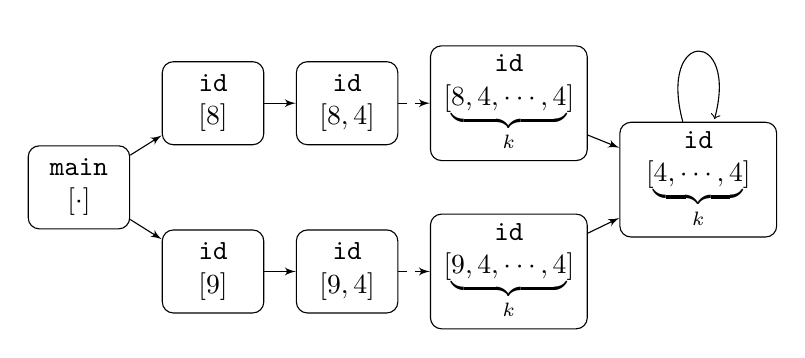
\begin{tikzpicture}
    \node [block] (main) {{\tt main} \\ $[\cdot]$};
    \node [block, above right=0cm and 0.4cm of main] (id1) {{\tt id}\\$[8]$};
    \node [block, below right=0cm and 0.4cm of main] (id2) {{\tt id}\\$[9]$};
    \node [block, right=0.4cm of id1] (id3) {{\tt id} \\$[8,4]$};
    \node [block, right=0.4cm of id2] (id4) {{\tt id} \\$[9,4]$};
    \node [block2, right=0.4cm of id3] (id5) {{\tt id}\\$[\underbrace{8,4,\cdots,4}_k]$};
    \node [block2, right=0.4cm of id4] (id6) {{\tt id}\\$[\underbrace{9,4,\cdots,4}_k]$};
    \node [block2, below right=-0.5cm and 0.4cm of id5] (id7) {{\tt id} \\$[\underbrace{4,\cdots,4}_{k}]$};

    \path [line] (main) -- (id1);
    \path [line] (main) -- (id2);
    \path [line] (id1) -- (id3);
    \path [line] (id2) -- (id4);
    \path [line, dashed] (id3) -- (id5);
    \path [line, dashed] (id4) -- (id6);
    \path [line] (id5) -- (id7);
    \path [line] (id6) -- (id7);
    \path [line] (id7) edge[loop above] ();
\end{tikzpicture}
}
\end{center}


\caption{Call-graph by $k$-CFA}
\label{fig:overview:kCFA}
\vspace{2ex}

\begin{center}
\resizebox{0.45\columnwidth}{!}{
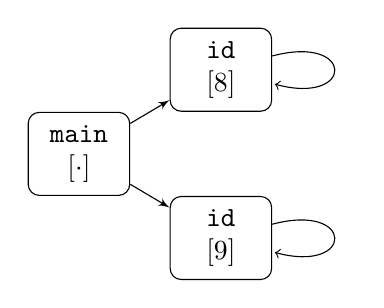
\begin{tikzpicture}
    \node [block] (main) {{\tt main}\\$[\cdot]$};
    \node [block, above right=0cm and 0.5cm of main] (id1) {{\tt id}\\$[8]$};
    \node [block, below right=0cm and 0.5cm of main] (id2) {{\tt id}\\ $[9]$};

    \path [line] (main) -- (id1);
    \path [line] (main) -- (id2);

    \path [line] (id1) edge[loop right] ();
    \path [line] (id2) edge[loop right] ();
\end{tikzpicture}
}
\end{center}
\caption{Call-graph by 1-CFA with tunneling}
\label{fig:overview:tunneling}
\end{subfigure}\qquad
\caption{Example and call-graphs constructed by the conventional
  $k$-call-site-sensitivity ($k$-CFA) and our 1-call-site-sensitivity
  with context tunneling}
\label{fig:overview}
\end{figure}




\myparagraph{Conventional Call-Site-Sensitivity}

The traditional $k$-call-site-sensitive analysis fails to prove the queries no matter what $k$ value is used.
Because the value of \texttt{i} can be any integer, the following set $K_{\infty}$ of infinite number of call-strings can be generated for method \texttt{id} at runtime:
\[
K_{\infty} = \myset{[8], [9], [8,4], [9,4], [8,4,4], [9,4,4], [8,4,4,4], [9,4,4,4], \dots}
\]
where, for example, $[8,4]$ denotes the context that method \texttt{id} was called along the sequence of
call-sites 8 and 4.
 The $k$-call-site-sensitive analysis approximates the call-strings in $K_{\infty}$ by their suffixes of length up to $k$. For example, when $k=2$, the analysis uses the following set $K_2$ of abstract contexts:
\[
K_2 = \myset{[8], [9], [8,4], [9,4], [4,4]}
\]
where an infinite number of contexts, $\myset{[8,4,4], [9,4,4], [8,4,4,4], [9,4,4,4],\dots}$, in $K_{\infty}$ are approximated by their common suffix $[4,4]$. The analysis analyzes the method \texttt{id} separately for each context in $K_2$. % producing the call-graph in Fig.~\ref{fig:overview}(b).
Although this approximation ensures termination, the analysis is now unable to differentiate the two separate calls to \texttt{id} at lines 8 and 9, causing the argument {\tt v} of {\tt id} to point to both objects {\tt A} and {\tt B} at the same time when the context becomes $[4,4]$. Thus, both objects get returned to both queries simultaneously, making the analysis fail to prove their cast safety.
Note that the analysis fails to prove the queries for any $k$ values, because all the context strings longer than $k$ are eventually
merged into a single context $[\underbrace{4,\dots,4}_{k}]$ (see
Fig.~\ref{fig:overview:kCFA}).


% the $k$-limited method is
% widely used in modern pointer
% analysis frameworks such as Doop~\cite{Bravenboer2009}.\minseok{redundant??}


% \minseok{
% 	Be aware that other kinds of context sensitivity like value context
% 	can prove the queries but	our goal is to overcome limitation of k-limiting context-sensitivity
% 	which is widely used.}
	
\myparagraph{Context Tunneling}

With context tunneling, however, even $1$-call-site sensitive analysis
becomes to prove the queries.
% Our idea to improve the analysis is to identify and maintain important
% context elements only.
The main weakness of the conventional
$k$-context-sensitive analysis is that it blindly updates the context
of a method at every call-site, thereby allowing important context
elements for the method to be easily overwritten by less important
ones.  In the example, distinguishing the two call-sites
at lines 8 and 9 is essential to proving the queries. However, this
information is eventually lost by repeatedly appending the less
important call-site 4 to the context of {\tt id}
(Fig.~\ref{fig:overview:kCFA}).
Our technique aims to overcome this weakness by maintaining important
context elements only during analysis. For example, we exclude the
call-site 4 from the context strings generated for method {\tt id} and
thus approximate the set $K_{\infty}$ to the set $K_T$ of contexts:
\[
K_T = \myset{[8], [9]}.
\]
Here abstract contexts $[8]$ and $[9]$ in $K_{T}$ denote the sets of concrete contexts
$\myset{[8], [8,4], [8,4,4], \dots}$ and
$\myset{[9], [9,4], [9,4,4], \dots}$ in $K_{\infty}$, respectively. The resulting
context-sensitive analysis with $K_{T}$ is able to prove the queries as it differentiates the two calls
to {\tt id} at lines 8 and 9 completely, producing the call-graph in
Fig.~\ref{fig:overview:tunneling}.

% With context tunneling, however, even $1$-call-site sensitive analysis
% is able to prove the queries.

\myparagraph{Challenge}

The example shows that the idea of context tunneling is potentially
powerful; even $1$-context-sensitivity with
tunneling can be as precise as
$\infty$-context-sensitivity. The goal of this chapter is to maximize
this tremendous, yet untapped, potential of the existing $k$-context-sensitive analysis.
However, achieving effective context tunneling in practice is
challenging. The effectiveness of the technique is very sensitive
to the choice of important context elements.  For example,
choosing the call-site 4, rather than call-sites 8 and 9, does not
work for the example program.  In the worst case, the analysis
precision degenerates into the context-insensitive case (e.g. when
selecting no context elements at all), becoming even inferior to the
ordinary
$k$-context-sensitive analysis.  Coming up with a good
heuristic rule for choosing important context elements is nontrivial;
hand-crafting such a rule not only requires a huge amount of
engineering effort and domain knowledge but also likely fails to
maximize the potential of the technique.
% adaptable as a fixed heuristic rule tuned for a particular situation
% may not be effective for other programs, analyses, or queries.


\myparagraph{Data-Driven Context Tunneling}


We address this challenge with a data-driven approach that
automatically learns a good heuristic rule for context tunneling from
a training set of programs.
Our aim is to generate a heuristic $\heuristic$,
% To do so, we first define a parameterized heuristic $\heuristic_\Pi$
% (where $\Pi$ is a parameter). $\heuristic_\Pi$
which takes a program and returns a relation $\TunnelingRelation$ on methods.
The relation contains a method pair $(m_1, m_2)$ if the calling context of
$m_1$ is more important than that of $m_2$. Thus, if $(m_1, m_2) \in
\TunnelingRelation$, the analysis applies context tunneling when $m_2$ is
invoked; that is, $m_2$ inherits the context of $m_1$ ignoring the current
context element. For the $k$-call-site-sensitivity example, $\heuristic_\Pi$
produces the relation $\TunnelingRelation = \myset{({\tt id}, {\tt id})}$,
which means that tunneling is applied when {\tt id} is called from {\tt id}.
As a result, the call-site 4, on which {\tt id} is called from {\tt id}, will
not be used as important context elements during analysis.  When {\tt main}
calls {\tt id}, however, the analysis updates the contexts as the ordinary
analysis since $({\tt main}, {\tt id}) \not\in \TunnelingRelation$.  In our
approach, the heuristic is parameterized and the parameter determines the
contents of the relation $\TunnelingRelation$.  The goal of our data-driven
technique is to characterize the two classes of methods: 1) methods that
increase the analysis precision by passing their contexts to others, and 2)
methods that increase the analysis precision by inheriting contexts from
others. Section~\ref{sec:learning} defines the learning problem and presents
an efficient algorithm to solve the problem.


%\subsection{Object-Sensitivity}
%
%The use of context tunneling is not limited to call-site-sensitivity.
%% Context tunneling is also effective for other flavors of
%% context-sensitivity.
%Below, we describe a typical situation where object-sensitivity
%benefits from context
%tunneling.
%
%%\lstset{
  language=Java,
  aboveskip=3mm,
  belowskip=3mm,
  showstringspaces=false,
  columns=flexible,
  basicstyle={\scriptsize\ttfamily},
  numbers=left,
  numbersep=5pt,
  numberstyle=\small\color{gray},
  keywordstyle=\color{blue},
  commentstyle=\color{dkgreen},
  stringstyle=\color{mauve},
  breaklines=true,
  breakatwhitespace=true,
  tabsize=3
}
\begin{figure}
\begin{subfigure}[b]{.9\columnwidth}
\begin{multicols}{2}
\centering
\begin{lstlisting}
class A {} class B {}
class C {
  public static void main (){
    ArrayList al1 = new ArrayList();//AL1
    ArrayList al2 = new ArrayList();//AL2

    al1.add(new A());
    al2.add(new B());

    Itr it1 = al1.iterator();
    Itr it2 = al2.iterator();

    A a = (A)it1.next();  //Query 1
    B b = (B)it2.next();  //Query 2
  }
}

class ArrayList{
  Object[] elementData = new Object[10];
  int size = 0;
  void add(Object e){
    elementData[size++] = e;
  }
  Itr iterator(){
    return new Itr(); //IT
  }
  class Itr{
    int cursor = 0;
    Object next(){
      return elementData[cursor++];
    }
  }
}
\end{lstlisting}
\end{multicols}
\caption{Example code}
\label{fig:obj:code}
\end{subfigure}
\begin{multicols}{2}
\begin{subfigure}[b]{.9\columnwidth}
\begin{center}
\resizebox{\columnwidth}{!}{
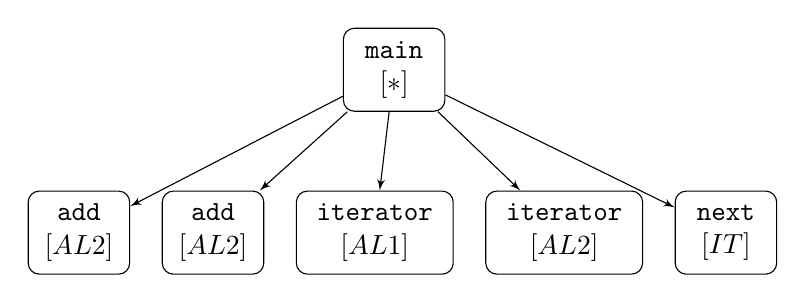
\begin{tikzpicture}
    \node [block] (main) {{\tt main}\\$[*]$};
    \node [block, below left=1cm and 2.7cm of main] (add1) {{\tt add}\\$[AL2]$};
    \node [block, right=0.4cm of add1] (add2) {{\tt add}\\$[AL2]$};
    \node [block2, right=0.4cm of add2] (iterator1) {{\tt iterator}\\ $[AL1]$};
    \node [block2, right=0.4cm of iterator1] (iterator2) {{\tt iterator}\\$[AL2]$};
    \node [block, right=0.4cm of iterator2] (next) {{\tt next}\\$[IT]$};

    \path [line] (main) -- (add1);
    \path [line] (main) -- (add2);
    \path [line] (main) -- (iterator1);
    \path [line] (main) -- (iterator2);
    \path [line] (main) -- (next);

\end{tikzpicture}
}
\end{center}
\caption{Call-graph by $1$-object-sensitive analysis}
\label{fig:obj:callgraph}
\end{subfigure}
\vfill\null
\columnbreak
\begin{subfigure}[b]{.9\columnwidth}
\begin{center}
\resizebox{\columnwidth}{!}{
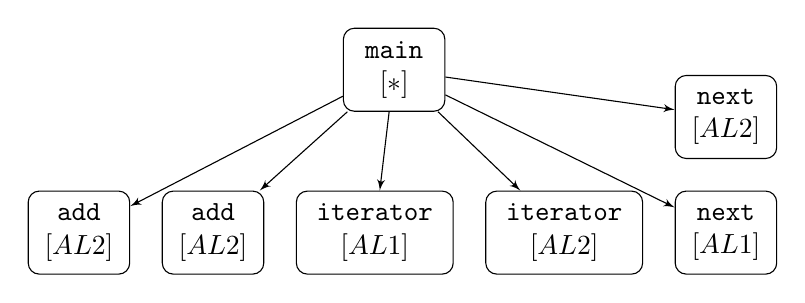
\begin{tikzpicture}
    \node [block] (main) {\tt main\\$[*]$};
    \node [block, below left=1cm and 2.7cm of main] (add1) {{\tt add}\\$[AL2]$};
    \node [block, right=0.4cm of add1] (add2) {\tt add\\$[AL2]$};
    \node [block2, right=0.4cm of add2] (iterator1) {\tt iterator\\$[AL1]$};
    \node [block2, right=0.4cm of iterator1] (iterator2) {\tt iterator\\$[AL2]$};
    \node [block, right=0.4cm of iterator2] (next1) {\tt next\\$[AL1]$};
    \node [block, above=0.4cm of next1] (next2) {\tt next\\$[AL2]$};

    \path [line] (main) -- (add1);
    \path [line] (main) -- (add2);
    \path [line] (main) -- (iterator1);
    \path [line] (main) -- (iterator2);
    \path [line] (main) -- (next1);
    \path [line] (main) -- (next2);

\end{tikzpicture}
}

\end{center}
\caption{Call-graph by $1$-object-sensitive analysis with tunneling}
\label{fig:obj:tunneling}
\end{subfigure}
\end{multicols}
\setlength{\abovecaptionskip}{-5pt}
\caption{Example code and callgraphs}
\label{fig:overviewObj}
\end{figure}

\myparagraph{Example Code for Object Sensitivity}
Example code in Fig.~\ref{fig:obj:code} present common pattern that 1-object-sensitive+heap
analysis lose precision. The main method use two data structure Arraylist, and it add
different data to each Arraylist. Main method makes iterator for each Arraylist and 
get data with iterators. The queries ask if two type casts at line 13 and 14 are
safe. 1-object-sensitive+heap analysis fails to prove the queries because
\texttt{next} method invoked in 13 and 14 are merged as
the method invocations have same context \texttt{IT}, 
constructing call-graph in Fig.~\ref{fig:obj:callgraph}. 

\myparagraph{Context Tunneling for Object sensitivity} 
With context tunneling, 1-object-sensitive+heap analysis can prove the queries. Note that Object sensitivity
has different flavor from call-site sensitivity; it updates context from heap context. Base
variable \texttt{it1} and \texttt{it2} point to same heap allocation but have different heap context: 
\texttt{AL1} and \texttt{AL2}. Applying context tunneling for \texttt{next} method make method call
at line 13 have context \texttt{AL1} and 14 have context \texttt{AL2},
resulting context sensitive analysis prove the queries with call-graph 
Fig.~\ref{fig:obj:tunneling}. 


%%% Local Variables:
%%% mode: latex
%%% TeX-master: "paper"
%%% End:

%\lstset{
%  language=Java,
%  aboveskip=3mm,
%  belowskip=3mm,
%  showstringspaces=false,
%  columns=flexible,
%  basicstyle={\scriptsize\ttfamily},
%  numbers=left,
%  numbersep=5pt,
%  numberstyle=\small\color{gray},
%  keywordstyle=\color{blue},
%  commentstyle=\color{dkgreen},
%  stringstyle=\color{mauve},
%  breaklines=true,
%  breakatwhitespace=true,
%  tabsize=3
%}
%\begin{figure}
%\begin{subfigure}[b]{0.9\columnwidth}
%\begin{multicols}{2}
%\centering
%\begin{lstlisting}
%class A {} class B {}
%class C {
%  public static void main (){
%    ArrayList al1 = new ArrayList();//AL1
%    ArrayList al2 = new ArrayList();//AL2
%
%    al1.add(new A());
%    al2.add(new B());
%
%    ArrayList.ListItr it1 = al1.iterator();
%    ArrayList.ListItr it2 = al2.iterator();
%
%    A a = (A)it1.next();  //Query 1
%    B b = (B)it2.next();  //Query 2
%  }
%}
%
%class ArrayList{
%  Object[] elementData = new Object[10];
%  int size = 0;
%  void add(Object e){
%    elementData[size++] = e;
%  }
%  ListItr iterator(){
%    return new ListItr(); //IT
%  }
%  class ListItr{
%    int cursor = 0;
%    Object next(){
%      return elementData[cursor++];
%    }
%  }
%}
%\end{lstlisting}
%\end{multicols}
%\caption{Example code}
%\label{fig:obj:code}
%\end{subfigure}
%\begin{multicols}{2}
%\begin{subfigure}[b]{.9\columnwidth}
%\begin{center}
%\resizebox{\columnwidth}{!}{
%\begin{tikzpicture}
%    \node [block] (main) {{\tt main}\\$[\cdot]$};
%    \node [block, below left=1cm and 2.7cm of main] (add1) {{\tt add}\\$[AL1]$};
%    \node [block, right=0.4cm of add1] (add2) {{\tt add}\\$[AL2]$};
%    \node [block2, right=0.4cm of add2] (iterator1) {{\tt iterator}\\ $[AL1]$};
%    \node [block2, right=0.4cm of iterator1] (iterator2) {{\tt iterator}\\$[AL2]$};
%    \node [block, right=0.4cm of iterator2] (next) {{\tt next}\\$[IT]$};
%
%    \path [line] (main) -- (add1);
%    \path [line] (main) -- (add2);
%    \path [line] (main) -- (iterator1);
%    \path [line] (main) -- (iterator2);
%    \path [line] (main) -- (next);
%
%\end{tikzpicture}
%}
%\end{center}
%\caption{Call-graph by $1$-object-sensitive analysis}
%\label{fig:obj:callgraph}
%\end{subfigure}
%\vfill\null
%\columnbreak
%\begin{subfigure}[b]{.9\columnwidth}
%\begin{center}
%\resizebox{\columnwidth}{!}{
%\begin{tikzpicture}
%    \node [block] (main) {\tt main\\$[\cdot]$};
%    \node [block, below left=1cm and 2.7cm of main] (add1) {{\tt add}\\$[AL1]$};
%    \node [block, right=0.4cm of add1] (add2) {\tt add\\$[AL2]$};
%    \node [block2, right=0.4cm of add2] (iterator1) {\tt iterator\\$[AL1]$};
%    \node [block2, right=0.4cm of iterator1] (iterator2) {\tt iterator\\$[AL2]$};
%    \node [block, right=0.4cm of iterator2] (next1) {\tt next\\$[AL1]$};
%    \node [block, above=0.4cm of next1] (next2) {\tt next\\$[AL2]$};
%
%    \path [line] (main) -- (add1);
%    \path [line] (main) -- (add2);
%    \path [line] (main) -- (iterator1);
%    \path [line] (main) -- (iterator2);
%    \path [line] (main) -- (next1);
%    \path [line] (main) -- (next2);
%
%\end{tikzpicture}
%}
%
%\end{center}
%\caption{Call-graph by $1$-object-sensitive analysis with tunneling}
%\label{fig:obj:tunneling}
%\end{subfigure}
%\end{multicols}
%\setlength{\abovecaptionskip}{-5pt}
%\caption{Example and call-graphs constructed by the conventional 1-object-sensitivity and our
%1-object-sensitivity with context tunneling}
%\label{fig:overviewObj}
%\end{figure}
%
%\myparagraph{Example Code}
%
%Fig.~\ref{fig:obj:code} shows
%a common code pattern that $1$-object-sensitivity with a context-sensitive heap
%loses precision, which is found frequently in data
%structure implementations such as List and Map.
%In the example code, we have four
%top-level classes, \texttt{A}, \texttt{B}, \texttt{C}, and
%\texttt{ArrayList}, and an inner class \texttt{ListIter} inside of the
%\texttt{ArrayList} class. The \texttt{ArrayList} class % , as the name suggests,
%% models on \texttt{java.util.ArrayList}, which is
%implements a resizable array.
%For simplicity, it maintains data in the % (fixed-size)
%\texttt{elementData} array and has the \texttt{add} method to append new data at
%the end of \texttt{elementData}. It also has the \texttt{iterator} method that
%returns an object of type \texttt{ListIter}, providing access to \texttt{elementData}.
%The \texttt{main} method in class \texttt{C} performs usual
%allocate-add-retrieve
%tasks using \texttt{ListIter}. The goal of the pointer
%analysis is to prove the safety of two type casts at lines 13
%and 14.
%
%\myparagraph{Conventional Object-Sensitivity}
%
%Conventional object-sensitivity analyzes different method calls
%separately for their base objects (and their heap contexts, if needed)~\cite{Smaragdakis2011}.  For
%example, when we analyze the \texttt{next} method at line 13,
%2-object-sensitivity creates the context $[\texttt{AL1},
%\texttt{IT}]$, where \texttt{IT} is the allocation-site of the base
%object (\texttt{it1}) and \texttt{AL1} is its heap context.
%Likewise, the
%method invocation at line 14 creates the context $[\texttt{AL2}, \texttt{IT}]$, enabling
%the analysis to distinguish the first and second calls to the same method. Using base objects
%as contexts makes object-sensitivity more favorable than
%call-site-sensitivity for object-oriented languages. However, it still
%updates contexts unconditionally at every method call and may lose important
%context elements when $k$ is not sufficiently large. For example, when we
%analyze the code with 1-object-sensitivity, the two calls to
%\texttt{next} are analyzed under the same context $[\texttt{IT}]$
%(Fig.~\ref{fig:obj:callgraph}).
%As a result, both objects \texttt{A} and \texttt{B} get returned to both
%queries simultaneously, making the analysis fail to prove the safety of type
%casting.
%
%
%
%\myparagraph{Object-Sensitivity with Context Tunneling}
%With context tunneling, however, even 1-object-sensitivity can prove the queries. Note that
%object-sensitivity has a different flavor from call-site-sensitivity; it
%updates the context with the heap context of the base object~\cite{Milanova2005, Milanova2002}. Base
%variables \texttt{it1} and \texttt{it2} point to the same heap allocation with different heap contexts: \texttt{AL1} and \texttt{AL2}. Applying context
%tunneling for the two method calls to \texttt{next} corresponds to
%propagating the heap contexts \texttt{AL1} and \texttt{AL2} at lines
%13 and 14, respectively, without modification.
%% makes the method call at line 13 to have
%% the context \texttt{AL1} and the method call at 14 to have the context \texttt{AL2}.
%The resulting context-sensitive analysis proves the queries with a call-graph
%shown in Fig.~\ref{fig:obj:tunneling}.


%%% Local Variables:
%%% mode: latex
%%% TeX-master: "paper"
%%% End:

%\newpage

\section{Pointer Analysis with Context Tunneling} \label{sec:tunneling}
Now, we formally describe the idea of context tunneling on the top the analysis rule in Figure~\ref{pre:baseline-rules}.
%\subsection{Analysis with Context Tunneling}\label{sec:tunneling-analysis}
%Now we describe context tunneling on top of the generic context-sensitive analysis.
We assume that a binary relation $\TunnelingRelation$ on methods,
called tunneling relation, is given prior to the analysis:
% The idea of tunneling is simple: compare the
% parent and child contexts and use the more important one as the
% calling context of the called method.  We do so by using a binary
% relation
% $\TunnelingRelation$ on methods, called tunneling relation:
\[
  \TunnelingRelation \subseteq \Methods \times \Methods.
\]
Intuitively, $\TunnelingRelation$ relates the parent and child methods
that require context tunneling. Suppose that a method
$m_2$ is called during analysis where its parent method is $m_1$. If
$m_1$ and $m_2$ are related by $\TunnelingRelation$, i.e., $(m_1,m_2) \in \TunnelingRelation$, we apply context tunneling by
reusing the context of the parent method ($m_1$) in analyzing the
child method ($m_2$) without creating a new context for $m_2$.  Given
a tunneling relation $\TunnelingRelation$, the analysis rule for
performing context tunneling is defined in
Figure~\ref{fig:tunneling-rules}. All the existing rules except for
method calls are carried over to the new analysis without any modifications.
The rule for method call in Figure~\ref{pre:baseline-rules} is
replaced by the rule in Figure~\ref{fig:tunneling-rules}, where the
only difference is in the way of constructing the child context
$\ctx'$. If $(p,m) \not\in \TunnelingRelation$ (i.e. tunneling
disabled), we update the calling context as the conventional $k$-context-sensitive
analysis does. Otherwise, when $(p,m)\in \TunnelingRelation$
(i.e. tunneling enabled), we just pass the parent context $\pctx$ to
the child method (i.e. $\ctx' = \pctx$) without appending the current
context element to $\pctx$.
% Note that the ordinary $k$-context-sensitive analysis and
% context-insensitive analysis are special cases with
% $\TunnelingRelation = \emptyset$ and
% $\TunnelingRelation = \Methods \times \Methods$, respectively.


Although the idea of context tunneling is simple, realizing effective
tunneling in practice is challenging. We found that the performance of
context tunneling is very sensitive to the choice of the tunneling
relation; with a good relation, context tunneling is able to improve the
baseline analysis significantly but, with an inappropriate choice, the analysis
becomes even inferior to the context-insensitive analysis.  Manually finding a general heuristic rule to
generate an optimal tunneling relation for a given program was
difficult for real-world Java programs.
The goal of Section~\ref{tunneling:learning} is to address this challenge
with a data-driven technique that automatically learns a good
tunneling heuristic from data.

\begin{figure}[t]
  \[
    \begin{array}{c}
      \infer[]
      {
      \begin{array}{c}
        \ctx' \in \Reachable ({m}) \quad
        ({\heap}, {\hctx}) \in  \VarPointsTo ({m_{\this}}, {\ctx'}) \\
        \VarPointsTo({\it arg}, \ctx) \subseteq \VarPointsTo(m_{\it param}, \ctx')
        \quad
        \VarPointsTo(m_{\it return}, \ctx') \subseteq \VarPointsTo(x, \ctx)\\
        (\invo, \ctx, m, \ctx') \in \CallGraph
      \end{array}
      }{
      \begin{array}{c}
        {\it \invo : x = y.\sig({\it arg})} \quad
        \ctx \in    \Reachable ({\methof(\invo)}) \\
        ({\heap}, {\hctx})\in  \VarPointsTo ({\it y},\ctx) \quad
        t = {\typeof}(\heap)  \quad m = {\lookup}(t, \sig) \\
(e, {\pctx}, p) = \parent(\heap,\hctx, \invo, \ctx) \quad
        \ctx' = \left\{
        \begin{array}{l@{\quad}l}
          \truncateCtx{\appendCtx{{ \pctx}}{{e}}}{\CallDepth}
          & \mbox{if}~(p,m)\not\in \TunnelingRelation \\
          \truncateCtx{\pctx}{\CallDepth}     & \mbox{if}~(p,m)
                                                \in \TunnelingRelation
        \end{array}
                                                          \right.
      \end{array}
                                                          }
    \end{array}
  \]
  \caption{Context-sensitive pointer analysis with tunneling}
\label{fig:tunneling-rules}
\end{figure}

%%% Local Variables:
%%% mode: latex
%%% TeX-master: "paper"
%%% End:

\section{Learning Context-Tunneling Heuristics}\label{tunneling:learning}

Now, we present a machine-learning algorithm specialized for
generating good context tunneling heuristics from a dataset
of programs.


 % Although the
% idea of context tunneling is simple, realizing effective tunneling in
% practice is challenging. The performance of context tunneling depends
% on the choice of the tunneling relation $\TunnelingRelation$, but
% manually designing a heuristic rule to generate $\TunnelingRelation$
% for a given program is nontrivial and likely ends up with costly or
% imprecise results.  Our goal is to address this challenge by
% developing a machine-learning algorithm that learns
% context-tunneling heuristics from data.


\subsection{Parametric Program Analysis} \label{tunneling:setting}

Let us first encapsulate our analysis in Section~\ref{sec:tunneling}
as a parametric program analysis~\cite{Liang2011learning}.  Let
$P \in \Program$ be a program to analyze. Let $\Methods_P$ be the set
of methods in $P$.  Then, we can define the set $\tspace_P$ of all
tunneling relations for $P$ as follows:
\[
 \TunnelingRelation \in \tspace_P = \power{\Methods_P \times \Methods_P}.
\]
The set $\tspace_P$ forms the parameter space of the analysis for $P$,
where an element $\TunnelingRelation \in \tspace_P$ --- a set of
method pairs --- represents a tunneling relation.  Abstractions are
ordered by set inclusion.  For each pair $(m_1,m_2)$ of parent and
child methods in $\TunnelingRelation$, we apply context-tunneling by
reusing the calling context of the parent method ($m_1$) when analyzing the
child method ($m_2$) without creating a new context for $m_2$.  The abstraction
space covers the conventional context-insensitive and -sensitive
analyses: with $\TunnelingRelation = \emptyset$, the analysis becomes
an ordinary $k$-context-sensitive analysis, and with
$\TunnelingRelation = \Methods_P \times \Methods_P$, the analysis
equals to the context-insensitive analysis.

We assume that a set $\Assertion_P$ of assertions is given together
with the input program $P$.  For instance, $\Assertion_P$ may denote the set of all type casts in
$P$ and the analysis attempts to prove that they do not fail at
runtime (i.e. no down-casting failures).  Then,
we can model pointer analysis for $P$ by the function $F_P$:
\[
  F_P \in \tspace_P \to \power{\Assertion_P} \times \mbn.
\]
Given a program $P$ and a tunneling relation
$\TunnelingRelation \in \tspace_P$, $F_P(\TunnelingRelation)$ returns
the set $Q \subseteq \Assertion_P$ of proved assertions and the
analysis time $n \in \mbn$ represented by a natural number (e.g. time
took to analyze the program).  We define two projection functions:
$\proved(F_P(\TunnelingRelation))$ and
$\cost(F_P(\TunnelingRelation))$ denote the set of proved assertions
($Q$) and the analysis cost ($n$) of the analysis
$F_P(\TunnelingRelation)$, respectively.

% Once $\heuristic$ is generated, it can be used to analyze previously
% unseen program $P$ with $F_P (\heuristic(P))$.  We aim to learn a
% tunneling heuristic $\heuristic$ such that the analysis
% $F_P(\heuristic(P))$ improves the precision as much as possible while
% retaining the cost of the baseline analysis
% $F_P(\emptyset)$ (i.e. the ordinary $k$-context-sensitive analysis).

\myparagraph{Non-Monotonicity}

One noticeable property of context tunneling is non-monotonicity.  Note
that existing parametric program analyses are typically monotone with respect to
their parameters; that is, the analysis precision is monotonically
increasing (or decreasing) with respect to the parameters of the
analysis
(e.g.~\cite{Liang2011learning,JeJeChOh17,Zhang2014,Liang2011}).  That
is, if $p \sqsubseteq p'$ then
$\proved(F_P(p)) \subseteq \proved(F_P(p'))$ (or
$\proved(F_P(p)) \supseteq \proved(F_P(p'))$). For example, in a
selective context-sensitive analysis~\cite{JeJeChOh17}, making more
methods context-sensitive always increases precision.  In our case,
however, the analysis is not monotone with respect to the parameters
(i.e. context-tunneling relations). That is,
$\TunnelingRelation \subseteq \TunnelingRelation'$ does not imply
$F_P(\TunnelingRelation) \subseteq F_P(\TunnelingRelation')$ or
$F_P(\TunnelingRelation) \supseteq F_P(\TunnelingRelation')$.  Consequently, neither $F_P(\emptyset)$ nor
$F_P(\Methods_P\times\Methods_P)$ --- the conventional
$k$-context-sensitive analysis and context-insensitive analysis --- is
the most precise one in the parameter space of context tunneling.
As we describe in
Section~\ref{tunneling:learning-algorithm}, this unusual property makes
learning challenging; in particular, we cannot use the existing
learning algorithms (e.g.~\cite{JeJeChOh17,Liang2011learning}) that
exploit the monotonicity of analysis.


\subsection{Machine-Learning Model for Context Tunneling}


%\myparagraph{Parameterized Heuristic}

Our goal is to learn a {\em tunneling heuristic}, denoted
$\heuristic$, from a dataset of programs, which takes a program $P$
and returns a tunneling relation for $P$:
\[
  \heuristic(P) \in \power{\Methods_P \times \Methods_P}.
\]
To generate such a heuristic automatically, we need to define a space
of possible tunneling heuristics, called model or inductive bias in
the machine learning community.  A standard
method is to define the space by a generic heuristic with free
parameters, reducing the problem of generating a good heuristic to the
problem of finding appropriate parameter values.  There is a number of
different ways to define such a parameterized heuristic. For example,
we can use a linear combination of input features~\cite{Oh2015} or a
non-linear, disjunctive combination~\cite{JeJeChOh17}. We take the latter approach because the
non-linear method is known to be more effective for pointer analysis
than the simple linear approach~\cite{JeJeChOh17}.

Following \cite{JeJeChOh17},
we use a boolean formula over atomic features as a model parameter.
Let us assume that a set of {\em atomic features} is given:
$\afeatures = \myset{\afeat_1, \afeat_2, \dots, \afeat_n}$, where a feature $\afeat_i$ describes a property of
methods. It is a function from programs to predicates on
methods:
\[
\afeat_i(P) : \Methods_P \to \myset{\true,\false}.
\]
For example, a feature may express the set of methods that have
heap allocation in their bodies. We shortly present our atomic features in
detail.
Given a set of atomic features, we can express more complex features
of methods by combining the atomic features.
We combine them with
a boolean formula $f$ in disjunctive normal form, i.e., a disjunction of conjunctions
of literals:
\[
f = \bigvee_i \bigwedge_j l_{i,j}
\]
where $l_{i,j}$ is a literal: $\true$, $\false$, atomic feature $a \in \afeatures$,
or their negations.
Note that the meaning of a boolean formula is a set of methods.
Given a program $P$ and a formula $f =\bigvee_i \bigwedge_j l_{i,j}$, let $\sem{f}_P$ be the set of methods
on which the formula $f$ evaluates to true: $\sem{f}_P = \bigcup_i
\bigcap_j \sem{l_{i,j}}_P$ where $\sem{\true}_P = \Methods_P$,
$\sem{\false}_P = \emptyset$, $\sem{\afeat_i}_P = \myset{m \in
 \Methods_P \mid \afeat_i(P)(m) = \true}$, and $\sem{\neg a_i}_P =
 \Methods_P \setminus \sem{a_i}_P$.
In the rest of this chapter, we often represent a formula in
disjunctive normal form by a set of sets of literals. For example, the formula
$f = (a_1 \land a_2) \vee (\neg a_3 \land a_4)$ can be
represented by $\myset{\myset{a_1,a_2}, \myset{\neg a_3,a_4}}$.



Our model uses two boolean formulas $\params = \langle f_1,f_2
\rangle$ and generates the tunneling relation for a given program $P$ as follows:
\begin{equation}\label{eq:heuristic}
\heuristic_{\params} (P) = \myset{(m_1,m_2) \in \Methods_P \times
  \Methods_P \mid
  m_1 \in \sem{f_1}_P \vee m_2 \in \sem{f_2}_P}.
\end{equation}
The generated relation includes a pair $(m_1, m_2)$ of methods if
$m_1 \in \sem{f_1}_P$ or $m_2 \in \sem{f_2}_P$.
This conditions says that we apply context tunneling when
$m_1$ is implied by $f_1$ or $m_2$ by $f_2$. Intuitively, $f_1$ denotes the set of methods that improve the
analysis performance by passing their contexts to child methods, and
$f_2$ describes the methods that benefit by reusing the contexts of
their parent methods. The goal of our learning algorithm is to
discover the characteristics of such methods, represented by boolean
combinations ($f_1$ and $f_2$) of features, that maximize the performance of
the heuristic.

\begin{table}[t]
     \centering	\scriptsize
    \caption{Atomic features used in evaluation}
    \label{tbl:features}
\begin{tabular}{c}
    \begin{tabular}{clcclcclcclccl}
        \toprule
        \multicolumn{14}{c}{Class A (Signature features)} \\
        \midrule
        A1 & ``java'' &\quad& A2 & ``lang'' &\quad& A3 & ``sun'' &\quad& A4 & ``()'' &\quad& A5 & ``void'' \\
        A6 & ``security'' &\quad& A7 & ``int''  &\quad&  A8 & ``util'' &\quad& A9 & ``String'' &\quad&  A10 & ``init'' \\
        \bottomrule
    \end{tabular}
%\quad
%	\begin{tabular}{clclcl}
%		\toprule
%		\multicolumn{6}{c}{Class B (Statement features)} \\
%		\cmidrule(lr){1-6}
%		 B1 & Assign & B6 &
%		Breakpoint & B11 & Lookup \\
%		 B2 & Identity & B7 &
%		EnterMonitor & B12 & Nop \\
%		 B3 & Invoke & B8 &
%		ExitMonitor & B13 & Ret \\
%		 B4 & Return & B9 &
%		Goto & B14 & ReturnVoid \\
%		 B5 & Throw & B10 &
%		If & B15 & TableSwitch \\
%		\bottomrule
%	\end{tabular}
\\
\\
    \begin{tabular}{clcl}
        \toprule
        \multicolumn{4}{c}{Class B (Additional features)} \\
        \midrule
%          B1 & Methods contained in nested class  			& B8 & Methods containing virtual method invocation\\
% B2 & Methods taking multiple arguments 			& B9 & Static method \\
% B3 & Methods containing array load 				& B10 & Methods containing a single heap allocation \\
% B4 & Methods containing local assignments 			& B11 & Methods taking an argument of Object type \\
% B5 & Methods containing local variables 			& B12 & Methods containing multiple heap allocations \\
% B6 & Methods containing field store 				& B13 & Methods contained in a large class\\
% B7 & Methods containing static method invocation\\

 B1 & Methods contained in nested class  			& B7 & Methods containing static method invocation\\
 B2 & Methods taking multiple arguments 			& B8 & Methods containing virtual method invocation\\
 B3 & Methods containing array load 				& B9 & Static method \\
 B4 & Methods containing local assignments 			& B10 & Methods containing a single heap allocation \\
 B5 & Methods containing local variables 			& B11 & Methods taking an argument of Object type \\
 B6 & Methods containing field store 				& B12 & Methods containing multiple heap allocations \\
 & & B13 & Methods contained in a large class\\

      %    \#11 & Methods contained in inner class\\
      %    \#12 & Methods taking multiple arguments\\
      %   \#13 & Methods containing array load \\ % \textsc{LoadArrayIndex}
      %   % instruction\\
      %    \#14 & Methods containing local assignments \hakjoo{what is
      %           ``local assignment''?}\\
      %    \#15 & Methods containing local variables \\
      %    \#16 & Methods containing field store\\ % \textsc{StoreInstanceField} instruction\\
      %    \#17 & Methods containing static method invocation\\
      %    \#18 & Methods containing virtual method invocation\\
      %    \#19 & Methods containing a single heap allocation%  \hakjoo{single heap
      %           % alloc?} \\ &\minseok{yes only one heap allocation}
      % \\
      %    \#20 & Methods taking an argument of the ``Object'' type \\
      %    \#21 & Methods containing multiple heap allocations%  \hakjoo{diff with
      %           % \#19?}\\ &\minseok{Yes, 19 $\subset$ 21}
      % \\
      %    \#22 & Methods contained in a large class (\#Methods~$>$~20) \\
      %    \#23 & Static methods \\
        \bottomrule
    \end{tabular}
\end{tabular}
\end{table}


\myparagraph{Atomic Features}\label{sec:features}

Table~\ref{tbl:features} shows 23 atomic features we have used in learning.
Each feature in Table~\ref{tbl:features} describes a syntactic
property of Java method definitions.  The features are classified into
two types: signature features (Class A) and additional
features (Class B).  Signature features (A1 -- A10) came from the existing work~\cite{JeJeChOh17} and
additional features (B1 -- B13) have been newly designed in this work.
Signature features consist of strings that most frequently appear in
method signatures from the DaCapo suite~\cite{Blackburn2006}. For example, the feature A5
(``void'') denotes the set of methods whose signature strings include
``void'' as a substring.  On the
other hand, features B1 -- B13 describe slightly higher-level
properties.  For example, the feature B1 denotes the set of methods
that belong to inner classes.
When choosing atomic features, we focused on collecting as many simple
features as possible and let the learning algorithm to discover
meaningful combinations of them automatically. In Section~\ref{sec:eval:algorithm}, we discuss impact of
using different atomic features.
%
%C3 Methods containing array load:\\
%Load value from array to a local variable\\
%
%C4 Methods containing local assignment:\\
%Local variable to local variable assignment\\
%
%C6 Methods containing field store:\\
%Store value from a local variable to instance's field

% Simply
% combining the signature and statement features is not able to describe
% such a property.

\subsection{Optimization Problem}\label{sec:opt}
Formally, the learning problem is expressed as an optimization
problem.
Given program analysis $F$, parameterized heuristic
$\heuristic_{\params}$ defined in (\ref{eq:heuristic}), and  training programs
$\vec{P} = \myset{P_1,\dots,P_m}$,
our goal is to find the parameters $f_1$ and $f_2$ that maximize the
precision of the analysis over the codebase:
\[
  \mbox{Find $\params = \langle f_1, f_2 \rangle$ that maximizes} \sum_{P \in \vec{P}}
  |\proved(F_{P}( \heuristic_{\params}(P)))|
\]
such that $\params = \langle f_1,f_2 \rangle$ satisfies the following constraint on
the analysis cost:
\[
\sum_{P \in \vec{P}} \cost(F_P(\heuristic_{\params}(P) )) \le \sum_{P \in \vec{P}} \cost(F_P(\emptyset)).
\]
The constraint says that the analysis with context tunneling ($F_P(\heuristic_\params(P))$) is at
least as scalable as the baseline analysis
without tunneling ($F_P(\emptyset)$).



\subsection{Learning Algorithm}\label{tunneling:learning-algorithm}
Now, we present an algorithm that effectively solves the
optimization problem.  The key challenge, which makes our algorithm
substantially differ from the existing learning
algorithms~\cite{Liang2011learning,JeJeChOh17}, is that the analysis
$F$ is not monotone with respect to the tunneling relations.  In
existing learning algorithms~\cite{Liang2011learning,JeJeChOh17},
monotonicity plays a central role in finding analysis parameters
efficiently. They start from the most precise abstraction, and
iteratively refine the abstraction until a smallest abstraction that
satisfies a given constraint is found; here monotonicity allows the
algorithms to safely rule out a large set of abstractions smaller than any
previously failed (constraint-unsatisfying)
abstractions. Consequently, these algorithms follow a (decreasing)
chain of parameters and monotonicity ensures that this strategy
is optimal. However,
when the analysis is not monotone, simply following a chain of
parameters no longer provides such a guarantee.
Our algorithm is able to find a
good parameter over the non-monotonic space of tunneling relations by
exploring the search space in a non-greedy way that seeks to
maximize the final benefit, instead of the immediate benefit.

% however, we do not know the most precise abstraction from which the
% refinement process should start.  This unusual property makes
% learning challenging; in particular, we cannot use the existing
% algorithm~\cite{JeJeChOh17} that gradually refines parameters in a
% ``greedy'' fashion by exploiting the monotonicity of the analysis.

% Our algorithm is able to find a
% good parameter over the non-monotonic space of tunneling relations.
% The most important distinguishing feature, compared to the existing
% learning algorithms~\cite{JeJeChOh17,Liang2011learning}, is that our
% algorithm explores the search space in a non-greedy way that seeks to
% maximize the final benefit, instead of the immediate benefit.  % Our
% algorithm keeps refining parameters as long as they have potential in
% the long run even though doing so immediately decreases the analysis
% precision.
%\hakjoo{Clarify the challenge and the key idea.}

\myparagraph{Overall Algorithm}

The overall algorithm consists of two phases.  It first learns the
formula $f_2$, aiming at characterizing the methods that increase the
analysis precision by inheriting contexts from their parent methods
instead of creating their own ones.  With the learned $f_2$, the
algorithm continues to learn $f_1$, the set of methods that improves
the precision by passing their contexts to child methods. Those two
formulas $f_1$ and $f_2$ become the parameter
$\params = \langle f_1, f_2 \rangle$ of the heuristic
$\heuristic_\params$.  Procedure \textsc{Learn} in
Algorithm~\ref{alg:overall} describes the overall procedure. It
takes three inputs: a static analyzer $F$ parameterized by tunneling
relations, a set $\vec{P}$ of training programs, and a set
$\afeatures$ of atomic features. The algorithm calls the same
subroutine, \LearnBooleanFormula, twice with different
parameters. Note that the formula $f_2$ learned in the first phase is
used in the second phase at line 3.
In the rest of this section, we write $\params(i)$ when $\params =
\langle f_1, f_2\rangle$ for $f_1$ (when $i = 1$) or $f_2$ (when $i=2$), and write
$\params[f_i \mapsto g]$ for $\langle g, f_2\rangle$ (when $i=1$) or $\langle
f_1, g\rangle$ (when $i=2$).

\begin{algorithm}[t]
  \caption{Overall Algorithm}\label{alg:overall}\small
  \begin{algorithmic}[1]

    \Require Static analyzer $F$, codebase $\vec{P}$, atomic features
    $\afeatures$ \Ensure Model parameters $f_1$ and $f_2$
    \Procedure{Learn}{$F$, $\vec{P}$, $\afeatures$} \State
    $f_2 \gets \LearnBooleanFormula(2, \false, F, \vec{P},
    \afeatures)$ \Comment{learn methods for child contexts} \State
    $f_1 \gets \LearnBooleanFormula(1, f_2, F, \vec{P}, \afeatures)$
    \Comment{learn methods for parent contexts} \State \Return
    $\langle f_1, f_2 \rangle$
    \EndProcedure
\end{algorithmic}
\end{algorithm}

\begin{algorithm}[t!]
  \caption{Learning a Single Parameter}\label{alg:learning}\small
  \begin{algorithmic}[1]
		\Require Index $i$ of parameter to learn, parameter $f_2$, static analyzer $F$, codebase $\vec{P}$,
		atomic features $\afeatures$
		\Ensure $i^{\it th}$ parameter $f_i$
		\Procedure{\LearnBooleanFormula}{$i, f_2, F, \vec{P},
                  \afeatures$}
\State $f_1 \gets \false$

%\For{$i=2$ \textbf{to} $1$} \Comment{learn $f_2$ and then $f_1$}

                % \State $f_1 \gets \false$
		 \State $\params \gets \langle f_1, f_2 \rangle$
%                \Comment{initial parameter}
                \State $W \gets \myset{a \in (\afeatures \cup \neg \afeatures) \mid
\SeedFeature (a, i, \params, F, \vec{P})}$ \Comment{collect seed features}

 % \CollectSeedFeatures (i,\params,F,
 %                \vec{P}, \afeatures) $

		\While {$W \neq \emptyset$}
		  \State $s \gets \ChooseSeed(i,\params,F,\vec{P},W)$
                  \Comment{pick a seed feature from $W$ with highest potential}
		  \State $W \gets W \setminus \myset{s}$
		  \State $c \gets \RefineSeed(s, i,\params,
                  \afeatures, F, \vec{P})$ \Comment{refine seed
                    feature $s$}


		  \State $\params' \gets \params[f_i \mapsto f_i \vee c]$ \Comment{new parameter to be evaluated}
		  \If {$\GoodHeuristicFound(\params, \params',
                    \vec{P})$}\Comment{check whether new parameter
                    improves }
%		    \State $f_i \gets f_i \ \vee {c}$ \Comment{update parameter}
  		    \State $\params \gets \params'$ \Comment{update parameter}
		  \EndIf
		\EndWhile
%\EndFor
		\State \Return $\params(i)$ \Comment{return $f_i$}
		\EndProcedure
\end{algorithmic}
\end{algorithm}

\begin{algorithm}[t!]
  \caption{Refining a Seed Feature}\label{alg:refine}\small
  \begin{algorithmic}[1]
		\Require Seed feature $s$, parameter index $i$,
                parameters $\params$, atomic features $\afeatures$, static analyzer $F$, codebase $\vec{P}$
		\Ensure refined conjunction $c$

    \Procedure{\RefineSeed}{$s$, $i$, $\params$, $\afeatures$, $F$, $\vec{P}$}
    \State $c \gets s$\Comment{initial conjunction}
          \State $\Failed \gets \emptyset$ \Comment{$\Failed$ will
            maintain features that fail to refine $c$}

		  \While {$(a \gets \ChooseAtom(\afeatures,f_i,
                    c,\vec{P},\Failed)) \not= \false$}  \Comment{iteratively refine conjunction $c$}
%                  \State $a \gets \ChooseAtom(\afeatures,f_i,
%                    c,\vec{P},\Failed)$
   	        \State $c' \gets c \land {a}$ \Comment{refine $c$ with $a$}

  	        \State $\params' \gets \params[f_i \mapsto f_i\vee c]$ \Comment{old parameter}
  	        \State $\params'' \gets \params[f_i \mapsto f_i\vee
                c']$ \label{alg:if}\Comment{new (refined) parameter}
  	        \If {$\PrecP(\params', \params'', \vec{P}) \wedge
                  \HasSeed(\params'', \params, \vec{P})$}
\Comment{precision improved}
  	          \State $c \gets c'$
  	        \ElsIf{$\PrecE(\params', \params'', \vec{P}) \wedge
                  \CostM(\params', \params'', \vec{P})$}
\Comment{cost reduced without precision loss}
  	          \State $c \gets c'$
            \Else
              \State $\Failed \gets \Failed \cup \myset{a}$ \Comment{record failed attempt}
  	        \EndIf
		  \EndWhile
\State \Return $c$
\EndProcedure

	\end{algorithmic}
\end{algorithm}

% \myparagraph{Learning a Boolean formula}

% Informally, our
% algorithm first evaluates each atomic feature's potential as a good
% context tunneling heuristic. We say a atomic feature has a {\it
%   potential} if using the feature as the sole context tunneling
% heuristic proves at least one additional queries that ordinary context
% sensitivity can't. Note that we don't measure an atomic feature's
% potential with the respect to the number of proven queries. Using the
% number of additionally provable queries instead of total provable
% queries enables our algorithm to explore locally bad but globally good
% solutions during a process. From the promising atomic features, our
% algorithm gradually refines the features one by one by repeatedly
% conjoining it with other atomic features. If the conjunction results a
% better heuristic than before, our algorithm accepts the
% change. Otherwise, the algorithm memorizes the failure and repeats the
% conjoining process until the algorithm can't find an atomic feature to
% conjoin with. When the algorithm fully refined an atomic feature, the
% resulting conjunction is evaluated to see if having the conjunction to
% the formula results better precision and performance than before. If
% so, the algorithm updates the formula with the conjunction and repeats
% the process until we have atomic features to refine.

% Then, our learning algorithm outputs a context tunneling heuristic $f_i$ in a Boolean formula in disjunctive of conjunctions of literals that are atomic features and theirs negations. Through out the algorithm, we represent a conjunctive clause by a set of literals (i.e., atomic feature), and a disjunction by a set of clauses.

%\[
%\CollectSeedFeatures(i, \params, F, \afeatures, \vec{P})
%= \myset{a \in \afeatures \mid
%\bigcup_{P \in \vec{P}}\precision(F_P(\heuristic_{\params[f_i \mapsto \myset{\myset{a}}]}(P))) \setminus
%                  \precision(F_P(\heuristic_{\params}(P)))  \neq \emptyset}
%\]

% When learning $f_2$, $\params$ is set to $\langle \false, \false \rangle$, which means a conventional analysis without context tunneling. And, after learning $f_2$, we use it to set an initial parameter for learning $f_1$ in next \textsc{LearnBooleanFormula} invocation. From the initial parameter, the goal of our algorithm is finding two Boolean formulas $f_1$ and $f_2$, one for each $\textsc{LearnBooleanFormula}$ invocation, that maximize precision of analysis while keeping analysis cost as low as the conventional analysis. One of key differences of our work with respect to the~\cite{JeJeChOh17} is a role of the initial parameter. In previous work, the initial parameter determines an upper bound of learned parameters' precision, and the goal of the algorithm is finding the parameter that minimizes the analysis cost while satisfying given precision constraint. In contrary, for the problem of context tunneling, the initial parameter $\params=(\false, \false)$ doesn't mean the most precise heuristic at all; in fact, for the problem of context tunneling, such heuristic is unknown. Therefore, our algorithm uses the initial parameter for two reasons: 1) it provides cost constraint our learned parameters should satisfy; 2) queries proven by the initial parameter become a yardstick to find first set of atomic features our learning algorithm refine to. We explain shortly details of the choice.


%  $W$ of atomic features who
% have tunneling potential with respect to the initial parameter. We say
% an atomic feature has potential if we have at least one unseen proven
% query (i.e., $q \notin \proved(F_P(\heuristic_{\params}(P)))$ where $q
% \in Q_P$) when the atomic feature is used as a sole parameter for
% $f_i$ (i.e., $f_i=\myset{\myset{a}}$) instead of the initial
% parameter. Our intuition behind the concept of potential is that, by
% focusing on the number of unseen proven queries instead of total
% proven queries, we give our algorithm chance to explore locally bad
% but globally good choices during the process. We discuss the effect of
% exploration in Section~\ref{sec:eval:algorithm} in detail. We find
% such atomic features using two functions \CollectSeedFeatures~and
% \HasSeed~with following definitions:

\myparagraph{Learning a Single Parameter}
Procedure \LearnBooleanFormula~in Algorithm~\ref{alg:learning} takes four inputs: index $i$
indicating the formula to learn (i.e. $i=1,2$ when learning $f_1,f_2$,
respectively), learned formula $f_2$ (if any), static analyzer $F$,
training programs $\vec{P}$, and atomic features $\afeatures$.
At line 3, we initialize the parameter
$\params = \langle f_1, f_2 \rangle$, where both $f_1$ and $f_2$ are
$\false$ in the beginning (when we learn $f_2$).  Note that, at this point, the heuristic
$\heuristic_{\params}$ indicates performing the conventional
$k$-context-sensitive analysis without context tunneling.
The goal of the algorithm is to discover a heuristic $\heuristic_{\params'}$
that maximally increases the precision of the baseline analysis
without sacrificing its scalability. Our strategy to do so is to identify what
we call {\em seed features} and iteratively refine them to maximize
their effectiveness.
We say $a \in (\afeatures \cup \neg \afeatures)$ is a seed feature if it describes methods
for which applying context tunneling has potential to improve the
precision of the baseline analysis.
We define the predicate $\SeedFeature$ as follows:
\[
\SeedFeature(a, i, \params, F, \vec{P}) =
\big( \bigcup_{P \in \vec{P}}\precision(F_P(\heuristic_{\params[f_i
  \mapsto a]}(P))) \setminus
                  \precision(F_P(\heuristic_{\params}(P)))\big)
                  \neq \emptyset
\]
In words, $\params$ denotes the current baseline heuristic (e.g. conventional
analysis without tunneling in the beginning).
Let $A = \precision(F_P(\heuristic_{\params}(P)))$ be the set of
queries proved by the baseline analysis. Let $B = \precision(F_P(\heuristic_{\params[f_i
  \mapsto a]}(P)))$ be the set of queries proved by the analysis that applies
context tunneling to the methods implied by the feature
$a$. We call $a$ seed if $B$ includes at least one query not in $A$, i.e., $B
\setminus A \not= \emptyset$.  At line 4 of
Algorithm~\ref{alg:learning}, we collect all such seed features
and they constitute the initial workset $W$.

% Seed features are collected with the function $\CollectSeedFeatures$:
% \[
% \CollectSeedFeatures(i, \params, F, \vec{P}, \afeatures)=\myset{a \in \afeatures \mid \HasSeed(\params[f_i \mapsto \myset{\myset{a}}], \params, F, \vec{P})}
% \]
% where the predicate $\HasSeed$ is defined as follows:
% \[
% \HasSeed(\params_1, \params_2, F, \vec{P}) =\big( \bigcup_{P \in \vec{P}}\precision(F_P(\heuristic_{\params_1}(P))) \setminus
%                   \precision(F_P(\heuristic_{\params_2}(P)))\big)
%                   \neq \emptyset
% \]
% Given two parameters $\params_1$ and $\params_2$,
% $\HasSeed(\params_1, \params_2, F, \vec{P})$ returns $\true$ iff the
% heuristic $\heuristic_{\params_1}$ proves some queries that are not
% proved by the heuristic $\heuristic_{\params_2}$. All seed features
% are gathered in the workset $W$ and the while-loop at line 5 repeats as long as
% $W$ is not empty.


% Thus,
% $\CollectSeedFeatures(i, \params, F, \vec{P}, \afeatures)$ gathers
% atomic features $a \in \afeatures$ such that using the single feature
% $a$

% Note that the workset $W$ is defined once at line 4 and never grows over learning process. Therefore, our algorithm always ends.

% refining atomic feature in $W$ one by one in specific order. The order is also determined by the potential of each feature, not by total provable queries. We defined a function \ChooseSeed~to pick an atomic feature in $W$ with the largest previously unseen queries as follows:

In the loop at lines 5--13, we iterate to refine each seed feature.
At line 6, the $\ChooseSeed$ function chooses the seed feature that
has the highest potential:
\begin{multline*}
  \ChooseSeed(i,\params, F, \vec{P}, W) = \\ \argmax_{a\in W}\big\lvert
  {\bigcup_{P\in \vec{P}}{ \precision(F_P(\heuristic_{\params{[f_i
          \mapsto f_i \vee a]}}(P)))} \setminus
    \precision(F_P(\heuristic_{\params}(P))) }\big\rvert
\end{multline*}
Among the seed features in $W$, we pick a feature $a \in W$ that
maximizes the number of queries provable with the feature
(i.e. $\params[f_i \mapsto f_i \vee a]$) but unprovable withtout it
($\params$).  Note that we evaluate the potential of a feature by the
number of exclusively provable queries, not by the total number of
provable queries.  That is, we do not choose the feature
\begin{multline}\label{eq:greedy-choose-seed}
\argmax_{a\in W'}\big\lvert \bigcup_{P\in \vec{P}}{
    \precision(F_P(\heuristic_{\params{[f_i \mapsto f_i \vee
        a]}}(P)))} \big\rvert\\\text{where}~W'=\myset{a\in W \mid \big\lvert \bigcup_{P\in \vec{P}}{\precision(F_P(\heuristic_{\params{[f_i \mapsto f_i \vee a]}}(P)))} \big\rvert > \big\lvert \bigcup_{P\in \vec{P}}{\precision(F_P(\heuristic_{\params}(P)))} \big\rvert}
\end{multline}
which maximizes the immediate precision benefit. Instead, we
deliberately choose a feature that has a small (or even negative)
immediate benefit but may lead to greater benefit after refinement.
This is a key decision point that our algorithm makes in order to
maximize the performance in the long run, when the
analysis is not monotone with respect to its
parameter space. Existing learning
algorithms designed with monotonicity in mind~\cite{JeJeChOh17,Liang2011learning} do
not explore the search space this way---they simply seek
immediate benefit--- and not appropriate for learning
context tunneling heuristics. We discuss the effect of
our search strategy in Section~\ref{sec:eval:algorithm} in detail.


Once we choose seed $s$, we refine it to maximize its potential benefit by conjoining other
features (line 8). Procedure \RefineSeed~is responsible for refining
$s$ and returns a conjunctive clause $s \land a_1 \land \cdots \land a_k$.
When the refinement procedure finishes, we update the parameter with the
refined clause and check whether the refined heuristic
indeed produces improved performance (lines 9 and 11).
Because we pick an atomic feature at the beginning of a clause
refinement phase solely based on its potential, overall precision of
intermediate clauses can be lower than the baseline. We accept the
refined clause only if adding them to the formula
improves the precision while satisfying the cost constraint, which is
checked by the $\GoodHeuristicFound$ predicate:
\begin{multline*}
\GoodHeuristicFound(\params_1, \params_2, \vec{P})=\\ \sum_{P \in \vec{P}}\lvert\precision(F_P(\heuristic_{\params_1}(P)))\rvert < \sum_{P \in \vec{P}}\lvert\precision(F_P(\heuristic_{\params_2}(P)))\rvert \land \sum_{P \in \vec{P}}\cost(F_P(\heuristic_{\params_2}(P))) \\ \le \sum_{P \in \vec{P}}\cost(F_P(\emptyset))
\end{multline*}
If a better heuristic is found, we update the parameter
and go back to line 5 where the next seed feature is selected and
refined.
Note that the loop always terminates as the
workset $W$ never grows after line 4.


\myparagraph{Refining a Seed Feature}

Algorithm~\ref{alg:refine} presents the procedure for refining a seed
feature ($s$).  The conjunction is initially $s$ (line 2) and
iteratively refined in the loop at lines 4--15. At line 4, we choose a
refiner (i.e. an atomic feature) $a$ from $\afeatures$ and conjunct
$c$ with $a$, resulting in $c\land a$ (line 5).% , if the refinement
% improves the analysis performance.
 When refining the current clause
$c$, the algorithm behaves conservatively by choosing the feature $a$
that strengthens $c$ as little as possible. We define the
\ChooseAtom~function as follows:
\[
\ChooseAtom(\afeatures, f, c, \vec{P}, \Failed)=
\argmax\limits_{a \in (\afeatures \cup \neg \afeatures) \setminus
	(c\cup \Failed)} \sum\limits_{P \in \vec{P}} \lvert
\sem{f \vee (c \land a)}_P \rvert
\]
Note that we exclude the features in the current clause $c$ and those
failed in the previous refinement steps (\Failed), which ensures that
the refinement loop always terminates.
At lines 5--7, $c$ and $c'$ denote the current and refined clauses,
respectively, and $\params',\params''$ are the corresponding,
current and refined parameters. At lines 8--12, the performance of
the refined parameter is evaluated on the training programs. The
refined parameter is accepted if it improves the analysis precision
(lines 8--9) or it improves the scalability while retaining the
precision (lines 10--11). Otherwise (lines 12--13), we do not refine
the current clause $c$ and store the feature $a$ in
$\Failed$.
The predicates $\PrecP$, $\PrecE$, and $\CostM$ are defined as follows:
\[
\begin{array}{rcl}
\PrecP(\params_1, \params_2, F, \vec{P}) &=& \sum_{P \in \vec{P}} \lvert\precision(F_P(\heuristic_{\params_1}(P)))\rvert < \sum_{P \in \vec{P}}\lvert\precision(F_P(\heuristic_{\params_2}(P)))\rvert\\
\PrecE(\params_1, \params_2, F, \vec{P}) &=& \sum_{P \in \vec{P}} \lvert\precision(F_P(\heuristic_{\params_1}(P)))\rvert = \sum_{P \in \vec{P}}\lvert\precision(F_P(\heuristic_{\params_2}(P)))\rvert\\
\CostM(\params_1, \params_2, F, \vec{P})&=&\sum_{P \in \vec{P}} \cost(F_P(\heuristic_{\params_1}(P)) > \sum_{P \in \vec{P}}\cost(F_P(\heuristic_{\params_2}(P)))
\end{array}
\]
Because our goal is to find a conjunctive clause $c$ that helps
increase precision of the baseline analysis (i.e. analysis with
$\params$), we additionally check whether the refined heuristic has
potential to improve the precision at line 15:
\[
\HasSeed(\params_1, \params_2, F, \vec{P}) =\big( \bigcup_{P \in \vec{P}}\precision(F_P(\heuristic_{\params_1}(P))) \setminus
                  \precision(F_P(\heuristic_{\params_2}(P)))\big)
                  \neq \emptyset
\]
$\HasSeed$ returns $\true$ iff the heuristic with ${\params_1}$ proves
queries that cannot be proved by the heuristic with $\params_2$.





% Next, our algorithm evaluates the refined clause $c'$ (line 12) to see if the refinement was successful. First, we construct two parameters $\params'$ and $\params''$ using the old and refined clauses (line 13 and 14). We say the refinement was successful if 1) the new parameter $\params''$ resulted better precision (i.e., more proven queries) for all training programs in $\vec{P}$ and $\params''$ still preserves the tunneling potential in some degree or 2) $\params''$ made analysis as precise as the case of old parameter $\params'$ for all training programs but with a cheaper overall analysis cost. More precisely, to determine successful refinements, we reuse previously defined $\HasSeed$ function to check tunneling potential of a parameter $\params$ and newly define $\PrecP$, $\PrecE$, and $\CostM$ functions as follows:
% \[
% \begin{array}{rcl}
% \PrecP(\params_1, \params_2, F, \vec{P}) &=& \forall P \in \vec{P}.\; \lvert\precision(F_P(\heuristic_{\params_1}(P)))\rvert < \lvert\precision(F_P(\heuristic_{\params_2}(P)))\rvert\\
% \PrecE(\params_1, \params_2, F, \vec{P}) &=& \forall {P \in \vec{P}}.\; \lvert\precision(F_P(\heuristic_{\params_1}(P)))\rvert = \lvert\precision(F_P(\heuristic_{\params_2}(P)))\rvert\\
% \CostM(\params_1, \params_2, F, \vec{P})&=&\forall {P \in \vec{P}}.\; \cost(F_P(\heuristic_{\params_1}(P)) > \cost(F_P(\heuristic_{\params_2}(P)))
% \end{array}
% \]
% For instance, we say a new parameter $\params_{new}$ is better than $\params_{old}$ if and only if $\PrecP(\params_{old}, \params_{new}, F, \vec{P})\land \HasSeed(\params_{new}, \params, \vec{P})$ is $\true$ or $\PrecE(\params_{old}, \params_{new}, F, \vec{P})\land \CostM(\params_{old}, \params_{new}, F, \vec{P})$ is $\true$.



%
%
%At line 1, we set an initial parameter $\params$ to $(\false, f_2)$. Than, at line 2, we find a set of atomic features with tunneling potential with respect to the initial parameter using a function \HasSeed. It takes an atomic feature $a$ and a baseline parameter $\params$ and returns \true~if we have at least one unseen proven queries when the atomic feature is used as a sole parameter for $f_i$. More specifically, we defined \HasSeed~as below:
%\[
%\HasSeed(i, a, \params, \vec{P})=\bigcup_{P \in \vec{P}}\precision(F_P(\heuristic_{\params[f_i \mapsto \myset{\myset{a}}]}(P))) \setminus
%                  \precision(F_P(\heuristic_{\params}(P)))  \neq \emptyset
%\]
%Atomic features satisfy the function comprise an initial worklist $W$. Our algorithm refines each atomic feature in $W$ with an order.
%
%
%Next, our algorithm picks an atomic feature from $W$ which has the largest unseen proven queries. We defined \ChooseSeed~function as below for it.
%\[
%\ChooseSeed(i,\params, W, F, \vec{P})=\argmax_{a\in W}{\sum\limits_{P\in \vec{P}}{\lvert \precision(F_P(\heuristic_{\params_{[f_i \mapsto f_i \lor a]}}(P)))} \setminus \precision(F_P(\heuristic_{\params}(P))) \rvert}
%\]
%We remove the chosen atomic feature from the $W$ (line 7) and refine it using loop



%\[
%\ChooseSeed(i,\params, W, F, \vec{P})=\argmax_{a\in W}{\sum\limits_{P\in \vec{P}}{\lvert \precision(F_P(\heuristic_{\params_{[f_i \mapsto f_i \lor a]}}(P)))} \setminus \precision(F_P(\heuristic_{\params}(P))) \rvert}
%\]
%\[
%\begin{split}
%\ChooseAtom&(\afeatures, f, c, F, \vec{P})\\ & = \left\{
%\begin{array}{l@{\quad}l}
%\argmax\limits_{a \in (\afeatures \cup \neg \afeatures) \setminus
%	c} \sum\limits_{P \in \vec{P}} \lvert \method(F_P (\heuristic_{\params_{f
%	\lor (c \land a)}}(P)))\rvert  & \mbox{if}~(\afeatures \cup \neg \afeatures)
%	\setminus c \not= \emptyset \\
%\false & \mbox{otherwise}
%\end{array}
%\right.
%\end{split}
%\]
%\begin{algorithm}[t]
%	\caption{Our Learning Algorithm}\label{alg:learnig-outer}
%	\begin{algorithmic}[1]
%		\Require Static analyzer $F$, codebase $\vec{P}$, atomic features $\afeatures$
%		\Ensure Model parameters $f_1$ and $f_2$
%		\Procedure{Learn}{$F$, $\vec{P}$, $\afeatures$}
%		\State $f_2 \gets \textsc{LearnBooleanFormula}(2,\langle \false, \false \rangle, F, \vec{P}, \afeatures)$ \Comment{learn methods for child contexts}
%		\State $f_1 \gets \textsc{LearnBooleanFormula}(1,\langle \false, f_2 \rangle, F, \vec{P}, \afeatures)$ \Comment{learn methods for parent contexts}
%		\State \Return $\langle f_1, f_2 \rangle$
%		\EndProcedure
%	\end{algorithmic}
%\end{algorithm}
%
%\begin{algorithm}[t]
%	\caption{Algorithm for Learning a Boolean Formula}\label{alg:learning-inner}
%	\scriptsize
%	\begin{algorithmic}[1]
%		\Require Target formula index $i$, current formulas $\langle f_1, f_2 \rangle$, static analyzer $F$, codebase $\vec{P}$,
%		atomic features $\afeatures$
%		\Ensure a boolean formula $f_i$
%		\Procedure{LearnBooleanFormula}{$i, \langle f_1, f_2 \rangle, F, \vec{P}, \afeatures$}
%		\State $\params \gets \langle f_1, f_2 \rangle$
%		\State $W \gets \myset{a \in \afeatures \mid
%                  \bigcup_{P \in \vec{P}} \big( \precision(F_P(\heuristic_{\params[f_i\mapsto \myset{\myset{a}}]}(P))) \setminus \precision(F_P(\heuristic_{\params}(P)))\big) \neq \emptyset }$
%		
%		\While {$W \neq \emptyset$}
%		  \State $s \gets \ChooseSeed(i,\params,W,F,\vec{P})$
%		  \State $c \gets \myset{s}$	
%		  \State $W \gets W \setminus s$
%		  \While {$a \gets \ChooseAtom(\afeatures,f_i, c,\vec{P})$}
%  	        \State $c' \gets c \cup \myset{a}$
%  	        \If {$f_i \iff  f_i \cup c'$}
%  	        \State \textbf{continue}
%  	        \EndIf
%  	        \State $\params' \gets \params[f_i \mapsto f_i\vee c]$ \Comment{Old heuristic}
%  	        \State $\params'' \gets \params[f_i \mapsto f_i\vee c']$ \Comment{New heuristic}
%  	        \If {$\forall_{P \in
%                    \vec{P}}\lvert\precision(F_P(\heuristic_{\params'}(P)))\rvert
%                  < \lvert\precision(F_P(\heuristic_{\params''}(P)))
%                  \rvert  \wedge \bigcup_{P \in \vec{P}}\precision(F_P(\heuristic_{\params''}(P))) \setminus
%                  \precision(F_P(\heuristic_{\params}(P)))  \neq \emptyset$}
%  	          \State $c \gets c'$
%  	        \ElsIf{$\forall_{P \in \vec{P}}\lvert\precision(F_P(\heuristic_{\params'}(P)))\rvert = \lvert\precision(F_P(\heuristic_{\params''}(P)))\rvert \wedge \bigcup_{P \in \vec{P}}\precision(F_P(\heuristic_{\params''}(P))) \setminus
%  	        	\precision(F_P(\heuristic_{\params}(P)))  \neq \emptyset \wedge \sum_{P \in \vec{P}}(\cost(F_P(\heuristic_{\params'}(P))) > \sum_{P \in \vec{P}}\cost(F_P(\heuristic_{\params''}(P)))$}
%  	          \State $c \gets c'$
%  	        \EndIf
%		  \EndWhile
%		  \State $\params' \gets \params[f_i \mapsto f_i \vee c]$
%		  \If {$\sum_{P \in \vec{P}}\lvert\precision(F_P(\heuristic_\params(P)))\rvert < \sum_{P \in \vec{P}}\lvert\precision(F_P(\heuristic_{\params'}(P)))\rvert \wedge \sum_{P \in \vec{P}}\cost(F_P(\heuristic_{\params'}(P))) \le \sum_{P \in \vec{P}}\cost(F_P(\heuristic_{\params = \langle \false, \false \rangle}(P)))$}
%		    \State $f_i \gets f_i \cup \myset{c}$
%		  \EndIf
%		\EndWhile
%		\State \Return $f_i$
%		\EndProcedure
%	\end{algorithmic}
%\end{algorithm}
%\minseok{Why not f1-f2 but f2->f1?}




%%% Local Variables:
%%% mode: latex
%%% TeX-master: "paper"
%%% End:

 \section{Evaluation}
In this section, we experimentally evaluate our techniques. % demonstrate that context tunneling
% is remarkably effective in practice and our learning algorithm plays a
% key role to achieve the result.
%\myparagraph{Research Questions}
We aim to answer the following research questions:

\begin{itemize}
\item {\bf Effectiveness of context tunneling}: How effective is
  context tunneling in practice? How much does context tunneling
  improve the performance of the state-of-the-art pointer analysis?

\item {\bf Necessity and efficacy of our learning
    approach}:
  Is learning necessary
  to find good context-tunneling heuristics?
  How effectively does the non-greedy algorithm help to find good
  tunneling heuristics?
How sensitive is the
  algorithm to the choice of atomic features?

  % How effectively
  % Does the learning algorithm produce good tunneling heuristics?

% \item {\bf Generality of learned heuristic}: Do the learned heuristics
%   generalize well on unseen programs?%\sehun{other benchmarks}

% \item {\bf Necessity of learning}: Is the learning algorithm necessary
%   to find good heuristics? How does it compare to using simpler approaches?

%   % \item {\bf Compatibility}: Can the idea of context tunneling be
%   %   effectively combined with the existing techniques for achieving
%   %   cost-effective context-sensitivity?

% \item {\bf Impact of using more features}: How sensitive is the learning
%   algorithm to the choice of atomic features? Does using more features
%   help the algorithm to find better heuristics?

%  approach against atomic features with different configurations is?
% \item {\bf Combining with existing approaches}: Can this work be
%   combined with existing approaches for finding good context abstractions
%   such as \cite{JeJeChOh17} or~\cite{TanLX16}?

\item {\bf Learned heuristics}: What insight do the learned
  heuristics provide about context tunneling?

% \item {\bf Adaptability of our learning algorithm}:
%   Performance-oriented context tunneling heuristics or precision-oriented
%   one?
% \item {\bf Simpler tunneling}: How much is $\TunnelingRelation=\langle
%   f_1, f_2 \rangle$ better than more simpler variant
%   $\TunnelingRelation=\langle f_2 \rangle$? For some context sensitivities,
%   a parent method of a method isn't readily available.
%\item \sehun{What else?}
% \item {Other clients or multiple clients}
% \item {Deep context tunneling, i.e.,s2objHT}
% \item {End-to-end comparison with~\cite{TanLX16} and~\cite{JeJeChOh17}}
%\item {Combining with~\cite{JeJeChOh17}}
\end{itemize}



%\subsection{Experimental Setting}

% modified Doop~\cite{TanLX16}
% Java pointer analysis framework. We opt this over the original
% implementation~\cite{Bravenboer2009} because it produces basically same
% analysis results much faster which can accelerate our learning
% process significantly.

\myparagraph{Setting}
We implemented our approach in Doop~\cite{Bravenboer2009},
a widely used framework for pointer analysis for Java~\cite{TanLX16,
  KastrinisS13a, Smaragdakis2011, JeJeChOh17,Tan2017}.
The Doop framework provides four kinds of context-sensitivity:
hybrid context-sensitivity~\cite{KastrinisS13a}, object-sensitivity~\cite{Milanova2002,Milanova2005}, type-sensitivity~\cite{Smaragdakis2011}, and call-site-sensitivity~\cite{Smaragdakis2015}.
Hybrid context-sensitivity is currently considered the state-of-the-art, which
selectively combines object-sensitivity and call-site-sensitivity to
enjoy the benefits of both approaches~\cite{KastrinisS13a}.
Thus, our primary objective is to apply context tunneling to hybrid
context-sensitivity, aiming at advancing the state-of-the-art,
but we also show that context tunneling is useful for
other types of context-sensitivity as well.
% All evaluated analyses used
% 1-context-sensitive heap. For each context-sensitivity flavor, we trained tunneling heuristic
% for depth 1, and compared it with conventional sensitivities of context depth
% 1 and 2.
In short, we consider the
following 12 context-sensitive analyses for Java (all analyses use
1-context-sensitive heap):
\begin{itemize}
	\item Hybrid context-sensitivity\footnote{We write $\onesobjH$ to mean {\it Selective 1-object-sensitive hybrid A} in original paper~\cite{KastrinisS13a}.}:
	\begin{itemize}
		\item \onesobjH,~\twosobjH: 1 and
                  2-hybrid-context-sensitivity with 1
                  context-sensitive heap
		\item \onesobjHT: \onesobjH~with context tunneling
	\end{itemize}
	\item Object-sensitivity:
	\begin{itemize}
		\item \oneobjH,~\twoobjH: 1 and 2-object-sensitivity  with 1
                  context-sensitive heap
		\item \oneobjHT: \oneobjH~with context tunneling
	\end{itemize}
	\item Type-sensitivity:
	\begin{itemize}
		\item \onetypeH,~\twotypeH: 1 and 2-type-sensitivity  with 1
                  context-sensitive heap
		\item \onetypeHT: \onetypeH~with context tunneling
	\end{itemize}
	\item Call-site-sensitivity
	\begin{itemize}
		\item \onecallH,~\twocallH: 1 and
                  2-call-site-sensitivity  with 1
                  context-sensitive heap
		\item \onecallHT: \onecallH~with context tunneling
	\end{itemize}
\end{itemize}

All experiments were done on a machine with Intel i7
CPU and 16 GB RAM running on Ubuntu 14.04 64bit operating system and
JDK 1.6.0\_30.


\myparagraph{Benchmarks}

We used the DaCapo 2006-10-MR2 benchmark suite~\cite{Blackburn2006}, a standard
benchmark for evaluating Java pointer analysis~\cite{
TanLX16,KastrinisS13a, Tan2017,  Smaragdakis2014, JeJeChOh17,  Thiessen2017,   Smaragdakis2011}.
Following~\cite{JeJeChOh17} and~\cite{Smaragdakis2014}, we split ten
programs in DaCapo into 4 small ({\tt luindex}, {\tt
lusearch}, {\tt antlr}, {\tt pmd}) and 6 large ({\tt eclipse}, {\tt
xalan}, {\tt fop}, {\tt chart}, {\tt bloat}, {\tt jython}) programs.
We did not use {\tt hsqldb} because 1-context-sensitive pointer
analysis did not scale (with 5,400s timeout) when a conservative
reflection analysis is used.
On the 4 small programs, we ran our learning algorithm to obtain a
tunneling heuristic for each analysis and then the learned heuristic was
evaluated on the 6 large programs.
For a precision metric, we report the number of type casts proven to be
safe.
% but on average it took 24 hours to learn two Boolean formulas for single
% tunneling heuristic $\TunnelingRelation = \langle f_1, f_2 \rangle$.
%\hakjoo{Report running time in the results}



% \paragraph{\bf Atomic Features}\label{sec:features}

% We used three classes (namely, A, B, and C) of features in Table~\ref{tbl:features}.
% Like other machine-learning approaches, the effectiveness of our
% method depends on the given features. The goal of our learning
% algorithm is to discover a good heuristic by combining atomic
% features rather than to create the heuristic from scratch.
% In this sense, the performance of context tunneling is
% inevitably sensitive to the set of atomic features used. We basically
% use the features in classes A and C, and evaluate the sensitivity to
% features with various combinations of the features.

% Each feature in Table~\ref{tbl:features} describes a syntactic
% property of Java method definitions.  The features are classified into
% three types: signature features (Class A), statement features (Class B), and additional
% features (Class C).  Signature features (A1 -- A10) and statement
% features (B1 -- B15) came from the existing work~\cite{JeJeChOh17} and
% additional features (C1 -- C13) have been newly designed in this work.
% Signature features consist of strings that most frequently appear in
% method signatures from the DaCapo suite. For example, the feature A5
% (``Void'') denotes the set of methods whose signature strings include
% ``Void'' as a substring.  Statement features indicate whether methods
% have a particular type of statement. For example, the feature B10
% denotes the set of methods that contain a conditional statement. These
% (signature and statement) features describe low-level properties of
% methods, which can be easily extracted from programs as already
% available in a Java frontend (e.g. Soot)~\cite{JeJeChOh17}.  On the
% other hand, features A1 -- A13 describe relatively higher-level
% properties, which cannot be expressed by a combination of the previous
% features.  For example, the feature \#11 denotes the set of methods
% that belong to inner classes, i.e., non-static nested classes. Simply
% combining the signature and statement features is not able to describe
% such a property.

% When designing these features, we focused on expressiveness, and
% included a large number of features that can be easily


\subsection{Effectiveness of Context Tunneling}\label{sec:effectiveness-tunneling}

%Let us first demonstrate the effectiveness of context tunneling.
Column \bonesobjHT~of Table~\ref{tbl:sobjobj} presents the highlight
of our results. It shows that context tunneling significantly improves
the precision and scalability of the state-of-the-art hybrid
context-sensitivity.  We generated \onesobjHT~by applying context
tunneling to \onesobjH, where a tunneling heuristic was learned by
running Algorithm~\ref{alg:overall} on the training set of programs
({\tt luindex}, {\tt lusearch}, {\tt antlr}, {\tt pmd}).
Table~\ref{tbl:sobjobj} compares the performance of
\onesobjHT~and~\onesobjH~on both training and test programs.  On the
training set, \onesobjHT~was much more precise and scalable than the
baseline (\onesobjH).  For example, while \onesobjH~analyzes {\tt
  lusearch} in 79s and reports 850 may-fail casts, our analysis with
context tunneling (\onesobjHT) reduces the analysis time and the
number of alarms to 37s and 380, respectively. The improvement
becomes more dramatic in the (larger) test programs. For example,
\onesobjH~reports 2,290 alarms and takes 1,299s in analyzing {\tt
  chart}. Our analysis (\onesobjHT) reduces the number of alarms to
876 while only taking 73s.


Remarkably, \onesobjHT~is even better than
\twosobjH~(2-hybrid-context-sensitivity) in both precision and
scalability on all benchmark programs.  \twosobjH~is currently
considered the state-of-the-art pointer analysis for Java as it
provides most precise results while scaling well to large
programs~\cite{TanLX16,KastrinisS13a,JeJeChOh17}.  Our result
shows that \onesobjHT~can supplant the state-of-the-art. For example, when
analyzing {\tt chart}, \twosobjH~takes 488s and reports 915 may-fail
casts while \onesobjHT~reduces the numbers into 73s and 876,
respectively.  % Indeed, the precision of \onesobjHT~is comparable to
% that of \threesobjH\;(3-hybrid-context-sensitivity with two
% context-sensitive heap), which is generally considered impractical due
% to excessive cost.  \hakjoo{Numbers to justify the previous sentence?}

%In all
%metrics, lower is better. Entries with ``-'' mean that the analysis did not terminate
%within the given time budget (5400 sec.). For precision metrics, we
%count may-fail casts, virtual calls that have multiple targets, and
%reachable methods. For cost metrics, we measure number of
%call-graph edges and analysis time.}

\begin{table}[]
\setlength\extrarowheight{-1pt}
\caption{Effectiveness of context tunneling for hybrid
  context-sensitivity and object-sensitivity.}
\label{tbl:sobjobj}
\centering
\scriptsize
\begin{tabular}{|c| c | l |r| r r  || r | r  r |}
\hline
 &\multicolumn{2}{c|}{\multirow{2}{*}{}} & \multicolumn{3}{c ||}{Hybrid Context
Sensitivity}
  & \multicolumn{3}{c|}{Object Sensitivity}                                                            \\ \cline{4-9}
& \multicolumn{2}{c|}{}                  &\multicolumn{1}{c|}{{\bonesobjHT}}
& \multicolumn{1}{c}{\onesobjH} & \multicolumn{1}{c ||}{\twosobjH} &
\multicolumn{1}{c|}{\oneobjHT} & \multicolumn{1}{c}{\oneobjH} &
\multicolumn{1}{c|}{\twoobjH} \\ \hline


\multirow{16}{*}{\rotatebox[origin=c]{90}{Training programs}}&\multirow{4}{*}{luindex}
                          & \textbf{may-fail casts}& \textbf{371}          & 783        & 415   & 462   & 796 & 496 \\
&                          & \textbf{analysis time(s)} & \textbf{34}           & 66         & 36    & 37    &51 &37  \\
%&                          & poly v-calls     &904                    & 1,117       & 903    & 905 &1,113 & 903      \\
&                          & reachable mthds  & 7,700                 & 7,907       & 7,702  & 7,702 &7,876 & 7,702      \\
&                          & call-graph-edges   & 0.2M                & 0.5M   & 0.9M   &
                          0.3M &0.5M & 1M     \\ \cline{2-9}


&\multirow{4}{*}{lusearch}
                          & \textbf{may-fail casts} &\textbf{380}                & 850        & 420   & 469&812 & 508      \\
&                          & \textbf{analysis time(s)} & \textbf{37}                       & 79        & 63     &41 &56 & 64      \\
%&                          & poly v-calls     &1,077                 & 1,298       & 1,075  &1,078 &1,292 & 1,075      \\
&                          & reachable mthds  & 8,342                & 8,580       & 8,344  &8,344 &8,526 & 8,344      \\
&                          & call-graph-edges  & 0.2M                & 0.5M        & 2M   &0.3M &0.5M & 2.1M      \\ \cline{2-9}


&\multirow{4}{*}{antlr}
                          & \textbf{may-fail casts}  & \textbf{483}                 & 956        & 530   &570 &985 & 611     \\
&                          & \textbf{analysis time(s)} & \textbf{47}                      & 85         & 50   &50 &67 & 45     \\
%&                          & poly v-calls     &1,718                & 1,931       & 1,716  &1,719 &1,927 & 1,716      \\
&                          & reachable mthds  & 8,712            & 8,917      &8 ,714  &8,714 &8,886 & 8,714      \\
&                          & call-graph-edges  & 0.2M            & 0.6M        & 0.9M   &0.3M &0.6M & 1M     \\ \cline{2-9}

&\multirow{4}{*}{pmd}
                          & \textbf{may-fail casts} & \textbf{713}          & 1,217        & 761     &812 &1,210 & 846      \\
&                          & \textbf{analysis time(s)} & \textbf{53}             & 129         & 56     &57 &77 & 57     \\
%&                          & poly v-calls     &946            & 1,185       & 946    &947 &1,171 & 946      \\
&                          & reachable mthds  & 9,086       & 9,322       & 9,090  &9,090 &9,277 & 9,090      \\
&                          & call-graph-edges   & 0.3M       & 0.7M
                                         & 1.3M     &0.3M &0.6M & 1.3M
  \\%\clineB{1-9}{3}
\hline\hline

\multirow{24}{*}{\rotatebox[origin=c]{90}{Testing programs}}&\multirow{5}{*}{eclipse}
                          & \textbf{may-fail casts} & \textbf{586}          &1,061        & 625   &698 &1,092 & 729      \\
&                          & \textbf{analysis time(s)} & \textbf{41}            & 129          & 49    &47 &94 &  51     \\
&                          & poly v-calls     &1,180        & 1,404       & 1,179  & 1,181 & 1,395 &  1,179     \\
&                          & reachable mthds  & 9,195         & 9,461       & 9,188  &9,197 &9,408 & 9,188      \\
&                          & call-graph-edges & 0.3M      & 0.8M      & 1.4M   &0.4M &0.8M & 1.5M      \\ \cline{2-9}

&\multirow{5}{*}{xalan}
                          & \textbf{may-fail casts} & \textbf{572}           & 1,129        & 623  &680 &1,055 & 720     \\
&                          & \textbf{analysis time(s)} & \textbf{64}           & 187         & 465   &400 &179 & 2,047      \\
&                          & \textbf{poly v-calls}     & 1,628        & 1,916       & 1,624  &1,633 &1,861 & 1,628     \\
&                          & reachable mthds  & 10,325       & 10,560      &10,327 &10,336 &10,511 & 10,336    \\
&                          & call-graph-edges & 0.4M         & 1M      & 9M   &1.9M &1M & 35M      \\ \cline{2-9}

&\multirow{5}{*}{fop}
                             & \textbf{may-fail casts} &\textbf{1,080}        & 1,975       & 1,107 & 1,253 & 1,968 & 1,270    \\
&                          & \textbf{analysis time(s)} & \textbf{121}         & 916     & 513    & 176 & 1,797 & 428    \\
&                          & poly v-calls                      & 2,081      & 2,733       & 2,041 & 2,063 &2,650 & 2,047    \\
&                          & reachable mthds               & 14,374     &15,741      & 14,373 & 14,376 & 15,733 & 14,373    \\
&                          & call-graph-edges             & 1M      &3.2M       & 12.1M & 1.6M & 3.9M & 11.4M    \\ \cline{2-9}

&\multirow{5}{*}{chart}
                          & \textbf{may-fail casts} &\textbf{876}        & 2,290        & 915  &1,011 &2,226 & 1,055     \\
&                          & \textbf{analysis time(s)} & \textbf{73}         & 1,299      & 488    &107 &2248 & 316     \\
&                          & poly v-calls     &1,614       & 2,792       & 1,614  &1,616 &2,670 & 1,614     \\
&                          & reachable mthds  &12,503      & 16,037      & 12,510 &12,510 &15,977 & 12,510     \\
&                          & call-graph-edges & 0.5M       & 2.6M       & 11M  & 0.7M & 3.2M & 11.3M     \\ \cline{2-9}

&\multirow{5}{*}{bloat}
                          & \textbf{may-fail casts} & \textbf{1,251}            & 1,931        & 1,326    &1,374 &1,911 & 1,407     \\
&                          & \textbf{analysis time(s)} & \textbf{464}               & 707         & 2,211   &463 &557 & 2,314     \\
&                          & poly v-calls     & 1,668           & 2,075       & 1,650   &1,652 &2,071 & 1,650     \\
&                          & reachable mthds  &9,928      & 10,159     & 9,914  &9,914 &10,116 & 9,914     \\
&                          & call-graph-edges  & 1.4M    & 2.1M      & 35M  &1.4M &1.9M & 35.3M     \\ \cline{2-9}

&\multirow{5}{*}{jython}
                          & \textbf{may-fail casts} & \textbf{837}       & 1,308 &-         &-         &-         &-       \\
&                          & \textbf{analysis time(s)} & \textbf{425}    & 730   &$>$5,400  &$>$5,400  &$>$5,400  &$>$5,400       \\
&                          & poly v-calls           & 1,394          & 1,619     &-         &-         &-         &-       \\
&                          & reachable mthds        & 10,626        & 11,012     &-         &-         &-         &-      \\
&                          & call-graph-edges       & 1.1M            & 2.1M       &-         &-         &-         &-      \\ \cline{1-9}

\end{tabular}
\end{table}

\begin{table}[]
\setlength\extrarowheight{-1pt}
\caption{Effectiveness of context tunneling for type-sensitivity and
	call-site-sensitivity. All
	notations and measures are the same with those in Table~\ref{tbl:sobjobj}.}
\label{tbl:typecs}
\centering
\scriptsize
\begin{tabular}{|c| c | l |r| r r || r | r  r |}
\hline
& \multicolumn{2}{c|}{\multirow{2}{*}{}} & \multicolumn{3}{c ||}{Type
Sensitivity}
  & \multicolumn{3}{c|}{Call-Site Sensitivity}        \\ \cline{4-9}
&\multicolumn{2}{c|}{}                  &
\multicolumn{1}{c|}{\onetypeHT}
& \multicolumn{1}{c}{\onetypeH} & \multicolumn{1}{c ||}{\twotypeH} &
\multicolumn{1}{c|}{\onecallHT} & \multicolumn{1}{c}{\onecallH} &
\multicolumn{1}{c|}{\twocallH} \\ \hline


\multirow{16}{*}{\rotatebox[origin=c]{90}{Training programs}}&\multirow{4}{*}{luindex}
                          & \textbf{may-fail casts} & 575 & 888 & 624 & 784 & 837 & 796\\
&                          & \textbf{analysis time(s)} & 37 & 43 & 34 & 60 & 50 & 348\\
%&                          & poly v-calls     &943 &1,140 & 957&1,052&1,171&1,112     \\
&                          & reachable mthds  & 7,706 & 7,884 & 7,704 & 7,879 & 7,953 & 7,902     \\
&                          & call-graph-edges   & 0.1M & 0.2M & 0.3M & 0.2M & 0.3M & 9.2M   \\ \cline{2-9}


&\multirow{4}{*}{lusearch}
                          & \textbf{may-fail casts} &616 & 926 & 664 & 843 & 938 & 875      \\
&                          & \textbf{analysis time(s)} & 40 & 45 & 36 & 62 & 52 & 364    \\
%&                          & poly v-calls     &1,115 & 1,321 & 1,131 & 1,227 &1,352 &1,293      \\
&                          & reachable mthds  & 8,348 & 8,536 & 8,346 & 8,551 & 8,626 & 8,575    \\
&                          & call-graph-edges  & 0.1M & 0.2M & 0.3M & 0.2M & 0.3M & 9.3M     \\ \cline{2-9}


&\multirow{4}{*}{antlr}
                          & \textbf{may-fail casts}  &707 & 1,061 & 753 & 945 & 1,037&995  \\
&                          & \textbf{analysis time(s)} &59 & 56 & 50 & 98 & 75 & 430    \\
%&                          & poly v-calls     &1,753 & 1,950 & 1,767 &1,862&1,507&1,926      \\
&                          & reachable mthds  &8,718 & 8,894 & 8,716 & 8,885 & 8,961 & 8,910     \\
&                          & call-graph-edges  &0.1M & 0.2M & 0.3M & 0.3M & 0.4M  & 9.5M     \\ \cline{2-9}

&\multirow{4}{*}{pmd}
                          & \textbf{may-fail casts} & 949 & 1,302 & 995 & 1,200 & 1,273 & 1,216      \\
&                          & \textbf{analysis time(s)} & 63 & 65 & 58 & 103 & 78 & 454     \\
%&                          & poly v-calls     &976 & 1,194 & 996 &1,101&1,240&1,180      \\
&                          & reachable mthds  & 9,096 & 9,290 & 9,094 & 9,296 & 9,371 & 9,319      \\
&                          & call-graph-edges   & 0.1M & 0.2M & 0.3M & 0.2M & 0.4M & 9.4M    \\%\clineB{1-9}{4}
\hline\hline
\multirow{24}{*}{\rotatebox[origin=c]{90}{Testing programs}}&\multirow{5}{*}{eclipse}
                          & \textbf{may-fail casts} & 839 & 1,191 & 876 & 1,073 & 1,154 & 1,098     \\
&                          & \textbf{analysis time(s)} &43 & 60 & 45 & 111 & 94 & 574     \\
&                          & poly v-calls     & 1,246 & 1,440 & 1,247 & 1,399 & 1,507 & 1,402     \\
&                          & reachable mthds  & 9,234 & 9,451 & 9,220 & 9,444 & 9,511 & 9,443     \\
&                          & call-graph-edges & 0.2M & 0.3M & 0.4M & 0.3M & 0.4M & 10.5M     \\ \cline{2-9}

&\multirow{5}{*}{xalan}
                          & \textbf{may-fail casts} &907 & 1,229 & 950 & 1,137 & 1,203 & 1,143    \\
&                          & \textbf{analysis time(s)} &75 & 77 & 80 & 142 & 121 & 672     \\
&                          & poly v-calls     & 1,673 & 1,890 & 1,685 & 1,858 & 1,967 & 1,903    \\
&                          & reachable mthds  & 10,383 & 10,560 & 10,375 & 10,539 & 10,613 & 10,560   \\
&                          & call-graph-edges & 0.2M & 0.3M & 0.9M & 0.3M & 0.4M & 9.8M     \\ \cline{2-9}


&\multirow{5}{*}{fop}
                          & \textbf{may-fail casts} & 1,690 & 2,133 & 1,728 & 1,977 & 2,070 & 1,998     \\
&                          & \textbf{analysis time(s)} & 143 & 496 & 212 & 508 & 420 & 3,480   \\
&                          & poly v-calls     & 2,349 & 2,712 & 2,370 & 2,522 & 2,665 & 2,582     \\
&                          & reachable mthds  & 15,386 & 15,794 & 15,363 & 15,108 & 15,217&15,129     \\
&                          & call-graph-edges & 0.6M & 1M & 4M & 0.4M & 0.5M & 10.6M    \\ \cline{2-9}


&\multirow{5}{*}{chart}
                          & \textbf{may-fail casts} &1,451 & 2,449 & 1,502 & 2,376 & 2,485 & 2,410     \\
&                          & \textbf{analysis time(s)} &92 & 422 & 95 & 618 & 400 & 4,339    \\
&                          & poly v-calls     &1,752 & 2,731 & 1,775 & 2,698 & 2,892 & 2,783     \\
&                          & reachable mthds  &13,294 & 16,018 & 13,280 & 16,020 & 16,134 & 16,022     \\
&                          & call-graph-edges &0.2M & 0.6M & 0.8M & 0.4M & 0.6M & 10.7M    \\ \cline{2-9}

&\multirow{5}{*}{bloat}
                          & \textbf{may-fail casts} &1,692 & 2,037  & 1,723 &1,949&2,007&-    \\
&                          & \textbf{analysis time(s)} &71 & 87 & 73 &785&634&$>$5400    \\
&                          & poly v-calls     &1,772 & 2,139 & 1,896 &1,925&2,129&-    \\
&                          & reachable mthds  &9,952 & 10,128 & 9,956 &10,113&10,200&-     \\
&                          & call-graph-edges  &0.3M & 0.3M & 0.8M &0.4M&0.6M&-    \\ \cline{2-9}

&\multirow{5}{*}{jython}
                          & \textbf{may-fail casts} & 1,118 & 1,440 &-  & 1,331 & 1,388 & 1,344      \\
&                          & \textbf{analysis time(s)} & 603 & 431 &$>$5400 & 188 & 163 & 841     \\
&                          & poly v-calls     & 1,459 & 1,665 &- & 1,565 & 1,705 & 1,616       \\
&                          & reachable mthds  & 10,768 & 11,117 &- & 10,987 & 11,066 & 11,006      \\
&                          & call-graph-edges & 0.6M & 0.6M &- & 0.3M & 0.5M & 10M     \\ \cline{1-9}
%\multicolumn{9}{l}{\hakjoo{I deleted this sentence as it reads weird} *We relaxed a cost constraint of the objective function (Section~\ref{sec:opt}) to enable learning.}

\end{tabular}
\end{table}

Note that recent
approaches~\cite{TanLX16,JeJeChOh17} aiming at enhancing \twosobjH~do
so by compromising either precision or scalability.
\cite{TanLX16} presented \Bean, a technique for improving the
precision of object-sensitivity.  \cite{JeJeChOh17} presented a
technique for performing selective context-sensitivity, which applies
context-sensitivity only to a selected set of methods. Both approaches
have been used primarily for improving \twosobjH. However,
\Bean~increases the precision at the expense of scalability~\cite{TanLX16}
and the technique by~\cite{JeJeChOh17} improves the scalability at the
expense of precision. Our analysis, \onesobjHT, increases both the precision and scalability of \onesobjH~at
the same time.



% The results in Table~\ref{tbl:researched} show that our analysis
% (\onesobjHT) establishes a new sweet spot for hybrid
% context-sensitivity. The analysis by~\cite{TanLX16} is more precise
% than $\twosobjH$ at the expense of scalability. The technique
% by~\cite{JeJeChOh17} makes \twosobjH~extremely scalable but it
% sacrifices its precision.
% Our analysis is almost as precise as \cite{TanLX16}
% without compromising scalability too much.




Table~\ref{tbl:sobjobj} and~\ref{tbl:typecs} show that context
tunneling is useful for other types of context-sensitivity as well;
overall, context tunneling enabled 1-object-sensitivity,
1-type-sensitivity, and 1-call-site-sensitivity to perform better than
their counterparts with $k=2$. However, hybrid context-sensitivity
benefitted the most from our technique.
This is because hybrid context-sensitivity provides the best precision
when we use deeper context-sensitivity ($k=2$) in baseline analyses.
Such result implies that we have more chance to find tunneling relations for higher precision than
others.

The results show that context tunneling also improves memory
consumption.
Context tunneling can reduce memory consumption because increased
precision reduces spurious facts (e.g., spurious call-graph
edges). For example, while \oneobjH~generated 0.5 million call-graph edges
for {\tt lusearch}, \onesobjHT~generated 0.2 million edges, confirming
that more than a half of the call-graph edges in the \oneobjH~analysis
are spurious.

% \sehun{The improved precision
% without using deeper contexts resulted more distilled call-graph, too. While conventional \onesobjH~found 0.5 million call-graph edges for {\tt lusearch}, our \onesobjHT~found that more than a half of them are spurious.}
% \sehun{The number of call-graph edges is also consistent with the improvements as ours requires only one-fifth of the conventional analysis's one.}


%; object sensitivity is generally known as better option than call-site one for Java programs and call-site sensitivity covers all method invocations whereas partly due to   All the other
%types of context sensitivity focuses on a single flavor, providing
%less opportunities to benefit from context
%tunneling.
%\minseok{Opportunity: call site = sobj}

 % Note that, in Table~\ref{tbl:sobjobj}, although \onesobjH~and
% \oneobjH~show comparable precision across all benchmarks except for
% {\tt jython}, \onesobjHT~has considerably less alarms than
% \oneobjHT. This is due to the hybrid nature of the baseline context
% sensitivity of~\onesobjH. Unlike \oneobjH~and \onecallH, which only
% consider either of virtual or static method invocations, hybrid
% context sensitivity uses both of them. Our technique is able
% to maximize the potential of \onesobjH by
% generalizing the idea of hybrid context-sensitivity (i.e. which virtual and static methods are ``important'' in
% terms of context generation). \hakjoo{The description here is vague.} \minseok{Tunneling
%   abstration for 1-ctx sensitivity is an approximated tunnel for
%   $k$-ctx sensitivity for $k>1$.}


% Table~\ref{tbl:sobjobj} and~\ref{tbl:typecs} show that our data-driven
% approach can produce context tunneling heuristics that realize
% potential of 1-context-sensitive analyses. Ours consistently preciser
% not only than conventional 1-context-sensitive analyses but also
% comparators with context depth 2. In fact, ours precision figures are
% comparable to ones from 3-context-sensitive analyses, which are
% generally considered as impractical due to their excessive cost. From
% the same tables, we can also conclude that our learning algorithm was
% able to infer general enough heuristics as performance and precision
% figures for testing programs showed similar results with the case of
% training.

% In addition, ours are quicker than conventional analyses with same
% context depth. That means our learning algorithm for tunneling
% heuristic was able to avoid inefficient heuristics due to propagating
% uselessly fine-grained context information throughout the learning
% process.

% Among four context sensitivities, hybrid context sensitivity got the
% most benefit from our approach than the others. In
% Table~\ref{tbl:sobjobj} and~\ref{tbl:typecs}, \onesobjH~and
% \oneobjH~show comparable precision figures across all benchmarks
% except {\tt jython}. However, \onesobjHT~has considerably less alarms
% than \oneobjHT. This result is due to hybrid nature of the base
% context sensitivity~\onesobjH. Unlike \oneobjH~and \onecallH, which
% only consider either of an virtual or static method invocations
% respectively, this hybrid context sensitivity uses both of them. Our
% learning algorithm was able to produce heuristics that maximize
% potential of the \onesobjH by generalizing which virtual and static
% methods were ``important'' in terms of context generation without
% compromise.  \minseok{Tunneling abstration for 1-ctx sensitivity is an
%   approximated tunnel for $k$-ctx sensitivity for $k>1$.}


\subsection{Efficacy of Learning Algorithm}
\label{sec:eval:algorithm}
The key enabler for effective context tunneling is our learning
algorithm.
In this subsection, we discuss our learning
approach from various perspectives. %this perspective.

\myparagraph{Necessity of learning}
One important lesson we learned from this work is that using an automated learning algorithm is essential for
discovering effective tunneling heuristics. Any simple heuristic we
could come up with manually did not achieve good-enough performance.  For
example, we tried all ``single-feature'' heuristics with the
parameters in
$\myset{\langle f_1, f_2 \rangle \mid (f_1 = \false \land f_2 = a)
  \vee (f_1 =a \land f_2 = \false), a \in \afeatures \cup \neg
  \afeatures }$, where $\afeatures$ is the set of atomic features in
Table~\ref{tbl:features}.  Among the 92 ($4 \times |\afeatures|$)
such heuristics, the B1 feature with
$\langle f_1 = \false, f_2 = B1\rangle$ was most effective for the
family of object-based context-sensitivities (i.e. \oneobjH,
\onesobjH, \onetypeH). By using the B1 feature alone, however, we
managed to reduce
the total of 9,694 alarms of \onesobjH~to 7,218 and the analysis time
from 3,968s to 1,367s for the test programs. We failed to
further improve its precision substantially with manual tuning.  On
the other hand, our algorithm effectively refined the feature to the following:
\begin{quotation}
$f_2$: $(\underline{B1} \land B5 \land \neg A6 \land \neg A9 \land \neg B13 \land A1 \land \neg A3) \lor (B9 \land \neg A6 \land A1 \land B5 \land B4 \land \neg B6 \land \neg A9 \land \neg A3 \land \neg A10 \land \neg A4 \land A8 \land \underline{\neg B1}) \lor (B13 \land B5 \land \neg B3 \land \neg A6 \land \neg B9 \land B4 \land \neg A9 \land \neg B10 \land \neg B6 \land \neg A3 \land \neg A5 \land \neg B8 \land A4 \land A8 \land A2 \land B7 \land \underline{\neg B1})$
\end{quotation}
Note that our algorithm not only was able to refine the feature (i.e. the first
conjunct containing $B1$), but also found room for further improvement
with $\neg B1$ (i.e. the second and third conjuncts). With this
refinement, the precision of the heuristic improved significantly,
reducing the number of alarms from 7,218 to 5,202, finally
outperforming $\twosobjH$.  Discovering such a
complex heuristic manually is totally nontrivial for real-world
programs.

\myparagraph{Impact of non-greedy strategy}

% A key enabler for effective heuristics was the ability of
% the algorithm to explore the search space in a non-greedy manner.
Our algorithm is able to find a good heuristic because it explores the
search space in a non-greedy manner.
That is, it seeks to maximize
the final performance of heuristics rather than blindly pursuing the immediate improvement.
To see the impact of this strategy, we compared our algorithm against
a greedy algorithm that maximizes the immediate benefit.
We made this greedy version of our algorithm by modifying the
$\ChooseSeed$ and $\HasSeed$ functions, so that they measure
the potential of a heuristic based on the total number of proved
queries, not on the number of
{\em exclusively} proved queries. Precisely, the $\ChooseSeed$ is redefined as in Eq.~\ref{eq:greedy-choose-seed} and the $\HasSeed$ is changed to return $\true$ always.
With this strategy, the learning algorithm becomes to always favor
a parameter that maximally improves the current heuristic; it never
explores parameters that are worse than the current one.

Figure~\ref{fig:greedy} shows that our non-greedy strategy has
significant impact on the final quality of learned heuristics.
It depicts how the precision of the current
heuristic changes over time during the learning
algorithm.  The x-axis reports progress of the learning procedure\footnote{We collected refinements that passed the condition at line 10 in Algorithm~\ref{alg:learning} for better understanding.} and
the y-axis reports the precision in terms of the number of unproven 
queries on the training set of programs (lower is better). Note that
our algorithm (black solid line) repeatedly explores parameters that
are much worse than the current one but doing so enables to find a good
parameter in the end. With the greedy strategy (red dotted line), the
algorithm converges to suboptimal outcomes. Crucially, the heuristics
learned by this greedy algorithm could not beat the conventional
2-context-sensitive approaches on test programs. 

\begin{figure}[t]
  \centering
  \begin{subfigure}[b]{.48\textwidth}
  \includegraphics[width=\textwidth]{ContextTunneling/figures/sobj_ours_greedy.pdf}
  \caption{Hybrid context-sensitivity}
  \label{fig:greedy_sobj}
  \end{subfigure}
  ~
  \begin{subfigure}[b]{.48\textwidth}
  \includegraphics[width=\textwidth]{ContextTunneling/figures/type_ours_greedy.pdf}
  \caption{Type-sensitivity}
  \label{fig:greedy_type}
  \end{subfigure}
  \caption{Impact of our non-greedy learning strategy.
% Changes of parameter's precision over time. We have two cases; hybrid context sensitivity and type sensitivity. X-axis is learning progress and Y-axis is a number of casting failure alarms (lower is better). The plots have additional horizontal lines that denote the precisions of conventional analyses, $\onesobjH$ and $\onetypeH$ respectively, to provide readers comprehensive view. Solid black lines are for our learning algorithm and red dotted lines are for ours without considering exploration.
}
  \label{fig:greedy}
\end{figure}


\myparagraph{Generality of learned heuristics}
The algorithm is able to learn
heuristics that do not overfit to training data and generalize well to
unseen programs.
Tables~\ref{tbl:sobjobj} and~\ref{tbl:typecs} show that
the context-tunneling heuristics learned with the small programs ({\tt
  luindex}, {\tt lusearch}, {\tt antlr}, {\tt pmd}) in the DaCapo
suite perform well on the large programs ({\tt eclipse}, {\tt xalan},
{\tt fop}, {\tt chart}, {\tt bloat}, {\tt jython}). We also checked
the generality of the heuristics beyond the DaCapo benchmarks.
We evaluated the learned heuristic for \onesobjHT~on two large applications,
{\tt JPC}\footnote{\url{http://jpc.sourceforge.net/home_home.html}} and {\tt checkstyle}\footnote{\url{http://checkstyle.sourceforge.net}}. Table~\ref{tbl:other-benchmarks} shows
that our heuristic substantially outperforms both \onesobjH~and
\twosobjH~for these programs.


\begin{table}[t]
\small
\centering
\caption{Generalization to other benchmarks}
\label{tbl:other-benchmarks}
\begin{tabular}{lrrrrrr}
  \toprule
  \multirow{2}{*}{Benchmarks} & \multicolumn{2}{c}{\onesobjHT} &
                                                                \multicolumn{2}{c}{\onesobjH} &\multicolumn{2}{c}{\twosobjH} \\
  \cmidrule(lr){2-3} \cmidrule(lr){4-5} \cmidrule(lr){6-7}
  & may-fail casts & time(s) & may-fail casts & time(s) & may-fail casts & time(s)\\
  \midrule
  JPC &1,593 &230 & 2,595 &2,578 &1,627 &1,597\\
%  fop & 1,975 & 1,119 & 1,095 & 181 & &\\
  checkstyle &474 &80 &902 &111 &508 &158\\
  \bottomrule
\end{tabular}
\end{table}
%\hakjoo{Include S2objH results in the table above}



%\hakjoo{Describe benchmarks and results}



% \begin{tabular}{|c|c|c|c|c|}
% \hline
% \multirow{2}{*}{s1objT} & \multicolumn{2}{c|}{non-greedy}                       & \multicolumn{2}{c|}{greedy}                           \\ \cline{2-5}
%                   & alarm                      & cost                     & alarm                      & cost                     \\ \hline
% bloat             & \multicolumn{1}{r|}{1,251} & \multicolumn{1}{r|}{456} & \multicolumn{1}{r|}{1,302} & \multicolumn{1}{r|}{428} \\ \hline
% \end{tabular}

% We made two changes in order to make the comparator. First, we modified $\ChooseSeed$ function, which returns an atomic feature to refine, to consider overall provable queries per se, not the potential. More precisely, we redefined the function as follows:
% \[
% \ChooseSeed(i,\params, F, \vec{P}, W)=\argmax_{a\in W}{\sum\limits_{P\in \vec{P}}{\lvert \precision(F_P(\heuristic_{\params{[f_i \mapsto \myset{\myset{a}}]}}(P)))}\rvert}
% \]
% Next, the comparator also focuses on overall precision gains only when evaluate each refinement step. Specifically, we replaced Algorithm~\ref{alg:learning-inner}'s conditional statement for the evaluation (line 15 -- 21) with following lines:
% \begin{center}
% \small
% 	\begin{algorithmic}[1]
%     \setcounterref{ALG@line}{alg:if}
%   	        \If {$(\PrecP(\params', \params'', \vec{P}) \lor \PrecE(\params', \params'', \vec{P})) \land \CostM(\params', \params'', \vec{P})$} \Comment{no longer consider \HasSeed}
%   	          \State $c \gets c'$
%             \Else
%               \State $\Failed \gets \Failed \cup a$ \Comment{record the failed attempt}
%   	        \EndIf
% 	\end{algorithmic}
% \end{center}
% All in all, the comparator always chooses the most promising atomic features with regard to overall precision gains and accepts any refinements if they made analysis more precise than before. In other words, the comparator makes decisions without knowing where the precision gains come from. Therefore, it misses opportunities for chasing queries that conventional analysis can't and results suboptimal context tunneling heuristics.


% We illustrate the impact of exploration in Figure~\ref{fig:greedy} using $\onesobjHT$ and $\onetypeHT$. In both cases, ours (black solid lines) finds desirable solutions by going back and forth repeatedly while the comparator (red dotted lines) reaches suboptimal solutions with more consistent manner.

% \begin{figure}[t]
% \begin{center}
%   \includegraphics[scale=0.35]{figures/type_ours_greedy.pdf}
% \end{center}
% \caption{Impact of our non-greedy learning strategy. }
% \label{fig:greedy}
% \end{figure}





%\subsection{Sensitivity to Atomic Features}\label{sec:eval-features}
\myparagraph{Impact of using more features}

%We used three classes (namely, A, B, and C)  of features in
% Like other machine-learning approaches, the effectiveness of our
% learning algorithm depends on the given features. The goal of our learning
% algorithm is to discover a good heuristic by combining atomic
% features rather than to create the heuristic from scratch.
% In this sense, the performance of context tunneling is
% inevitably sensitive to the set of atomic features used. We basically
% use the features in classes A and C, and evaluate the sensitivity to
% features with various combinations of the features.

Our algorithm is likely to produce a better heuristic as more diverse
features are used. %  Like other machine-learning approaches, the
% effectiveness of our learning algorithm depends on the given
% features.
We evaluated our algorithm with 1) the A features only, 2) the B
features only, and 3) the A and B features.  We learned a heuristic for
each set of features from the training programs, and then evaluated
its performance on the test programs.  Table~\ref{tbl:sens_afest}
presents the results.  Overall, using all of the A and B features was
most effective.  The high-level features (B) primarily helped to
increase the precision of the learned heuristic. However, using the B
features alone was unable to find scalable heuristics.  Additionally using the
low-level features (A) enabled the algorithm to refine the B features
delicately, generating a heuristic outstanding in both precision and scalability.
% scalable heuristics.
% Even with the A features only, the algorithm found a heuristic more precise than the conventional analysis
% (i.e. $\onesobjH$).
% Additionally using the B features helped to reduce the analysis time.
% Inclusion of the C features enabled the algorithm to find a more
% precise heuristic.
% \hakjoo{Revise this paragraph }

% but using a
% combination of signature features (class A) and additional features
% (class C) resulted the best heuristic of all. Replacing the additional
% features with statement features (class B) resulted a slightly faster
% but substantially less precise heuristic. The precision and cost
% worsen even further when we excluded the statement features and used
% signature features only. The results show that inclusion of the
% additional features...

\begin{table}[]
\small
\centering
	\caption{Impact of using more features}
	\label{tbl:sens_afest}
	\centering
	\begin{tabular}{l r r r r r r r r}
		\toprule
		\multirow{2}{*}{Benchmarks} &
        \multicolumn{2}{c}{Baseline(\onesobjH)} &
                                                    \multicolumn{2}{c}{With
                                                  A only}
          & \multicolumn{2}{c}{With B only} &
                                                      \multicolumn{2}{c}{With
                                                      A and B } \\%With the single feature C1}\\
		\cmidrule(lr){2-3} \cmidrule(lr){4-5}   \cmidrule(lr){6-7} \cmidrule(lr){8-9}
		& alarms                          & time(s) & alarms                  & time(s) & alarms & time(s) & alarms & time(s) \\
		\midrule
		eclipse   & 1,061     & 129   & 807   & 69    & 583    & 47    & 586   & 41  \\%& 814     & 48 \\
		xalan     & 1,129     & 187   & 866   & 179   & 585    & 137   & 572   & 64  \\%& 896     & 90\\
		fop       & 1,975     & 916   & 1,250 & 179   & 1,102  & 163   & 1,080 & 121  \\%& 1,306   & 115\\
		chart     & 2,290     & 1,299 & 1,200 & 120   & 887    & 98    & 876   & 73  \\%& 1,306   & 115\\
		bloat     & 1,931     & 707   & 1,634 & 1,156 & 1,250  & 548   & 1,251 & 464 \\%& 1,595   & 534\\
		jython    & 1,308     & 730   & 1,039 & 379   & 844    & 3,747 & 837   & 425 \\%& 1,068   & 412\\
		% \midrule
		% luindex     &783 &66 & 371   &30  & 537     & 66 &379 &40\\%& 1,306   & 115\\
		% lusearch     &850  &79  & 380 & 35 & 572 & 66 &389 &44\\%& 1,306   & 115\\
		% antlr     &956 &85 & 438 & 49 & 683  & 80 &490 &51\\%& 1,595   & 534\\
		% pmd    &1,217  &129 & 713 & 52 &921 &86 &720 &60\\%& 1,068   & 412\\
\hline
		\textsc{Total} & 9,694 & 3,968 & 6,796  & 2,082 &5,251 & 4,740 & 5,202  & 1,188\\
		\bottomrule
	\end{tabular}
\end{table}


\myparagraph{Learning cost}


Our learning algorithm took 53 -- 137 hours to generate the heuristics
used in Table~\ref{tbl:sobjobj} and~\ref{tbl:typecs}. For hybrid
context-sensitivity, it took 57 hours in total (21 hours for
generating the parameter $f_1$ and 36 hours for $f_2$).  For
object-sensitivity, the algorithm required 26 hours for $f_1$ and 28
hours for $f_2$. For type-sensitivity, it took 76 hours for $f_1$ and
61 hours for $f_2$.  For call-site-sensitivity, the algorithm took 53 hours in total (24 hours for $f_1$ and 29 hours for $f_2$). Our algorithm was most
expensive for type-sensitivity because it found relatively a large set
of seed
features and required more iterations to refine all of them (see
Figure~\ref{fig:greedy_type}). % shows that our algorithm
% refined those identified seed features to find complex but more
% optimal solution as in Appendix~\ref{app:formulas:type} than the
% baseline.

Our algorithm is expensive, but it is useful because learning occurs
off-line and only consumes machine-time. In particular, generating
such a heuristic manually would require much more expensive human
costs. Nonetheless, we could reduce the learning cost by
approximation.
One possible way is to only learn the formula $f_2$ and then merely
set $f_1$ to $\false$. The resulting parameter $\langle \false, f_2
\rangle$ makes the heuristic less discerning, giving sub-optimal
results, but the learning cost can be halved.
Table~\ref{tbl:f2} shows this trade-off between learning cost and
optimality.
Overall, \onesobjHT~learned with the approximate learning is less precise and
slightly faster than the analysis with full learning.



\begin{table}[]
\small
\centering
	\caption{Tradeoff between learning cost and performance. % \sehun{Gap between two configurations looks less significant (159 alarms in total). Instead of reporting full figures, just mentioning the most significant case (i.e., bloat) seems good for us.}
        }
	\label{tbl:f2}
	\centering
	\begin{tabular}{c c r r r r r r r}
		\toprule
		  &Learning Cost &                          & eclipse & xalan & fop  & chart & bloat & jython \\ \midrule

		 Full learning   & \multirow{2}{*}{54 hours} & alarms & 586     & 572   & 1,080 & 876   & 1,251  & 837    \\
		($\langle f_1,f_2\rangle$)& &time(s)   & 41      & 64    & 121  & 73    & 464   & 425    \\ \midrule
		Approximate  & \multirow{2}{*}{29 hours} &alarms & 605     & 588   & 1,099 & 897   & 1,317  & 855    \\
		($\langle \false,f_2\rangle$)&& time(s)   & 33      & 54    & 90   & 57    & 335   & 367    \\ \bottomrule
	\end{tabular}
\end{table}



\subsection{Learned Heuristics}\label{sec:tunneling:learnedHeuristics}
The learned heuristics hint at when
and where context tunneling is useful in practice.
For example, our learning algorithm automatically discovered the
characteristics of methods
that benefit from deeper ($k \ge 2$) object-sensitivity, which was
originally conjectured by \cite{Milanova2005}.
\cite{Milanova2005} stated that deeper object-sensitivity may be
useful for methods that belong to sub-objects.
Consider the code snippet % we arranged from the original paper's description
that defines a composite class using a sub-object:
\lstset{
 language=Java,
 aboveskip=3mm,
 belowskip=3mm,
 showstringspaces=false,
 columns=flexible,
 basicstyle={\small\ttfamily},
 numbers=left,
 numbersep=5pt,
 numberstyle=\small\color{gray},
 keywordstyle=\color{blue},
 commentstyle=\color{dkgreen},
 stringstyle=\color{mauve},
 breaklines=true,
 breakatwhitespace=true,
 tabsize=3,
 xleftmargin=5.0ex
}
\begin{lstlisting}
class A {} class B {}
class SubObject {
 Object id(Object v) { return v; }
}
class CompositeClass {
 public SubObject att;
 public CompositeClass(){
   att = new SubObject();//SO
 }
}
class Main{
 public static void main(String[] args){
   CompositeClass cc1 = new CompositeClass();//CC1
   CompositeClass cc2 = new CompositeClass();//CC2
   A a = (A)cc1.att.id(new A());//Query 1
   B b = (B)cc2.att.id(new B());//Query 2
 }
}
\end{lstlisting}
To prove the safety of two down-casting queries at lines 15 and 16,
two method calls to {\tt id} should be analyzed separately.
However, object-sensitivity with $k=1$ fails to prove the queries
because the analysis merges the two contexts into the same context $[\texttt{SO}]$. On the other hand, deeper object-sensitivity (e.g., $k = 2$) can accommodate
the composite class's allocation sites along with the one of
sub-objects ($[\texttt{CC1}, \texttt{SO}]$ and $[\texttt{CC2},
\texttt{SO}]$), concluding that each invocation of \texttt{id} returns one of \texttt{A} or \texttt{B}, not both. Here, we can apply context tunneling instead of using deeper context; the
sub-objects' method should inherit the context from the parent method, i.e.,
the constructor of \texttt{CompositeClass}, instead of updating the
context. In other words, contexts of the constructor \texttt{CompositeClass} are {important} and they should be propagated without modification.
By doing so, object-sensitivity with $k=1$ and context tunneling can prove the queries.
Our learning algorithm captured this situation automatically.
It produced the $f_1$ formula for object-sensitivity
with the following conjunction:
\begin{quotation}
 $\cdots \lor (A8 \land B5 \land \neg B3 \land A1 \land \neg A6 \land \neg A3 \land \neg B9 \land B4 \land \neg A9 \land \neg B11 \land \neg A2 \land \neg B7 \land \neg B1 \land \neg B8 \land \underline{B12} \land \underline{B10} \land \neg B13 \land \underline{B6} \land A5 \land \underline{A10} \land A7 \land \neg A4)$
\end{quotation}
Note the four underlined atomic features: $A10$ for constructor
methods, $B12$ and $B10$ for methods with heap allocations, and $B6$
for methods containing field store. Combining these features denotes a
set of constructor methods that allocate heaps inside and store
something into their member attributes, which describes methods such
as one given above.  



%%% Local Variables:
%%% mode: latex
%%% TeX-master: "paper"
%%% End:

%
\subsection{Threats to Validity}
\begin{itemize}
  \item The DaCapo suite we used for training may not be representative. We presented the results for other benchmarks beyond DaCapo as well, but it still may not be inclusive. % comprises with compilers and interpreters, which represent only a part of real-world applications.

  \item Using different sets of features may produce different results. Although we have evaluated our approach with a number of combinations of atomic features, the results might be different if a totally different set of atomic features is used. In particular, our learning algorithm would be unable to work if atomic features do not have any potentials as described in Section~\ref{sec:learning-algorithm}. %seed features that reveal the potential context tunneling over the conventional analysis. % potential, and b) when the potent features are refined, their performance should exceed conventional analysis at least once. Although the feature set we used comfortably satisfies the requirements, different feature set likely to result differently.

  \item Using a different type of queries, may produce different results as we have learned heuristics with may-fail-casts in mind. %likely require changes to our approach, e.g., adding new features tailored to the queries. % We trained $\onesobjHT$ for different client (i.e., polymorphic virtual calls) and observed that, without tailored features, the resulting parameters' performance was comparable to $\twosobjH$ at most.

%  \item JDK version: We used Java version 6 for experiments which is not the latest version available.

  % \item Deeper context tunnel: Our approach is generally applicable to context tunneling with any context depth, but we didn't show its performance experimentally.
\end{itemize}
%%% Local Variables:
%%% mode: latex
%%% TeX-master: "paper"
%%% End:

%
%Context-sensitivity holds the key to the development of precise and
%scalable pointer analysis. In order to accurately track local
%variables and heap objects, a context-sensitive analysis treats
%multiple calls to the same method separately for its different calling
%contexts.  For object-oriented and functional languages,
%context-sensitivity is the single most important factor that affects
%both precision and scalability.  It has greater impact on the analysis
%precision than other techniques such as
%flow-sensitivity~\cite{Lhotak2006,Smaragdakis2015}, and the improved
%precision by context-sensitivity is likely to increase scalability as
%well~\cite{Smaragdakis2011, Kashyap2014}.
%
%

\section{Learning Context-Tunneling Heuristics}\label{tunneling:learning}

Now, we present a machine-learning algorithm specialized for
generating good context tunneling heuristics from a dataset
of programs.


 % Although the
% idea of context tunneling is simple, realizing effective tunneling in
% practice is challenging. The performance of context tunneling depends
% on the choice of the tunneling relation $\TunnelingRelation$, but
% manually designing a heuristic rule to generate $\TunnelingRelation$
% for a given program is nontrivial and likely ends up with costly or
% imprecise results.  Our goal is to address this challenge by
% developing a machine-learning algorithm that learns
% context-tunneling heuristics from data.


\subsection{Parametric Program Analysis} \label{tunneling:setting}

Let us first encapsulate our analysis in Section~\ref{sec:tunneling}
as a parametric program analysis~\cite{Liang2011learning}.  Let
$P \in \Program$ be a program to analyze. Let $\Methods_P$ be the set
of methods in $P$.  Then, we can define the set $\tspace_P$ of all
tunneling relations for $P$ as follows:
\[
 \TunnelingRelation \in \tspace_P = \power{\Methods_P \times \Methods_P}.
\]
The set $\tspace_P$ forms the parameter space of the analysis for $P$,
where an element $\TunnelingRelation \in \tspace_P$ --- a set of
method pairs --- represents a tunneling relation.  Abstractions are
ordered by set inclusion.  For each pair $(m_1,m_2)$ of parent and
child methods in $\TunnelingRelation$, we apply context-tunneling by
reusing the calling context of the parent method ($m_1$) when analyzing the
child method ($m_2$) without creating a new context for $m_2$.  The abstraction
space covers the conventional context-insensitive and -sensitive
analyses: with $\TunnelingRelation = \emptyset$, the analysis becomes
an ordinary $k$-context-sensitive analysis, and with
$\TunnelingRelation = \Methods_P \times \Methods_P$, the analysis
equals to the context-insensitive analysis.

We assume that a set $\Assertion_P$ of assertions is given together
with the input program $P$.  For instance, $\Assertion_P$ may denote the set of all type casts in
$P$ and the analysis attempts to prove that they do not fail at
runtime (i.e. no down-casting failures).  Then,
we can model pointer analysis for $P$ by the function $F_P$:
\[
  F_P \in \tspace_P \to \power{\Assertion_P} \times \mbn.
\]
Given a program $P$ and a tunneling relation
$\TunnelingRelation \in \tspace_P$, $F_P(\TunnelingRelation)$ returns
the set $Q \subseteq \Assertion_P$ of proved assertions and the
analysis time $n \in \mbn$ represented by a natural number (e.g. time
took to analyze the program).  We define two projection functions:
$\proved(F_P(\TunnelingRelation))$ and
$\cost(F_P(\TunnelingRelation))$ denote the set of proved assertions
($Q$) and the analysis cost ($n$) of the analysis
$F_P(\TunnelingRelation)$, respectively.

% Once $\heuristic$ is generated, it can be used to analyze previously
% unseen program $P$ with $F_P (\heuristic(P))$.  We aim to learn a
% tunneling heuristic $\heuristic$ such that the analysis
% $F_P(\heuristic(P))$ improves the precision as much as possible while
% retaining the cost of the baseline analysis
% $F_P(\emptyset)$ (i.e. the ordinary $k$-context-sensitive analysis).

\myparagraph{Non-Monotonicity}

One noticeable property of context tunneling is non-monotonicity.  Note
that existing parametric program analyses are typically monotone with respect to
their parameters; that is, the analysis precision is monotonically
increasing (or decreasing) with respect to the parameters of the
analysis
(e.g.~\cite{Liang2011learning,JeJeChOh17,Zhang2014,Liang2011}).  That
is, if $p \sqsubseteq p'$ then
$\proved(F_P(p)) \subseteq \proved(F_P(p'))$ (or
$\proved(F_P(p)) \supseteq \proved(F_P(p'))$). For example, in a
selective context-sensitive analysis~\cite{JeJeChOh17}, making more
methods context-sensitive always increases precision.  In our case,
however, the analysis is not monotone with respect to the parameters
(i.e. context-tunneling relations). That is,
$\TunnelingRelation \subseteq \TunnelingRelation'$ does not imply
$F_P(\TunnelingRelation) \subseteq F_P(\TunnelingRelation')$ or
$F_P(\TunnelingRelation) \supseteq F_P(\TunnelingRelation')$.  Consequently, neither $F_P(\emptyset)$ nor
$F_P(\Methods_P\times\Methods_P)$ --- the conventional
$k$-context-sensitive analysis and context-insensitive analysis --- is
the most precise one in the parameter space of context tunneling.
As we describe in
Section~\ref{tunneling:learning-algorithm}, this unusual property makes
learning challenging; in particular, we cannot use the existing
learning algorithms (e.g.~\cite{JeJeChOh17,Liang2011learning}) that
exploit the monotonicity of analysis.


\subsection{Machine-Learning Model for Context Tunneling}


%\myparagraph{Parameterized Heuristic}

Our goal is to learn a {\em tunneling heuristic}, denoted
$\heuristic$, from a dataset of programs, which takes a program $P$
and returns a tunneling relation for $P$:
\[
  \heuristic(P) \in \power{\Methods_P \times \Methods_P}.
\]
To generate such a heuristic automatically, we need to define a space
of possible tunneling heuristics, called model or inductive bias in
the machine learning community.  A standard
method is to define the space by a generic heuristic with free
parameters, reducing the problem of generating a good heuristic to the
problem of finding appropriate parameter values.  There is a number of
different ways to define such a parameterized heuristic. For example,
we can use a linear combination of input features~\cite{Oh2015} or a
non-linear, disjunctive combination~\cite{JeJeChOh17}. We take the latter approach because the
non-linear method is known to be more effective for pointer analysis
than the simple linear approach~\cite{JeJeChOh17}.

Following \cite{JeJeChOh17},
we use a boolean formula over atomic features as a model parameter.
Let us assume that a set of {\em atomic features} is given:
$\afeatures = \myset{\afeat_1, \afeat_2, \dots, \afeat_n}$, where a feature $\afeat_i$ describes a property of
methods. It is a function from programs to predicates on
methods:
\[
\afeat_i(P) : \Methods_P \to \myset{\true,\false}.
\]
For example, a feature may express the set of methods that have
heap allocation in their bodies. We shortly present our atomic features in
detail.
Given a set of atomic features, we can express more complex features
of methods by combining the atomic features.
We combine them with
a boolean formula $f$ in disjunctive normal form, i.e., a disjunction of conjunctions
of literals:
\[
f = \bigvee_i \bigwedge_j l_{i,j}
\]
where $l_{i,j}$ is a literal: $\true$, $\false$, atomic feature $a \in \afeatures$,
or their negations.
Note that the meaning of a boolean formula is a set of methods.
Given a program $P$ and a formula $f =\bigvee_i \bigwedge_j l_{i,j}$, let $\sem{f}_P$ be the set of methods
on which the formula $f$ evaluates to true: $\sem{f}_P = \bigcup_i
\bigcap_j \sem{l_{i,j}}_P$ where $\sem{\true}_P = \Methods_P$,
$\sem{\false}_P = \emptyset$, $\sem{\afeat_i}_P = \myset{m \in
 \Methods_P \mid \afeat_i(P)(m) = \true}$, and $\sem{\neg a_i}_P =
 \Methods_P \setminus \sem{a_i}_P$.
In the rest of this chapter, we often represent a formula in
disjunctive normal form by a set of sets of literals. For example, the formula
$f = (a_1 \land a_2) \vee (\neg a_3 \land a_4)$ can be
represented by $\myset{\myset{a_1,a_2}, \myset{\neg a_3,a_4}}$.



Our model uses two boolean formulas $\params = \langle f_1,f_2
\rangle$ and generates the tunneling relation for a given program $P$ as follows:
\begin{equation}\label{eq:heuristic}
\heuristic_{\params} (P) = \myset{(m_1,m_2) \in \Methods_P \times
  \Methods_P \mid
  m_1 \in \sem{f_1}_P \vee m_2 \in \sem{f_2}_P}.
\end{equation}
The generated relation includes a pair $(m_1, m_2)$ of methods if
$m_1 \in \sem{f_1}_P$ or $m_2 \in \sem{f_2}_P$.
This conditions says that we apply context tunneling when
$m_1$ is implied by $f_1$ or $m_2$ by $f_2$. Intuitively, $f_1$ denotes the set of methods that improve the
analysis performance by passing their contexts to child methods, and
$f_2$ describes the methods that benefit by reusing the contexts of
their parent methods. The goal of our learning algorithm is to
discover the characteristics of such methods, represented by boolean
combinations ($f_1$ and $f_2$) of features, that maximize the performance of
the heuristic.

\begin{table}[t]
     \centering	\scriptsize
    \caption{Atomic features used in evaluation}
    \label{tbl:features}
\begin{tabular}{c}
    \begin{tabular}{clcclcclcclccl}
        \toprule
        \multicolumn{14}{c}{Class A (Signature features)} \\
        \midrule
        A1 & ``java'' &\quad& A2 & ``lang'' &\quad& A3 & ``sun'' &\quad& A4 & ``()'' &\quad& A5 & ``void'' \\
        A6 & ``security'' &\quad& A7 & ``int''  &\quad&  A8 & ``util'' &\quad& A9 & ``String'' &\quad&  A10 & ``init'' \\
        \bottomrule
    \end{tabular}
%\quad
%	\begin{tabular}{clclcl}
%		\toprule
%		\multicolumn{6}{c}{Class B (Statement features)} \\
%		\cmidrule(lr){1-6}
%		 B1 & Assign & B6 &
%		Breakpoint & B11 & Lookup \\
%		 B2 & Identity & B7 &
%		EnterMonitor & B12 & Nop \\
%		 B3 & Invoke & B8 &
%		ExitMonitor & B13 & Ret \\
%		 B4 & Return & B9 &
%		Goto & B14 & ReturnVoid \\
%		 B5 & Throw & B10 &
%		If & B15 & TableSwitch \\
%		\bottomrule
%	\end{tabular}
\\
\\
    \begin{tabular}{clcl}
        \toprule
        \multicolumn{4}{c}{Class B (Additional features)} \\
        \midrule
%          B1 & Methods contained in nested class  			& B8 & Methods containing virtual method invocation\\
% B2 & Methods taking multiple arguments 			& B9 & Static method \\
% B3 & Methods containing array load 				& B10 & Methods containing a single heap allocation \\
% B4 & Methods containing local assignments 			& B11 & Methods taking an argument of Object type \\
% B5 & Methods containing local variables 			& B12 & Methods containing multiple heap allocations \\
% B6 & Methods containing field store 				& B13 & Methods contained in a large class\\
% B7 & Methods containing static method invocation\\

 B1 & Methods contained in nested class  			& B7 & Methods containing static method invocation\\
 B2 & Methods taking multiple arguments 			& B8 & Methods containing virtual method invocation\\
 B3 & Methods containing array load 				& B9 & Static method \\
 B4 & Methods containing local assignments 			& B10 & Methods containing a single heap allocation \\
 B5 & Methods containing local variables 			& B11 & Methods taking an argument of Object type \\
 B6 & Methods containing field store 				& B12 & Methods containing multiple heap allocations \\
 & & B13 & Methods contained in a large class\\

      %    \#11 & Methods contained in inner class\\
      %    \#12 & Methods taking multiple arguments\\
      %   \#13 & Methods containing array load \\ % \textsc{LoadArrayIndex}
      %   % instruction\\
      %    \#14 & Methods containing local assignments \hakjoo{what is
      %           ``local assignment''?}\\
      %    \#15 & Methods containing local variables \\
      %    \#16 & Methods containing field store\\ % \textsc{StoreInstanceField} instruction\\
      %    \#17 & Methods containing static method invocation\\
      %    \#18 & Methods containing virtual method invocation\\
      %    \#19 & Methods containing a single heap allocation%  \hakjoo{single heap
      %           % alloc?} \\ &\minseok{yes only one heap allocation}
      % \\
      %    \#20 & Methods taking an argument of the ``Object'' type \\
      %    \#21 & Methods containing multiple heap allocations%  \hakjoo{diff with
      %           % \#19?}\\ &\minseok{Yes, 19 $\subset$ 21}
      % \\
      %    \#22 & Methods contained in a large class (\#Methods~$>$~20) \\
      %    \#23 & Static methods \\
        \bottomrule
    \end{tabular}
\end{tabular}
\end{table}


\myparagraph{Atomic Features}\label{sec:features}

Table~\ref{tbl:features} shows 23 atomic features we have used in learning.
Each feature in Table~\ref{tbl:features} describes a syntactic
property of Java method definitions.  The features are classified into
two types: signature features (Class A) and additional
features (Class B).  Signature features (A1 -- A10) came from the existing work~\cite{JeJeChOh17} and
additional features (B1 -- B13) have been newly designed in this work.
Signature features consist of strings that most frequently appear in
method signatures from the DaCapo suite~\cite{Blackburn2006}. For example, the feature A5
(``void'') denotes the set of methods whose signature strings include
``void'' as a substring.  On the
other hand, features B1 -- B13 describe slightly higher-level
properties.  For example, the feature B1 denotes the set of methods
that belong to inner classes.
When choosing atomic features, we focused on collecting as many simple
features as possible and let the learning algorithm to discover
meaningful combinations of them automatically. In Section~\ref{sec:eval:algorithm}, we discuss impact of
using different atomic features.
%
%C3 Methods containing array load:\\
%Load value from array to a local variable\\
%
%C4 Methods containing local assignment:\\
%Local variable to local variable assignment\\
%
%C6 Methods containing field store:\\
%Store value from a local variable to instance's field

% Simply
% combining the signature and statement features is not able to describe
% such a property.

\subsection{Optimization Problem}\label{sec:opt}
Formally, the learning problem is expressed as an optimization
problem.
Given program analysis $F$, parameterized heuristic
$\heuristic_{\params}$ defined in (\ref{eq:heuristic}), and  training programs
$\vec{P} = \myset{P_1,\dots,P_m}$,
our goal is to find the parameters $f_1$ and $f_2$ that maximize the
precision of the analysis over the codebase:
\[
  \mbox{Find $\params = \langle f_1, f_2 \rangle$ that maximizes} \sum_{P \in \vec{P}}
  |\proved(F_{P}( \heuristic_{\params}(P)))|
\]
such that $\params = \langle f_1,f_2 \rangle$ satisfies the following constraint on
the analysis cost:
\[
\sum_{P \in \vec{P}} \cost(F_P(\heuristic_{\params}(P) )) \le \sum_{P \in \vec{P}} \cost(F_P(\emptyset)).
\]
The constraint says that the analysis with context tunneling ($F_P(\heuristic_\params(P))$) is at
least as scalable as the baseline analysis
without tunneling ($F_P(\emptyset)$).



\subsection{Learning Algorithm}\label{tunneling:learning-algorithm}
Now, we present an algorithm that effectively solves the
optimization problem.  The key challenge, which makes our algorithm
substantially differ from the existing learning
algorithms~\cite{Liang2011learning,JeJeChOh17}, is that the analysis
$F$ is not monotone with respect to the tunneling relations.  In
existing learning algorithms~\cite{Liang2011learning,JeJeChOh17},
monotonicity plays a central role in finding analysis parameters
efficiently. They start from the most precise abstraction, and
iteratively refine the abstraction until a smallest abstraction that
satisfies a given constraint is found; here monotonicity allows the
algorithms to safely rule out a large set of abstractions smaller than any
previously failed (constraint-unsatisfying)
abstractions. Consequently, these algorithms follow a (decreasing)
chain of parameters and monotonicity ensures that this strategy
is optimal. However,
when the analysis is not monotone, simply following a chain of
parameters no longer provides such a guarantee.
Our algorithm is able to find a
good parameter over the non-monotonic space of tunneling relations by
exploring the search space in a non-greedy way that seeks to
maximize the final benefit, instead of the immediate benefit.

% however, we do not know the most precise abstraction from which the
% refinement process should start.  This unusual property makes
% learning challenging; in particular, we cannot use the existing
% algorithm~\cite{JeJeChOh17} that gradually refines parameters in a
% ``greedy'' fashion by exploiting the monotonicity of the analysis.

% Our algorithm is able to find a
% good parameter over the non-monotonic space of tunneling relations.
% The most important distinguishing feature, compared to the existing
% learning algorithms~\cite{JeJeChOh17,Liang2011learning}, is that our
% algorithm explores the search space in a non-greedy way that seeks to
% maximize the final benefit, instead of the immediate benefit.  % Our
% algorithm keeps refining parameters as long as they have potential in
% the long run even though doing so immediately decreases the analysis
% precision.
%\hakjoo{Clarify the challenge and the key idea.}

\myparagraph{Overall Algorithm}

The overall algorithm consists of two phases.  It first learns the
formula $f_2$, aiming at characterizing the methods that increase the
analysis precision by inheriting contexts from their parent methods
instead of creating their own ones.  With the learned $f_2$, the
algorithm continues to learn $f_1$, the set of methods that improves
the precision by passing their contexts to child methods. Those two
formulas $f_1$ and $f_2$ become the parameter
$\params = \langle f_1, f_2 \rangle$ of the heuristic
$\heuristic_\params$.  Procedure \textsc{Learn} in
Algorithm~\ref{alg:overall} describes the overall procedure. It
takes three inputs: a static analyzer $F$ parameterized by tunneling
relations, a set $\vec{P}$ of training programs, and a set
$\afeatures$ of atomic features. The algorithm calls the same
subroutine, \LearnBooleanFormula, twice with different
parameters. Note that the formula $f_2$ learned in the first phase is
used in the second phase at line 3.
In the rest of this section, we write $\params(i)$ when $\params =
\langle f_1, f_2\rangle$ for $f_1$ (when $i = 1$) or $f_2$ (when $i=2$), and write
$\params[f_i \mapsto g]$ for $\langle g, f_2\rangle$ (when $i=1$) or $\langle
f_1, g\rangle$ (when $i=2$).

\begin{algorithm}[t]
  \caption{Overall Algorithm}\label{alg:overall}\small
  \begin{algorithmic}[1]

    \Require Static analyzer $F$, codebase $\vec{P}$, atomic features
    $\afeatures$ \Ensure Model parameters $f_1$ and $f_2$
    \Procedure{Learn}{$F$, $\vec{P}$, $\afeatures$} \State
    $f_2 \gets \LearnBooleanFormula(2, \false, F, \vec{P},
    \afeatures)$ \Comment{learn methods for child contexts} \State
    $f_1 \gets \LearnBooleanFormula(1, f_2, F, \vec{P}, \afeatures)$
    \Comment{learn methods for parent contexts} \State \Return
    $\langle f_1, f_2 \rangle$
    \EndProcedure
\end{algorithmic}
\end{algorithm}

\begin{algorithm}[t!]
  \caption{Learning a Single Parameter}\label{alg:learning}\small
  \begin{algorithmic}[1]
		\Require Index $i$ of parameter to learn, parameter $f_2$, static analyzer $F$, codebase $\vec{P}$,
		atomic features $\afeatures$
		\Ensure $i^{\it th}$ parameter $f_i$
		\Procedure{\LearnBooleanFormula}{$i, f_2, F, \vec{P},
                  \afeatures$}
\State $f_1 \gets \false$

%\For{$i=2$ \textbf{to} $1$} \Comment{learn $f_2$ and then $f_1$}

                % \State $f_1 \gets \false$
		 \State $\params \gets \langle f_1, f_2 \rangle$
%                \Comment{initial parameter}
                \State $W \gets \myset{a \in (\afeatures \cup \neg \afeatures) \mid
\SeedFeature (a, i, \params, F, \vec{P})}$ \Comment{collect seed features}

 % \CollectSeedFeatures (i,\params,F,
 %                \vec{P}, \afeatures) $

		\While {$W \neq \emptyset$}
		  \State $s \gets \ChooseSeed(i,\params,F,\vec{P},W)$
                  \Comment{pick a seed feature from $W$ with highest potential}
		  \State $W \gets W \setminus \myset{s}$
		  \State $c \gets \RefineSeed(s, i,\params,
                  \afeatures, F, \vec{P})$ \Comment{refine seed
                    feature $s$}


		  \State $\params' \gets \params[f_i \mapsto f_i \vee c]$ \Comment{new parameter to be evaluated}
		  \If {$\GoodHeuristicFound(\params, \params',
                    \vec{P})$}\Comment{check whether new parameter
                    improves }
%		    \State $f_i \gets f_i \ \vee {c}$ \Comment{update parameter}
  		    \State $\params \gets \params'$ \Comment{update parameter}
		  \EndIf
		\EndWhile
%\EndFor
		\State \Return $\params(i)$ \Comment{return $f_i$}
		\EndProcedure
\end{algorithmic}
\end{algorithm}

\begin{algorithm}[t!]
  \caption{Refining a Seed Feature}\label{alg:refine}\small
  \begin{algorithmic}[1]
		\Require Seed feature $s$, parameter index $i$,
                parameters $\params$, atomic features $\afeatures$, static analyzer $F$, codebase $\vec{P}$
		\Ensure refined conjunction $c$

    \Procedure{\RefineSeed}{$s$, $i$, $\params$, $\afeatures$, $F$, $\vec{P}$}
    \State $c \gets s$\Comment{initial conjunction}
          \State $\Failed \gets \emptyset$ \Comment{$\Failed$ will
            maintain features that fail to refine $c$}

		  \While {$(a \gets \ChooseAtom(\afeatures,f_i,
                    c,\vec{P},\Failed)) \not= \false$}  \Comment{iteratively refine conjunction $c$}
%                  \State $a \gets \ChooseAtom(\afeatures,f_i,
%                    c,\vec{P},\Failed)$
   	        \State $c' \gets c \land {a}$ \Comment{refine $c$ with $a$}

  	        \State $\params' \gets \params[f_i \mapsto f_i\vee c]$ \Comment{old parameter}
  	        \State $\params'' \gets \params[f_i \mapsto f_i\vee
                c']$ \label{alg:if}\Comment{new (refined) parameter}
  	        \If {$\PrecP(\params', \params'', \vec{P}) \wedge
                  \HasSeed(\params'', \params, \vec{P})$}
\Comment{precision improved}
  	          \State $c \gets c'$
  	        \ElsIf{$\PrecE(\params', \params'', \vec{P}) \wedge
                  \CostM(\params', \params'', \vec{P})$}
\Comment{cost reduced without precision loss}
  	          \State $c \gets c'$
            \Else
              \State $\Failed \gets \Failed \cup \myset{a}$ \Comment{record failed attempt}
  	        \EndIf
		  \EndWhile
\State \Return $c$
\EndProcedure

	\end{algorithmic}
\end{algorithm}

% \myparagraph{Learning a Boolean formula}

% Informally, our
% algorithm first evaluates each atomic feature's potential as a good
% context tunneling heuristic. We say a atomic feature has a {\it
%   potential} if using the feature as the sole context tunneling
% heuristic proves at least one additional queries that ordinary context
% sensitivity can't. Note that we don't measure an atomic feature's
% potential with the respect to the number of proven queries. Using the
% number of additionally provable queries instead of total provable
% queries enables our algorithm to explore locally bad but globally good
% solutions during a process. From the promising atomic features, our
% algorithm gradually refines the features one by one by repeatedly
% conjoining it with other atomic features. If the conjunction results a
% better heuristic than before, our algorithm accepts the
% change. Otherwise, the algorithm memorizes the failure and repeats the
% conjoining process until the algorithm can't find an atomic feature to
% conjoin with. When the algorithm fully refined an atomic feature, the
% resulting conjunction is evaluated to see if having the conjunction to
% the formula results better precision and performance than before. If
% so, the algorithm updates the formula with the conjunction and repeats
% the process until we have atomic features to refine.

% Then, our learning algorithm outputs a context tunneling heuristic $f_i$ in a Boolean formula in disjunctive of conjunctions of literals that are atomic features and theirs negations. Through out the algorithm, we represent a conjunctive clause by a set of literals (i.e., atomic feature), and a disjunction by a set of clauses.

%\[
%\CollectSeedFeatures(i, \params, F, \afeatures, \vec{P})
%= \myset{a \in \afeatures \mid
%\bigcup_{P \in \vec{P}}\precision(F_P(\heuristic_{\params[f_i \mapsto \myset{\myset{a}}]}(P))) \setminus
%                  \precision(F_P(\heuristic_{\params}(P)))  \neq \emptyset}
%\]

% When learning $f_2$, $\params$ is set to $\langle \false, \false \rangle$, which means a conventional analysis without context tunneling. And, after learning $f_2$, we use it to set an initial parameter for learning $f_1$ in next \textsc{LearnBooleanFormula} invocation. From the initial parameter, the goal of our algorithm is finding two Boolean formulas $f_1$ and $f_2$, one for each $\textsc{LearnBooleanFormula}$ invocation, that maximize precision of analysis while keeping analysis cost as low as the conventional analysis. One of key differences of our work with respect to the~\cite{JeJeChOh17} is a role of the initial parameter. In previous work, the initial parameter determines an upper bound of learned parameters' precision, and the goal of the algorithm is finding the parameter that minimizes the analysis cost while satisfying given precision constraint. In contrary, for the problem of context tunneling, the initial parameter $\params=(\false, \false)$ doesn't mean the most precise heuristic at all; in fact, for the problem of context tunneling, such heuristic is unknown. Therefore, our algorithm uses the initial parameter for two reasons: 1) it provides cost constraint our learned parameters should satisfy; 2) queries proven by the initial parameter become a yardstick to find first set of atomic features our learning algorithm refine to. We explain shortly details of the choice.


%  $W$ of atomic features who
% have tunneling potential with respect to the initial parameter. We say
% an atomic feature has potential if we have at least one unseen proven
% query (i.e., $q \notin \proved(F_P(\heuristic_{\params}(P)))$ where $q
% \in Q_P$) when the atomic feature is used as a sole parameter for
% $f_i$ (i.e., $f_i=\myset{\myset{a}}$) instead of the initial
% parameter. Our intuition behind the concept of potential is that, by
% focusing on the number of unseen proven queries instead of total
% proven queries, we give our algorithm chance to explore locally bad
% but globally good choices during the process. We discuss the effect of
% exploration in Section~\ref{sec:eval:algorithm} in detail. We find
% such atomic features using two functions \CollectSeedFeatures~and
% \HasSeed~with following definitions:

\myparagraph{Learning a Single Parameter}
Procedure \LearnBooleanFormula~in Algorithm~\ref{alg:learning} takes four inputs: index $i$
indicating the formula to learn (i.e. $i=1,2$ when learning $f_1,f_2$,
respectively), learned formula $f_2$ (if any), static analyzer $F$,
training programs $\vec{P}$, and atomic features $\afeatures$.
At line 3, we initialize the parameter
$\params = \langle f_1, f_2 \rangle$, where both $f_1$ and $f_2$ are
$\false$ in the beginning (when we learn $f_2$).  Note that, at this point, the heuristic
$\heuristic_{\params}$ indicates performing the conventional
$k$-context-sensitive analysis without context tunneling.
The goal of the algorithm is to discover a heuristic $\heuristic_{\params'}$
that maximally increases the precision of the baseline analysis
without sacrificing its scalability. Our strategy to do so is to identify what
we call {\em seed features} and iteratively refine them to maximize
their effectiveness.
We say $a \in (\afeatures \cup \neg \afeatures)$ is a seed feature if it describes methods
for which applying context tunneling has potential to improve the
precision of the baseline analysis.
We define the predicate $\SeedFeature$ as follows:
\[
\SeedFeature(a, i, \params, F, \vec{P}) =
\big( \bigcup_{P \in \vec{P}}\precision(F_P(\heuristic_{\params[f_i
  \mapsto a]}(P))) \setminus
                  \precision(F_P(\heuristic_{\params}(P)))\big)
                  \neq \emptyset
\]
In words, $\params$ denotes the current baseline heuristic (e.g. conventional
analysis without tunneling in the beginning).
Let $A = \precision(F_P(\heuristic_{\params}(P)))$ be the set of
queries proved by the baseline analysis. Let $B = \precision(F_P(\heuristic_{\params[f_i
  \mapsto a]}(P)))$ be the set of queries proved by the analysis that applies
context tunneling to the methods implied by the feature
$a$. We call $a$ seed if $B$ includes at least one query not in $A$, i.e., $B
\setminus A \not= \emptyset$.  At line 4 of
Algorithm~\ref{alg:learning}, we collect all such seed features
and they constitute the initial workset $W$.

% Seed features are collected with the function $\CollectSeedFeatures$:
% \[
% \CollectSeedFeatures(i, \params, F, \vec{P}, \afeatures)=\myset{a \in \afeatures \mid \HasSeed(\params[f_i \mapsto \myset{\myset{a}}], \params, F, \vec{P})}
% \]
% where the predicate $\HasSeed$ is defined as follows:
% \[
% \HasSeed(\params_1, \params_2, F, \vec{P}) =\big( \bigcup_{P \in \vec{P}}\precision(F_P(\heuristic_{\params_1}(P))) \setminus
%                   \precision(F_P(\heuristic_{\params_2}(P)))\big)
%                   \neq \emptyset
% \]
% Given two parameters $\params_1$ and $\params_2$,
% $\HasSeed(\params_1, \params_2, F, \vec{P})$ returns $\true$ iff the
% heuristic $\heuristic_{\params_1}$ proves some queries that are not
% proved by the heuristic $\heuristic_{\params_2}$. All seed features
% are gathered in the workset $W$ and the while-loop at line 5 repeats as long as
% $W$ is not empty.


% Thus,
% $\CollectSeedFeatures(i, \params, F, \vec{P}, \afeatures)$ gathers
% atomic features $a \in \afeatures$ such that using the single feature
% $a$

% Note that the workset $W$ is defined once at line 4 and never grows over learning process. Therefore, our algorithm always ends.

% refining atomic feature in $W$ one by one in specific order. The order is also determined by the potential of each feature, not by total provable queries. We defined a function \ChooseSeed~to pick an atomic feature in $W$ with the largest previously unseen queries as follows:

In the loop at lines 5--13, we iterate to refine each seed feature.
At line 6, the $\ChooseSeed$ function chooses the seed feature that
has the highest potential:
\begin{multline*}
  \ChooseSeed(i,\params, F, \vec{P}, W) = \\ \argmax_{a\in W}\big\lvert
  {\bigcup_{P\in \vec{P}}{ \precision(F_P(\heuristic_{\params{[f_i
          \mapsto f_i \vee a]}}(P)))} \setminus
    \precision(F_P(\heuristic_{\params}(P))) }\big\rvert
\end{multline*}
Among the seed features in $W$, we pick a feature $a \in W$ that
maximizes the number of queries provable with the feature
(i.e. $\params[f_i \mapsto f_i \vee a]$) but unprovable withtout it
($\params$).  Note that we evaluate the potential of a feature by the
number of exclusively provable queries, not by the total number of
provable queries.  That is, we do not choose the feature
\begin{multline}\label{eq:greedy-choose-seed}
\argmax_{a\in W'}\big\lvert \bigcup_{P\in \vec{P}}{
    \precision(F_P(\heuristic_{\params{[f_i \mapsto f_i \vee
        a]}}(P)))} \big\rvert\\\text{where}~W'=\myset{a\in W \mid \big\lvert \bigcup_{P\in \vec{P}}{\precision(F_P(\heuristic_{\params{[f_i \mapsto f_i \vee a]}}(P)))} \big\rvert > \big\lvert \bigcup_{P\in \vec{P}}{\precision(F_P(\heuristic_{\params}(P)))} \big\rvert}
\end{multline}
which maximizes the immediate precision benefit. Instead, we
deliberately choose a feature that has a small (or even negative)
immediate benefit but may lead to greater benefit after refinement.
This is a key decision point that our algorithm makes in order to
maximize the performance in the long run, when the
analysis is not monotone with respect to its
parameter space. Existing learning
algorithms designed with monotonicity in mind~\cite{JeJeChOh17,Liang2011learning} do
not explore the search space this way---they simply seek
immediate benefit--- and not appropriate for learning
context tunneling heuristics. We discuss the effect of
our search strategy in Section~\ref{sec:eval:algorithm} in detail.


Once we choose seed $s$, we refine it to maximize its potential benefit by conjoining other
features (line 8). Procedure \RefineSeed~is responsible for refining
$s$ and returns a conjunctive clause $s \land a_1 \land \cdots \land a_k$.
When the refinement procedure finishes, we update the parameter with the
refined clause and check whether the refined heuristic
indeed produces improved performance (lines 9 and 11).
Because we pick an atomic feature at the beginning of a clause
refinement phase solely based on its potential, overall precision of
intermediate clauses can be lower than the baseline. We accept the
refined clause only if adding them to the formula
improves the precision while satisfying the cost constraint, which is
checked by the $\GoodHeuristicFound$ predicate:
\begin{multline*}
\GoodHeuristicFound(\params_1, \params_2, \vec{P})=\\ \sum_{P \in \vec{P}}\lvert\precision(F_P(\heuristic_{\params_1}(P)))\rvert < \sum_{P \in \vec{P}}\lvert\precision(F_P(\heuristic_{\params_2}(P)))\rvert \land \sum_{P \in \vec{P}}\cost(F_P(\heuristic_{\params_2}(P))) \\ \le \sum_{P \in \vec{P}}\cost(F_P(\emptyset))
\end{multline*}
If a better heuristic is found, we update the parameter
and go back to line 5 where the next seed feature is selected and
refined.
Note that the loop always terminates as the
workset $W$ never grows after line 4.


\myparagraph{Refining a Seed Feature}

Algorithm~\ref{alg:refine} presents the procedure for refining a seed
feature ($s$).  The conjunction is initially $s$ (line 2) and
iteratively refined in the loop at lines 4--15. At line 4, we choose a
refiner (i.e. an atomic feature) $a$ from $\afeatures$ and conjunct
$c$ with $a$, resulting in $c\land a$ (line 5).% , if the refinement
% improves the analysis performance.
 When refining the current clause
$c$, the algorithm behaves conservatively by choosing the feature $a$
that strengthens $c$ as little as possible. We define the
\ChooseAtom~function as follows:
\[
\ChooseAtom(\afeatures, f, c, \vec{P}, \Failed)=
\argmax\limits_{a \in (\afeatures \cup \neg \afeatures) \setminus
	(c\cup \Failed)} \sum\limits_{P \in \vec{P}} \lvert
\sem{f \vee (c \land a)}_P \rvert
\]
Note that we exclude the features in the current clause $c$ and those
failed in the previous refinement steps (\Failed), which ensures that
the refinement loop always terminates.
At lines 5--7, $c$ and $c'$ denote the current and refined clauses,
respectively, and $\params',\params''$ are the corresponding,
current and refined parameters. At lines 8--12, the performance of
the refined parameter is evaluated on the training programs. The
refined parameter is accepted if it improves the analysis precision
(lines 8--9) or it improves the scalability while retaining the
precision (lines 10--11). Otherwise (lines 12--13), we do not refine
the current clause $c$ and store the feature $a$ in
$\Failed$.
The predicates $\PrecP$, $\PrecE$, and $\CostM$ are defined as follows:
\[
\begin{array}{rcl}
\PrecP(\params_1, \params_2, F, \vec{P}) &=& \sum_{P \in \vec{P}} \lvert\precision(F_P(\heuristic_{\params_1}(P)))\rvert < \sum_{P \in \vec{P}}\lvert\precision(F_P(\heuristic_{\params_2}(P)))\rvert\\
\PrecE(\params_1, \params_2, F, \vec{P}) &=& \sum_{P \in \vec{P}} \lvert\precision(F_P(\heuristic_{\params_1}(P)))\rvert = \sum_{P \in \vec{P}}\lvert\precision(F_P(\heuristic_{\params_2}(P)))\rvert\\
\CostM(\params_1, \params_2, F, \vec{P})&=&\sum_{P \in \vec{P}} \cost(F_P(\heuristic_{\params_1}(P)) > \sum_{P \in \vec{P}}\cost(F_P(\heuristic_{\params_2}(P)))
\end{array}
\]
Because our goal is to find a conjunctive clause $c$ that helps
increase precision of the baseline analysis (i.e. analysis with
$\params$), we additionally check whether the refined heuristic has
potential to improve the precision at line 15:
\[
\HasSeed(\params_1, \params_2, F, \vec{P}) =\big( \bigcup_{P \in \vec{P}}\precision(F_P(\heuristic_{\params_1}(P))) \setminus
                  \precision(F_P(\heuristic_{\params_2}(P)))\big)
                  \neq \emptyset
\]
$\HasSeed$ returns $\true$ iff the heuristic with ${\params_1}$ proves
queries that cannot be proved by the heuristic with $\params_2$.





% Next, our algorithm evaluates the refined clause $c'$ (line 12) to see if the refinement was successful. First, we construct two parameters $\params'$ and $\params''$ using the old and refined clauses (line 13 and 14). We say the refinement was successful if 1) the new parameter $\params''$ resulted better precision (i.e., more proven queries) for all training programs in $\vec{P}$ and $\params''$ still preserves the tunneling potential in some degree or 2) $\params''$ made analysis as precise as the case of old parameter $\params'$ for all training programs but with a cheaper overall analysis cost. More precisely, to determine successful refinements, we reuse previously defined $\HasSeed$ function to check tunneling potential of a parameter $\params$ and newly define $\PrecP$, $\PrecE$, and $\CostM$ functions as follows:
% \[
% \begin{array}{rcl}
% \PrecP(\params_1, \params_2, F, \vec{P}) &=& \forall P \in \vec{P}.\; \lvert\precision(F_P(\heuristic_{\params_1}(P)))\rvert < \lvert\precision(F_P(\heuristic_{\params_2}(P)))\rvert\\
% \PrecE(\params_1, \params_2, F, \vec{P}) &=& \forall {P \in \vec{P}}.\; \lvert\precision(F_P(\heuristic_{\params_1}(P)))\rvert = \lvert\precision(F_P(\heuristic_{\params_2}(P)))\rvert\\
% \CostM(\params_1, \params_2, F, \vec{P})&=&\forall {P \in \vec{P}}.\; \cost(F_P(\heuristic_{\params_1}(P)) > \cost(F_P(\heuristic_{\params_2}(P)))
% \end{array}
% \]
% For instance, we say a new parameter $\params_{new}$ is better than $\params_{old}$ if and only if $\PrecP(\params_{old}, \params_{new}, F, \vec{P})\land \HasSeed(\params_{new}, \params, \vec{P})$ is $\true$ or $\PrecE(\params_{old}, \params_{new}, F, \vec{P})\land \CostM(\params_{old}, \params_{new}, F, \vec{P})$ is $\true$.



%
%
%At line 1, we set an initial parameter $\params$ to $(\false, f_2)$. Than, at line 2, we find a set of atomic features with tunneling potential with respect to the initial parameter using a function \HasSeed. It takes an atomic feature $a$ and a baseline parameter $\params$ and returns \true~if we have at least one unseen proven queries when the atomic feature is used as a sole parameter for $f_i$. More specifically, we defined \HasSeed~as below:
%\[
%\HasSeed(i, a, \params, \vec{P})=\bigcup_{P \in \vec{P}}\precision(F_P(\heuristic_{\params[f_i \mapsto \myset{\myset{a}}]}(P))) \setminus
%                  \precision(F_P(\heuristic_{\params}(P)))  \neq \emptyset
%\]
%Atomic features satisfy the function comprise an initial worklist $W$. Our algorithm refines each atomic feature in $W$ with an order.
%
%
%Next, our algorithm picks an atomic feature from $W$ which has the largest unseen proven queries. We defined \ChooseSeed~function as below for it.
%\[
%\ChooseSeed(i,\params, W, F, \vec{P})=\argmax_{a\in W}{\sum\limits_{P\in \vec{P}}{\lvert \precision(F_P(\heuristic_{\params_{[f_i \mapsto f_i \lor a]}}(P)))} \setminus \precision(F_P(\heuristic_{\params}(P))) \rvert}
%\]
%We remove the chosen atomic feature from the $W$ (line 7) and refine it using loop



%\[
%\ChooseSeed(i,\params, W, F, \vec{P})=\argmax_{a\in W}{\sum\limits_{P\in \vec{P}}{\lvert \precision(F_P(\heuristic_{\params_{[f_i \mapsto f_i \lor a]}}(P)))} \setminus \precision(F_P(\heuristic_{\params}(P))) \rvert}
%\]
%\[
%\begin{split}
%\ChooseAtom&(\afeatures, f, c, F, \vec{P})\\ & = \left\{
%\begin{array}{l@{\quad}l}
%\argmax\limits_{a \in (\afeatures \cup \neg \afeatures) \setminus
%	c} \sum\limits_{P \in \vec{P}} \lvert \method(F_P (\heuristic_{\params_{f
%	\lor (c \land a)}}(P)))\rvert  & \mbox{if}~(\afeatures \cup \neg \afeatures)
%	\setminus c \not= \emptyset \\
%\false & \mbox{otherwise}
%\end{array}
%\right.
%\end{split}
%\]
%\begin{algorithm}[t]
%	\caption{Our Learning Algorithm}\label{alg:learnig-outer}
%	\begin{algorithmic}[1]
%		\Require Static analyzer $F$, codebase $\vec{P}$, atomic features $\afeatures$
%		\Ensure Model parameters $f_1$ and $f_2$
%		\Procedure{Learn}{$F$, $\vec{P}$, $\afeatures$}
%		\State $f_2 \gets \textsc{LearnBooleanFormula}(2,\langle \false, \false \rangle, F, \vec{P}, \afeatures)$ \Comment{learn methods for child contexts}
%		\State $f_1 \gets \textsc{LearnBooleanFormula}(1,\langle \false, f_2 \rangle, F, \vec{P}, \afeatures)$ \Comment{learn methods for parent contexts}
%		\State \Return $\langle f_1, f_2 \rangle$
%		\EndProcedure
%	\end{algorithmic}
%\end{algorithm}
%
%\begin{algorithm}[t]
%	\caption{Algorithm for Learning a Boolean Formula}\label{alg:learning-inner}
%	\scriptsize
%	\begin{algorithmic}[1]
%		\Require Target formula index $i$, current formulas $\langle f_1, f_2 \rangle$, static analyzer $F$, codebase $\vec{P}$,
%		atomic features $\afeatures$
%		\Ensure a boolean formula $f_i$
%		\Procedure{LearnBooleanFormula}{$i, \langle f_1, f_2 \rangle, F, \vec{P}, \afeatures$}
%		\State $\params \gets \langle f_1, f_2 \rangle$
%		\State $W \gets \myset{a \in \afeatures \mid
%                  \bigcup_{P \in \vec{P}} \big( \precision(F_P(\heuristic_{\params[f_i\mapsto \myset{\myset{a}}]}(P))) \setminus \precision(F_P(\heuristic_{\params}(P)))\big) \neq \emptyset }$
%		
%		\While {$W \neq \emptyset$}
%		  \State $s \gets \ChooseSeed(i,\params,W,F,\vec{P})$
%		  \State $c \gets \myset{s}$	
%		  \State $W \gets W \setminus s$
%		  \While {$a \gets \ChooseAtom(\afeatures,f_i, c,\vec{P})$}
%  	        \State $c' \gets c \cup \myset{a}$
%  	        \If {$f_i \iff  f_i \cup c'$}
%  	        \State \textbf{continue}
%  	        \EndIf
%  	        \State $\params' \gets \params[f_i \mapsto f_i\vee c]$ \Comment{Old heuristic}
%  	        \State $\params'' \gets \params[f_i \mapsto f_i\vee c']$ \Comment{New heuristic}
%  	        \If {$\forall_{P \in
%                    \vec{P}}\lvert\precision(F_P(\heuristic_{\params'}(P)))\rvert
%                  < \lvert\precision(F_P(\heuristic_{\params''}(P)))
%                  \rvert  \wedge \bigcup_{P \in \vec{P}}\precision(F_P(\heuristic_{\params''}(P))) \setminus
%                  \precision(F_P(\heuristic_{\params}(P)))  \neq \emptyset$}
%  	          \State $c \gets c'$
%  	        \ElsIf{$\forall_{P \in \vec{P}}\lvert\precision(F_P(\heuristic_{\params'}(P)))\rvert = \lvert\precision(F_P(\heuristic_{\params''}(P)))\rvert \wedge \bigcup_{P \in \vec{P}}\precision(F_P(\heuristic_{\params''}(P))) \setminus
%  	        	\precision(F_P(\heuristic_{\params}(P)))  \neq \emptyset \wedge \sum_{P \in \vec{P}}(\cost(F_P(\heuristic_{\params'}(P))) > \sum_{P \in \vec{P}}\cost(F_P(\heuristic_{\params''}(P)))$}
%  	          \State $c \gets c'$
%  	        \EndIf
%		  \EndWhile
%		  \State $\params' \gets \params[f_i \mapsto f_i \vee c]$
%		  \If {$\sum_{P \in \vec{P}}\lvert\precision(F_P(\heuristic_\params(P)))\rvert < \sum_{P \in \vec{P}}\lvert\precision(F_P(\heuristic_{\params'}(P)))\rvert \wedge \sum_{P \in \vec{P}}\cost(F_P(\heuristic_{\params'}(P))) \le \sum_{P \in \vec{P}}\cost(F_P(\heuristic_{\params = \langle \false, \false \rangle}(P)))$}
%		    \State $f_i \gets f_i \cup \myset{c}$
%		  \EndIf
%		\EndWhile
%		\State \Return $f_i$
%		\EndProcedure
%	\end{algorithmic}
%\end{algorithm}
%\minseok{Why not f1-f2 but f2->f1?}




%%% Local Variables:
%%% mode: latex
%%% TeX-master: "paper"
%%% End:

% !TEX root = ./paper.tex

\section{Experimental Results}\label{sec:evaluation}\label{sec:result}
We experimentally prove our claim by evaluating \ourtechnique~on real-world programs. 
Main research questions are as follows: 
%We aim to
%answer the following research questions: 
\begin{itemize}[leftmargin=1.3em]
\item \textbf{Does our claim hold in the real-world?} 
Can call-site sensitivity be significantly superior to object sensitivity for real-world programs? 
How precise and scalable can the
  context-tunneled call-site-sensitive analysis be in practice? 
%  obtained from our
%  technique?
  % effective is out technique that transforms object sensitivity into
  % a context-tunneled call-site sensitivity?
%  How far does it advance the state-of-the-art
%object-sensitive analyses?

%\item \textbf{Effectiveness of simulation and learning:} How
%  accurately can our technique simulate object sensitivity?  Does
%  learning effectively capture the behavior of the simulated policy?
%  Is our learning algorithm essential? How
%  does it compare to simpler approaches?
\item \textbf{Impact of simulation and learning}: 
Is simulation necessary? 
How accurately can our technique simulate object sensitivity?  Is the simulation-guided learning necessary to capture the behavior of the simulated policy? How important are the features in learning?


\end{itemize}


%\input{table_sobj}
%\input{table_2call}

\myparagraph{Experimental Setting}
We implemented \ourtechnique~on top of Doop~\cite{BravenboerS09}, a
popular pointer analysis framework for Java~\cite{JeJeOh18, Li2018b,
  JeJeChOh17, TanLX16, Smaragdakis2014}.  
%\textcolor{red}{Note that superiority of object sensitivity over call-site sensitivity has been consistently demonstrated on Doop~\cite{BravenboerS09,TanLX16,KastrinisS13a,Smaragdakis2014}.}
%To implement our
%popular pointer analysis framework for Java~\cite{JeJeOh18, Li2018b,
%  JeJeChOh17, Tan2017, TanLX16, Smaragdakis2014}.  To implement our
%technique, 
We used the publicly-available implementation of context
tunneling given by \cite{JeJeOh18} and newly implemented our
simulation (Section~\ref{sec:simulation}) and learning
(Section~\ref{sec:learning}) techniques in Doop.  We conducted all
experiments on a machine with Intel i7 CPU and 64GB memory running the
Ubuntu 16.04 64bit operating system.


%\paragraph{Benchmarks}
We used 12 Java programs used by~\cite{JeJeOh18}, of which 10 came from the DaCapo 2006
benchmarks~\cite{Blackburn2006} ({luindex}, {lusearch}, {antlr},
{pmd}, {fop}, {eclipse}, {xalan}, {chart}, {bloat}, and {jython}), and
the remaining two ({checkstyle} and {jpc}) are real-world open-source programs.
%\textcolor{red}{Note that the DaCapo benchmarks also have consistently been used to experimentally demonstrate the superiority of object sensitivity over call-site sensitivity~\cite{Lhotak2006,BravenboerS09,TanLX16}.}
Following prior work~\cite{JeJeOh18,Smaragdakis2014}, we classified those 12
programs into 4 small (luindex, lusearch, antlr, and pmd) and 8 large
programs. 
We used the group of small programs as training data, 
from which our context-tunneling policy $\callheuristic$ is learned, 
and used large programs as test data to evaluate the
policy for unseen programs.


%Pointer analysis START
%analysis time: 123.01s
%Pointer analysis FINISH
%disk footprint (KB)                                                              959,488
%loading statistics (simple) ...
%elapsed time: 11.96s
%
%making database available at /home/minseok/Graphick/Ctx_Sensitivity/doop/results/C-1-tunneled-call-site-sensitive+heap/jre1.6/jython.jar
%making database available at last-analysis
%#var points-to            20,027,400
%#may-fail casts           1,723
%#poly calls               2,498
%#reach methods            12,011
%#call edges               107,112



%\paragraph{Analyses}

Using \ourtechnique, we transformed \oneobjHT, a context-tunneled
1-object-sensitive analysis developed by \cite{JeJeOh18}, into our
1-call-site-sensitive analysis, denoted \ours.  We chose
\oneobjHT~as baseline because it is one of the best object-sensitive analyses
available today, which boosts the conventional 1-object-sensitive
analysis using a well-tuned context-tunneling policy. For
example, \oneobjHT~is empirically more precise than conventional
2-object-sensitive analysis (\twoobjH), which is considered to be highly
precise~\cite{JeJeChOh17,Li2018a,Li2018b,Smaragdakis2014,Graphick20}, yet more
scalable than 1-object sensitivity~\cite{JeJeOh18}.  We obtained the
tunneling policy of {\oneobjHT} from the publicly available artifact
of~\cite{JeJeOh18}.
From {\oneobjHT}, we first applied our simulation
  technique (Section~\ref{sec:simulation}) to produce
  the corresponding simulated call-site sensitivity, denoted \oursim. Then, we
  used our learning algorithm (Section~\ref{sec:learning}) to obtain the final 
   call-site-sensitive analysis, \ours. 
%\[
%\text{\oneobjHT}\xrightarrow[]{\text{simulation}} \text{\oursim} \xrightarrow[]{\text{learning}}\text{\ours}.
%\]
Note that {\oursim} runs {\oneobjHT} as a pre-analysis but {\ours} does not (thanks to learning). 

Our main objective is to compare \oneobjHT~and
\ours, but we compare with some notable analyses as well to
see the advance more clearly. In summary, we compare the following
 analyses:
\begin{itemize}[leftmargin=1.3em]
\item \oneobjHT: a state-of-the-art context-tunneled 1-object-sensitive analysis~\cite{JeJeOh18}
\item \oursim: the simulated 1-call-site-sensitive analysis
    obtained from~\oneobjHT~via 
    simulation% ($\simheuristic$)
\item \ours: our final 1-call-site sensitive analysis
  (obtained from \oursim~via learning)
\item \twoobjH: 2-object-sensitive analysis without
  tunneling~\cite{Smaragdakis2011}
%\item \twocallH: 2-call-site-sensitive analysis without
%  tunneling~\cite{Smaragdakis2011}
\item \onecallHT: the existing state-of-the-art 1-call-site sensitivity with
  tunneling~\cite{JeJeOh18}
\end{itemize}
\twoobjH~is available in Doop. 
\onecallHT~is available in the artifact provided by \cite{JeJeOh18}. 
%\onecallHT~is the existing
%state-of-the-art 1-call-site-sensitive analysis with context
%tunneling, which is available in the artifact of \cite{JeJeOh18}. 
%\textcolor{red}{
%\onecallHT~also boosts the conventional 1-call-site-sensitive analysis. 
%Empirically, \onecallHT~is both more precise and scalable than the conventional 2-call-site-sensitive analysis~\cite{JeJeOh18}.}
All analyses use 1-context-sensitive heap.
For precision metric, we mainly use may-fail
casts. % (\failcasts). % because % it is used in our learning
% algorithm (Section~\ref{sec:learning}) and
%the existing analyses 
%(\oneobjHT~and \onecallHT) have been tuned for it~\cite{JeJeOh18}.
%\begin{comment}
%(\oneobjHT~and \onecallHT) have been tuned with the metric~\cite{JeJeOh18}.
%\end{comment}
%For scalability, we report analysis time in seconds.

\begin{table}
\setlength\extrarowheight{-1pt}

\caption{Precision and cost comparison of our analysis (\ours) against various
  context-sensitive analyses: \oneobjHT, \twoobjH, \onecallHT, and \oursim.
}
\label{tbl:eval:main}
\centering
\scriptsize

\begin{tabular}{@{}c | clrrrrr@{}}
\toprule
                                    & program                     & \multicolumn{1}{c}{Metric} & \multicolumn{1}{c}{\ours} & \multicolumn{1}{c}{\oursim} & \multicolumn{1}{c}{\oneobjHT} & \multicolumn{1}{c}{\twoobjH} & \multicolumn{1}{c}{\onecallHT} \\ \midrule
\multirow{12}{*}{\rotatebox[origin=c]{90}{Training programs}} & \multirow{3}{*}{luindex}    & VarPtsTo                   & 250,012                       & 245,470                      & 256,531                     & 255,545                   & 800,715                      \\
                                    &                             & \failcasts             & 357                           & 360                          & 462                         & 496                       & 784                          \\
                                    &                             & time elapsed(s)            & 40                            & 86                           & 37                          & 40                        & 82                           \\\cmidrule(){2-8}
                                    & \multirow{3}{*}{lusearch}   & VarPtsTo                   & 264,728                       & 260,204                      & 271,765                     & 270,710                   & 890,529                      \\
                                    &                             & \failcasts             & 371                           & 374                          & 469                         & 508                       & 843                          \\
                                    &                             & time elapsed(s)            & 45                            & 94                           & 39                          & 82                        & 85                           \\\cmidrule(){2-8}
                                    & \multirow{3}{*}{antlr}      & VarPtsTo                   & 302,226                       & 297,268                      & 309,671                     & 308,643                   & 965,445                      \\
                                    &                             & \failcasts             & 477                           & 477                          & 570                         & 611                       & 945                          \\
                                    &                             & time elapsed(s)            & 62                            & 123                          & 52                          & 52                        & 128                          \\\cmidrule(){2-8}
                                    & \multirow{3}{*}{pmd}        & VarPtsTo                   & 306,462                       & 300,391                      & 329,415                     & 327,295                   & 1,116,506                    \\
                                    &                             & \failcasts             & 707                           & 711                          & 812                         & 846                       & 1,200                        \\
                                    &                             & time elapsed(s)            & 65                            & 128                          & 56                          & 138                       & 138                          \\\midrule\midrule
\multirow{24}{*}{\rotatebox[origin=c]{90}{Testing programs}}  & \multirow{3}{*}{eclipse}    & VarPtsTo                   & 353,657                       & 337,496                      & 351,898                     & 345,806                   & 1,241,995                    \\
                                    &                             & \failcasts             & 569                           & 573                          & 698                         & 729                       & 1,073                        \\
                                    &                             & time elapsed(s)            & 48                            & 159                          & 47                          & 58                        & 136                          \\\cmidrule(){2-8}
                                    & \multirow{3}{*}{xalan}      & VarPtsTo                   & 410,440                       & 394,522                      & 401,556                     & 400,872                   & 1,660,901                    \\
                                    &                             & \failcasts             & 576                           & 586                          & 680                         &                           720& 1,137                        \\
                                    &                             & time elapsed(s)            & 71                            & 590                          & 377                         & 2,288                     & 208                          \\\cmidrule(){2-8}
                                    & \multirow{3}{*}{chart}      & VarPtsTo                   & 501,615                       & 496,676                      & 502,913                     & 500,357                   & 4,694,330                    \\
                                    &                             & \failcasts             & 883                           & 942                          & 1,011                       & 1,055                     & 2,376                        \\
                                    &                             & time elapsed(s)            & 96                            & 575                          & 84                          & 382                       & 805                          \\\cmidrule(){2-8}
                                    & \multirow{3}{*}{fop}        & VarPtsTo                   & 650,218                       & 637,213                      & 726,777                     & 720,031                   & 3,467,105                    \\
                                    &                             & \failcasts             & 1,072                         & 1,072                        & 1,253                       & 1,270                     & 1,977                        \\
                                    &                             & time elapsed(s)            & 206                           & 407                        & 137                         & 493                       & 500                          \\\cmidrule(){2-8}
                                    & \multirow{3}{*}{bloat}      & VarPtsTo                   & 1,136,393                     & 1,136,366                    & 1,126,688                   & 1,114,648                 & 3,454,301                    \\
                                    &                             & \failcasts             & 1,266                         & 1,285                        & 1,374                       & 1,407                     & 1,949                        \\
                                    &                             & time elapsed(s)            & 498                           & 3,306                        & 371                         & 2,463                     & 805                          \\\cmidrule(){2-8}
                                    & \multirow{3}{*}{jython}     & VarPtsTo                   & 1,067,711                     & N/A                          &-                             & -                          & 3,085,401                    \\
                                    &                             & \failcasts             & 845                           & N/A                          &  -                           &   -                        & 1,331                        \\
                                    &                             & time elapsed(s)            & 2,731                         & N/A                          & >10,800         & >10,800       & 188                          \\\cmidrule(){2-8}
                                    & \multirow{3}{*}{jpc}        & VarPtsTo                   & 1,304,810                     & 1,118,622                    & 1,142,496                   & 1,114,946                 & 6,667,910                    \\
                                    &                             & \failcasts             & 1,639                         & 1,642                        & 1,795                       & 1,814                     & 2,620                        \\
                                    &                             & time elapsed(s)            & 493                           & 699                          & 262                         & 1,737                     & 1,511                        \\\cmidrule(){2-8}
                                    & \multirow{3}{*}{checkstyle} & VarPtsTo                   & 307,378                       & 299,101                      & 327,629                     & 314,857                   & 1,141,902                    \\
                                    &                             & \failcasts             & 465                           & 472                          & 591                         & 620                       & 913                          \\
                                    &                             & time elapsed(s)            & 83                            & 220                          & 99                          & 220                       & 139                          \\  \bottomrule
\end{tabular}
\end{table}

\begin{table}
\setlength\extrarowheight{-1pt}
\caption{Precision of call-graph related clients (\callgraphedges, \reachableMethods, \polycalls) of the analyses. Again, lower is better for all metrics. 
}
\label{tbl:eval:graph}
\centering
\scriptsize
\begin{tabular}{@{}c | clrrrrr@{}}
\toprule
                                    & program                     & \multicolumn{1}{c}{Metric} & \multicolumn{1}{c}{\ours} & \multicolumn{1}{c}{\oursim} & \multicolumn{1}{c}{\oneobjHT} & \multicolumn{1}{c}{\twoobjH} & \multicolumn{1}{c}{\onecallHT} \\ \midrule
\multirow{12}{*}{\rotatebox[origin=c]{90}{Training programs}} & \multirow{3}{*}{luindex}    & \callgraphedges                   &    36,578                    & 36,426                      & 36,504                     &  36,487                  &  40,830                     \\
                                    &                             & \reachableMethods            &  7,710                          & 7,699                          & 7,702                         &  7,702                      &  7,879                         \\
                                    &                             & \polycalls            & 908                            &   900                         & 905                          &   903                      & 1,066                           \\\cmidrule(){2-8}
                                    & \multirow{3}{*}{lusearch}   & \callgraphedges                   & 39,456                       & 39,304                      & 39,381                     &  39,362                  &   44,007                    \\
                                    &                             & \reachableMethods            &  8,354                          & 8,343                          & 8,344                         &  8,344                      & 8,551                          \\
                                    &                             & \polycalls            & 1,086                            & 1,078                           & 1,078                          &  1,075                       & 1,243                           \\\cmidrule(){2-8}
                                    & \multirow{3}{*}{antlr}      & \callgraphedges                   &  55,467                      &  55,396                     &  55,474                    & 55,455                   &  59,818                     \\
                                    &                             & \reachableMethods            & 8,721                           & 8,711                          &  8,714                        & 8,714                       & 8,885                          \\
                                    &                             & \polycalls            &  1,722                           & 1,709                          & 1,709                          &  1,716                       & 1,876                          \\\cmidrule(){2-8}
                                    & \multirow{3}{*}{pmd}        & \callgraphedges                   & 42,980                       & 42,909                      & 43,015                     & 42,998                   &  47,889                   \\
                                    &                             & \reachableMethods            & 9,095                           &   9,085                        &  9,090                        &  9,090                      & 9,296                        \\
                                    &                             & \polycalls            &  951                           &   943                        &  947                         &  946                      & 1,117                          \\\midrule\midrule
\multirow{24}{*}{\rotatebox[origin=c]{90}{Testing programs}}  & \multirow{3}{*}{eclipse}    & \callgraphedges                   & 44,947                       &  44,842                     &  44,926                    &  44,824                  &     51,724                \\
                                    &                             & \reachableMethods            &  9,204                          &   9,194                        &    9,197                      &   9,188                     &  9,444                       \\
                                    &                             & \polycalls            & 1,184                            &    1,175                       &  1,181                         &  1,179                       & 1,399                          \\\cmidrule(){2-8}
                                    & \multirow{3}{*}{xalan}      & \callgraphedges                   & 50,061                       &   49,985                    &    50,065                  &  50,051                  & 55,644                    \\
                                    &                             & \reachableMethods            & 10,338                           &  10,331                         &  10,336                        &     10,336                      & 10,539                        \\
                                    &                             & \polycalls            & 1,637                            &    1,630                       &  1,633                        &  1,628                    &  1,858                         \\\cmidrule(){2-8}
                                    & \multirow{3}{*}{chart}      & \callgraphedges                   &  58,933                      &   58,912                    &  58,993                    &  59,035                  &   80,500                  \\
                                    &                             & \reachableMethods            & 12,500                           &  12,495                         & 12,510                       &   12,510                   &  16,020                       \\
                                    &                             & \polycalls            &  1,609                           & 1,605                          &  1,616                         &  1,614                      &  2,698                         \\\cmidrule(){2-8}
                                    & \multirow{3}{*}{fop}        & \callgraphedges                   & 59,663                       &  59,440                     &   61,975                   &   61,923                 &   71,741                  \\
                                    &                             & \reachableMethods            &  13,777                        &  13,763                       &      14,376                  &  14,373                    &   15,108                      \\
                                    &                             & \polycalls            &  1,962                          &   2,063                      &         2,063                 &    2,047                    &   2,522                        \\\cmidrule(){2-8}
                                    & \multirow{3}{*}{bloat}      & \callgraphedges                   & 61,249                     &  60,990                   & 60,638                   &  60,601                &  68,674                   \\
                                    &                             & \reachableMethods            &  9,947                        &  9,928                       & 9,914                       &       9,914               &        10,113                 \\
                                    &                             & \polycalls            & 1,679                           &   1,667                      &  1,652                        &   1,650                   &        1,925                   \\\cmidrule(){2-8}
                                    & \multirow{3}{*}{jython}     & \callgraphedges                   & 52,644                     & N/A                          &N/A                             & N/A                          &  59,932                   \\
                                    &                             & \reachableMethods            & 10,625                           & N/A                          &  N/A                           &   N/A                        & 10,987                        \\
                                    &                             & \polycalls            &  14,084                        & N/A                          & N/A         & N/A       &  1,565                         \\\cmidrule(){2-8}
                                    & \multirow{3}{*}{jpc}        & \callgraphedges                   & 95,837                     &  95,098                   &    95,371                &  95,209                &   110,493                  \\
                                    &                             & \reachableMethods            & 18,634                         &  18,581                       & 18,655                       &  18,631                    &  19,854                       \\
                                    &                             & \polycalls            &  5,053                          &  4,989                         &       4,999                   &   4,963                   &   5,646                      \\\cmidrule(){2-8}
                                    & \multirow{3}{*}{checkstyle} & \callgraphedges                   & 42,410                       &   42,333                    &  42,204                    & 42,174                   &  49,346                   \\
                                    &                             & \reachableMethods            & 8,435                           & 8,424                          &  8,428                        & 8,428                       & 8,672                          \\
                                    &                             & \polycalls            &  1,096                           &  1,088                         &  1,090                         & 1,088                       &  1,304                         \\  \bottomrule
\end{tabular}
\end{table}







\subsection{Performance of \ours}\label{sec:performance}


Table~\ref{tbl:eval:main} %compares the precision and cost of the four
%analyses, which 
shows that our analysis (\ours) significantly outperforms
other analyses in both precision and cost, confirming our claim that call-site sensitivity can be superior to object sensitivity for real-world programs. 
In particular, it beats by far the baseline object sensitivity
(\oneobjHT) in precision for all programs.  For example,
\oneobjHT~reports 1,253 may-fail casts for fop but \ours~reduces the
number to 1,072. 
Also, \ours~is more scalable than \oneobjHT. For example, \ours~takes 2,731 seconds to analyze jython while \oneobjHT~times out. 



%the precision gain comes not only from the shared library but application code.
%For example, \ours~finishes the analysis of jython in
%2,731s while \oneobjHT~fails to complete.




We note that  our 1-call-site-sensitive analysis is even more precise
than the traditional 3-object-sensitive analysis with
2-context-sensitive heap (\threeobjH):

{
\setstretch{1.0}
\begin{center}
  %\small
  \begin{tabular}{ c r r r r }
    \toprule
    % after \\: \hline or \cline{col1-col2} \cline{col3-col4} ...
    \multirow{2}{*}{Program} & \multicolumn{2}{c }{\ours} & \multicolumn{2}{c }{\threeobjH} \\
    \cmidrule(lr){2-3}\cmidrule(lr){4-5}
                             & \#fail-casts & Time(s) & \#fail-cast & Time(s) \\
    \midrule
    luindex     & 357 & 40 & 435 & 564 \\
    antlr       & 477 & 62 & 543 & 561 \\
    pmd         & 707 & 65 & 782 & 584 \\
    \bottomrule
  \end{tabular}
\end{center}
}

\noindent
where we compare the results only for the three small 
programs because \threeobjH~does not scale for other programs.  Note
that \threeobjH~is the most precise object-sensitive analysis evaluated in
the literature~\cite{Lu:2019:PYF,Tan2017} and \ours~substantially
%the literature~\cite{Tan2017,Lu:2019:PYF} and \ours~substantially
improves its precision with much smaller costs.


The performance of \ours~is completely beyond the reach of
existing call-site-sensitive analyses. 
\onecallHT~is the state-of-the-art call-site sensitivity,
%\begin{comment}
which is more precise and faster than ordinary 2-call-site-sensitive analysis~\cite{JeJeOh18}.
%\end{comment}
However, \ours~reduced about 50\% of may-fail casts of \onecallHT~for all programs.

%\textcolor{red}{
Table~\ref{tbl:eval:graph} compares the precision of the analyses for three other call-graph construction related clients  used in previous works~\cite{Li2018a,Li2018b,Tan2017}. \callgraphedges~presents the number of call-graph edges without contexts, \reachableMethods~presents the number of reachable methods, and \polycalls~presents the number of call-sites that cannot be determined as monomorphic calls. The results show that our simulated call-site sensitivity \oursim~overall shows better precision than the baseline object sensitivity \onecallHT. 
%Except for two programs bloat and checkstyle, \oursim~is equal or more precise than \oneobjHT~for all the three metrics. In checkstyle, \oursim~is more precise than \oneobjHT~for two metrics. Our learned one~\ours, however, shows a competitive performance compared to \oneobjHT~(e.g., chart, fop).}
This difference between \oursim~and \ours~ comes from the learning objective. \ours~was not trained to optimize these metrics from~\oursim~(the current implementation of our algorithm uses \failcasts~as the learning objective).
%; it produces competitive results w.r.t. the metrics in Table~\ref{tbl:eval:graph}. 
The learning objective, however, can be easily adapted for other clients. 
%If we use the call-graph-related clients as objective, the learned call-site sensitivity would become more precise than  \oneobjHT~for the clients as the simulated call-site sensitivity \oursim~does.
%}
%\callgraphedges, \reachableMethods, \polycalls





%\textcolor{red}{
%In our evaluation, \ours~consistently produces fewer \#may-fail cast than \oneobjHT. It implies that \ours~ consistently analyzed target client-relevant variables more precisely than \oneobjHT. \ours~sometimes produces higher \#VarPtsTo because it analyzed client-irrelevant variables coarsely than \oneobjHT.
%}

%%% Local Variables:
%%% mode: latex
%%% TeX-master: "paper"
%%% End:

\section{Related Work}\label{sec:related}

Points-to analysis has a large body of past
literature\cite{Lhotak2006,Smaragdakis2015,hind2001pointer,Lhotak2008,Might2010,
 liang1999efficient,wilson1995efficient, liang2005evaluating, chatterjee1999relevant, Whaley2004, Shivers1988,Sharir1981, Milanova2005,Milanova2002, Smaragdakis2011, kastrinis2013hybrid}. Below, we discuss prior works that are closely related to
ours.

% been widely studied in past literature\cite{Lhotak2006,Smaragdakis2015,hind2001pointer,Lhotak2008,Might2010,
% liang1999efficient,wilson1995efficient, liang2005evaluating, chatterjee1999relevant, Whaley2004, Shivers1988,Sharir1981, Milanova2005,Milanova2002, Smaragdakis2011, kastrinis2013hybrid}.
% In this section, we discuss how this work contributes to context sensitive points-to anlaysis.

\subsection{Context-Sensitive Analysis} To our knowledge, all
existing techniques for context-sensitive analyses
(e.g.~\cite{Sharir1981,Milanova2002,Shivers1988,
  Whaley2004,Milanova2005,Smaragdakis2011, Khedker2008,
  Karkare2007,kastrinis2013hybrid,WeiR15,Smaragdakis2014,JeJeChOh17,Oh2014,TanLX16})
suffer from the problem we tackle in this paper. All of those
techniques update the calling contexts at every call-site and
therefore may lose important context elements when $k$-limiting is used.  For example,
techniques for varying context depths
adaptively~\cite{WeiR15,JeJeChOh17,Oh2014, Smaragdakis2014} have proven
their effectiveness for tuning the performance of context-sensitivity.  However,
the primary goal of these techniques is to selectively analyze methods
with appropriate $k$ values, rather than to be selective in context
construction.

% , instead of blindly applying $k$-context depth for all program
% parts and waste resources, making good prediction models that assign
% promising context depth for each method
% invocation. \citet{Smaragdakis2014} uses a manually-designed
% heuristic to identify ``break-even points'' of context sensitivity
% with pre-analysis, and then the main analysis selectively applies
% context-sensitivity with the prediction. \citet{JeJeChOh17}
% introduced a disjunctive model and a learning algorithm to infer
% such heuristics automatically from codebase. However, as far as
% those techniques rely on conventional $k$-limited
% context-sensitivity at their core, they suffer from the same problem
% that our paper concerns.

The technique, called \Bean, by~\citet{TanLX16} is similar to ours in
that it aims to improve precision of $k$-object-sensitive points-to
analysis without increasing $k$. The idea is to identify ``redundant''
context elements by running a pre-analysis and building a so-called
object allocation graph. An object allocation graph is analogous to a
call-graph in call-site-sensitivity and captures how context strings
are generated during an object-sensitive analysis. The technique
identifies redundant nodes in the graph, which can be removed without
reducing the number of distinct contexts; in fact, this technique
guarantees to result same or more distinct contexts than conventional
analysis with same $k$. The redundant nodes are excluded when
selecting heap contexts for an object. The main focus of \Bean~is in
choosing good heap contexts and therefore it still suffers from the
core problem we tackle in this paper; that is, \Bean~always append the
last context element to the parent context on method calls (i.e. it
uses the last rule in Figure~\ref{fig:baseline-rules}, not
Figure~\ref{fig:tunneling-rules}). As the result, when $k=1$ for
example, \Bean~analyzes every method under the same calling context as
the ordinary $1$-object-sensitive analysis. The goal of context
tunneling is to mitigate this problem.

Merging equivalent contexts~\cite{Xu2008} or abstract heaps~\cite{Tan2017} also have been studied to
increase scalability of context-sensitive points-to analysis. \citet{Xu2008} first defines a fine-grained
notion of context equivalence that guarantees to increase scalability without losing original analysis's
precision, which is $\infty$-context-sensitivity. Based on the equivalence, the paper introduces its abstracted
version to extend scalability even further at the cost of precision. \citet{Tan2017} merges two
abstract heaps if their fields-points-to-graphs indicate that any field access sequence (i.e.,
$o.f.g.\cdots .h$) ends up with same typed objects for two graphs. This approach demonstrated that it brings
little or no negative impact on precision but scales deep context
sensitive analysis.

% \citet{WeiR15} suggest a technique that choose a context from multiple kinds of context for each method to
% achieve precision. Such paramter share same goal of ours, but our technique uses a single kind of
% context to improve precision.


% Full context string approaches~\cite{Khedker2008, Karkare2007} has been used for a limited classes of data
% flow analysis problems for instance bit-vector problems. Naturally, various heuristics such as replacing
% consecutive context elements with the representative one~\cite{Khedker2008} or limiting occurrences of same
% context element~\cite{Karkare2007} have been proposed in order to mitigate possibly infinite length of call
% string thus poor scalability.


\subsection{Parametric and Data-Driven Program Analysis}

Our work presents a new instance of parametric program analysis.
Previously, parametric program analyses have been used for
context-sensitivity~\cite{Tan2017,Oh2014, JeJeChOh17, Liang2011learning, Zhang2014,Liang2011}, flow-sensitivity~\cite{Oh2015}, variable clustering for
relational analysis~\cite{Heo2016learning}, and widening
thresholds~\cite{cha2016learning}.
Typically, the goal of these analyses is to find a parameter which
is as scalable as possible while sacrificing as little precision as possible.
For example,
\citet{Oh2015,Oh2014,Smaragdakis2014, JeJeChOh17, Liang2011learning}
sacrifice the precision of full flow- or context-sensitivity to obtain
tractable scalability.
\citet{Heo2016learning} compromises the full precision of relational
analysis and cluster variables whose relationships should be kept
during analysis.
\citet{Hassanshahi2017} and \citet{Tan2017} aim to find appropriate heap
abstraction that scales well without losing precision too much.
In this paper, we propose a new knob, called context tunneling, which
is able to improve both precision and scalability of the conventional
context-sensitive analysis.

% Context tunneling is a unique knob to control both scalability
% and precision in context sensitive points to analysis. In parametric program analysis, analyzers are
% equipped with parameters and achieve cost effective analysis with suitable parameters.
% Most of the existing parameters in program
% analysis are designed to achieve scalability
% by sacrificing precision\cite{Oh2014,JeJeChOh17,Oh2015,Heo2016learning,cha2016learning}.
% \citet{Oh2015,Oh2014,Smaragdakis2014, Liang2011learning} use parameter that choose methods that should be analyzed
% context sensitively, \citet{JeJeChOh17} use parameter that assign context depth (0$\sim$k)for each method and
% parameters in \citet{Heo2016learning} cluster variables that analyzer should track the relations.
% \citet{Hassanshahi2017} use depth of heap contexts as a knob and the goal is to find appropriate heap
% context depth to each heap alloation site.
%  In such parameters, the goal of parameteric anlaysis is to find a parameter which
% are as scalable as possible while sacrificing precision as little as possible. Parameter in context
% tunneling, however, has different property that it is designed to achieve precision while not sacrificing
% scalability.

% \citet{Liang2011learning} defined the notion of minimal abstraction and suggested an algorithm to find the minimal
% abstractions for context-sensitivity in points-to analysis. However,
% the algorithm cannot be used for learning a program analysis
% heuristic.
% \citet{Zhang2014} proposed a CEGAR-based
% algorithm that learns a parameter for context-sensitive points-to analysis for Java. Both
% \citet{Liang2011learning} and \citet{Zhang2014} assume that abstractions are ordered with respect to
% precision like \citet{JeJeChOh17} while abstractions in context tunneling are not.


From the perspective of data-driven program analysis, our work
presents a new learning algorithm for disjunctive model that is
applicable even when the
underlying analysis is not monotone with respect to the parameter
space.
Recently, data-driven approaches to program analysis have been
popular to address the challenge of generating program-analysis
heuristics~\cite{JeJeChOh17,Oh2015,ChOhHeYa17,Heo2016learning,heo2016unsound,WeiR15}.
% Prior data-driven approaches in parametric program analysis are
% unable to learn suitable parameters in context tunneling. Data-driven program analysis aims to generate good
% program analysis heuristics automatically from
% codebase~\cite{JeJeChOh17,Oh2015,ChOhHeYa17,Heo2016learning,heo2016unsound,WeiR15}, and our work lies in
% this line of research.
In particular, \citet{JeJeChOh17} recently proposed an algorithm with
disjunctive model based on boolean formulas and used the model to
learn a heuristic to determine appropriate context depths for each
method. This algorithm drastically reduces the search space by
exploiting the monotonicity of the analysis (i.e. applying deeper context-sensitivity will never decrease precision). Our approach is based on the
disjunctive model proposed by~\cite{JeJeChOh17} but uses a
different, non-greedy algorithm for learning context tunneling
heuristics.
The learning algorithm by~\citet{Oh2015} is applicable to non-monotone
analyses, but its applicability is limited to analysis heuristics
based on the linear combination of input features.
\citet{ChOhHeYa17} solves an orthogonal problem, automatic
generation features for learning heuristics, where feature programs
are generated by running a program reducer and get abstracted to
features represented by abstract data-flow graphs. However, it remains
to be seen whether the technique is applicable beyond intraprocedural
settings.


% proposed an algorithm based on the simple linear
% combination of features and Bayesian optimization.
% learning strategy that use Bayesian optimization technique to
% learn parameters that use linear model.
% However, learning algorithms which learn linear combination do not
% work in our setting as we use different model\cite{Oh2015,Heo2016learning,heo2016unsound,cha2016learning}.
% \citet{JeJeChOh17} propose algorithms to learn parameter that assign appropriate context depth for each
% method. The algorithm drastically reduce search space by exploiting a property that applying deeper context
% sensitivity to methods do not lose precision. Although \citet{JeJeChOh17} use same model with ours, the
% algorithm is inappropriate to
% learn parameters in context tunneling as applying tunneling to methods may lose or gain precision.
% \citet{Liang2011learning} defines minimal abstraction and suggested an algorithm to finds the minimal
% abstractions of context-sensitivity in points-to analysis. \citet{Zhang2014} proposed a CEGAR-based
% algorithm that learns a parameter for context-sensitive points-to analysis for Java. Both
% \citet{Liang2011learning} and \citet{Zhang2014} assume that abstractions are ordered with respect to
% precision like \citet{JeJeChOh17} while abstractions in context tunneling are not.



%\myparagraph{Parametric program analysis}






% \myparagraph{Demand-driven Program Analysis}
% As we aim to analyze all queries in target programs, our approach differs from existing work on
% demand-driven program analysis~\cite{Guyer2003,
% Sridharan2006, Sridharan2005}. \citet{Yan2011} proposed demand-driven
% approach that improve scalability in CFL-reachability analysis. It achieves scalability by summarizing procedural reachability for frequently used methods
% during analysis and apply the summaries when CFL-reachability needs to enter the methods.
% % \citet{Allen2015} combine type analysis with points-to analysis for library codes to approximate behaviors of appli
%cations that use the libraries.
% \citet{Xu2009} improve performance of CFL-reachability analysis by using pre-analysis that compute
% must-not-alias information. Main analysis use pre-calculated information to prune out infeasible paths.


\begin{comment}
\begin{itemize}
\item{\citet{Hassanshahi2017} use selective object-sensitivity as a knob and the goal is to find appropriate heap context depth to each heap alloation site, and \citet{Hassanshahi2017} employ pre-analysis to identify program parts. -O}
\item{\citet{Yan2011} proposed demand-driven approach that improve scalability in CFL-reachability analysis.
\cite{Yan2011} achieve analysis scalability by summarizing procedural reachability for heavily used methods
during analysis and apply the summary when CFL-reachability needs to enter the methods. O}
\item{\citet{Xu2009} improve preformance of CFL-reachability analysis by using pre-analysis that compute
must-not-alias information. Main analysis use pre-calculated information to prune out infeasible paths. -O}
\item{\citet{Hassanshahi2017} use selective object-sensitivity as a knob and the goal is to find appropriate heap context depth to each heap alloation site, and \citet{Hassanshahi2017} employ pre-analysis to identify program parts. -O}
\item{\cite{Allen2015} combine type analysis with points to analysis for library codes to approximate behaviors of applications that use the libraries. O}

\item{To improve precision, \citet{Khedker2012} combined points-to anlaysis with liveness analysis resulting
precision improvement. X}
\item{\cite{Avots2005} states that pointer analysis can help bug detector for C by reducing overhead.X}
\item{\citet{Lam2005} propose hybrid pointer alias analysis that apply precise analysis for some parts
while  the other parts are being analyzed imprecisely. \cite{Lam2005} also introduce an unsound assumption
to reduce false positives and achieve scalability. X}
\item{\cite{Livshits2003}X}
\item{\cite{bodden2008object}}
\end{itemize}
\end{comment}
%\cite{Yan2011, Xu2009, Lam2005, Hassanshahi2017, Dietrich2015, Allen2015, Khedker2012, Avots2005, Livshits2003, bodden2008object}

%%%% Local Variables:
%%%% mode: latex
%%%% TeX-master: "paper"
%%%% End:

\section{Conclusion and Future Work}
%We showed that context tunneling is a promising way to gain both precision and scalability in $k$-limited context sensitive points to analysis. We also propose data-driven approach to automatically learn context tunneling heuristics. We have implemented our approach in Doop, and learn context tunneling heuristics for representative contexts in Java: selective hybrid object-sensitivity, object-sensitivity, type-sensitivity, and call-site sensitivity. Experimental results show that our approach achieve an extraordinary balance between precision and scalability. We believe that context tunneling is a big step forward in $k$-limited context sensitive points-to analysis. It is an effective technique that will rescue many key context elements resulting incredible analysis quality.

Developing a precise and scalable context-sensitive analysis
is a major challenge in program analysis research.  
This paper
demonstrates that we can effectively address this challenge by
applying context tunneling, which carefully maintains the
{\em $k$ most important} context elements, as opposed to the
traditional approaches that simply maintain the {\em $k$
  most recent} ones. 
Experimental results with four flavors of context-sensitivity show
that the new approach improves the state-of-the-art
points-to analyses remarkably in both
precision and scalability.
% However, as choosing
% important context elements is nontrivial, using an automated technique
% is essential for achieving effective context tunneling in practice.
To achieve this, we developed a new machine-learning algorithm specialized for generating
context-tunneling heuristics automatically from a dataset of programs.

We believe that the use of context tunneling is not limited
to points-to analysis for Java. As future work, we plan to apply
context tunneling to static analysis
for dynamic languages or control-flow analysis for functional
languages, where deeper context-sensitivity (e.g., $k > 5$) is known to be
greatly
beneficial~\cite{park_et_al:LIPIcs:2015:5245,Kashyap2014}.
Our conjecture is that the same (or even higher) precision can be obtained with smaller
$k$ values if they use context tunneling. 



% We have presented a new axis of parameterizing $k$-limited context sensitive points-to
% analysis, namely context tunneling heuristic, to improve precision and scalability.
% The key idea is ignoring worthless contexts while inheriting key contexts when methods
% are invoked. We use machine learning technique to automatically obtain classifiers who
% decides where to apply context tunneling. We applied the technique to well-known
% context sensitivities on top of Doop Java points-to analysis framework. Our
% experiments with these instances and benchmarks of DaCapo suite show that context
% tunneling makes $1$-context-sensitive analyses to have precision of deeper equivalents
% and performance of baselines.
%%% Local Variables:
%%% mode: latex
%%% TeX-master: "paper"
%%% End:

\appendix
%\section{Notations}\label{sec:max}
%The function $\MaxIn(G_\vec{P})$ returns the maximum number $max\in\mbn$ of
%incoming edges of a node in the graphs that $max$ satisfies:
%%\[
%%\begin{array}{c}
%\begin{enumerate}
%\item %There exists a node $n$ that have $max$ incoming edges:\\
%$max$ is a node's incoming edges:
%$\exists P\in\vec{P}. (N,E) =
%  G_\vec{P}(P) \land \exists n\in N. |\{n' \mid (n',n)\in E\}| = max$
%\item The node has equal or more number of
%incomingedges than the others: \\
%$\forall P \in \vec{P}. (N,E) = G_\vec{P}(P) \land \forall n\in N. |\{n' \mid (n',n)\in E
%\}| \le max$
%\end{enumerate}
%%\end{array}
%%\]
%On the other hand, $\MaxOut(G_\vec{P})$ returns the maximum number $max\in\mbn$ of
%outgoing edge of a node in the graphs:
%\begin{enumerate}
%\item $max$ is a node's outgoing edges: $\exists P\in\vec{P}. (N,E) = G_\vec{P}(P) \land \exists n\in N. |\{n' \mid (n,n')\in E
%\}| = max$
%\item The node has equal or more number of
%incomingedges than the others: \\
%$\forall P \in \vec{P}. (N,E) = G_\vec{P}(P) \land \forall n\in N. |\{n' \mid (n,n')\in E
%\}| \le max$
%\end{enumerate}

% \[
% Incoming(n,G) = |\{n' \mid (n',n)\in E \land G = (N,E) \}|
% \]
% \[
% Outgoing(n,G) = |\{n' \mid (n,n')\in E \land G = (N,E) \}|
% \]
% \[
% \forall n \in G' \in G_\vec{P}. Incoming(n,G) \ge Incoming(n',G')
% \]
% where $Incoming$ returns the number of incoming edges for each node:
% \[
% Incoming(n,G) = |\{n' \mid (n',n)\in E \land G = (N,E) \}|
% \]
% On the other hand, $\MaxOut(G_\vec{P})$ returns the maximul number of incoming edges
% of a node $n$ in the graphs:
% \[
% \forall n \in G_\vec{P}. Incoming(n,G) \ge Incoming(n',G')
% \]
% where $Outgoing$ returns the number of the node's outgoing edges:
% \[
% Outgoing(n,G) = |\{n' \mid (n,n')\in E \land G = (N,E) \}|
% \]



\chapter{Proof of Theorem~\ref{THM:REDUCESPACE}}\label{sec:proof}

%{\textsc LearningMinimalAbstraction}\label{alg:Learnminimal}

We will show that the output of Algorithm~\ref{alg:Learnminimal} in Section~\ref{sec:learning-algorithm} is the minimal abstraction of the given program using proof by induction and contradiction.
Let $\abs$ be the output of the learning algorithm.  
$\abs$ is a precise abstraction because our algorithm updates $\abs$ only if the following equation holds:
\[
\projproved(F_P(\abs)) = \projproved(F_P(\absk)).
\]
Assume that $\abs'$ meets the precision constraint but smaller than $\abs$:
\begin{equation}\label{eq:assumption}
\projproved(F_P(\abs')) = \projproved(F_P(\absk)) \land
\abs' \sqsubseteq \abs.
\end{equation}
We can prove that $\abs$ is the minimal abstraction by showing that $\abs'$ equals to $\abs$:
%It suffices to show that:
\begin{equation}\label{eq:goal}
\forall i \in [0,k].\{c \mid c \in \component_P \land \abs(c) = i\} = \{c \mid c\in \component_P \land \abs'(c) = i\}.
\end{equation}
We prove~(\ref{eq:goal}) with induction on $i$ in decreasing order.
\begin{itemize}
\item (Base case) the base case is as follows:
\begin{equation}\label{eq:base:goal}
\{c \mid c\in \component_P \land \abs(c) = k\} = \{c \mid c\in \component_P \land \abs'(c) = k\}.
\end{equation}
From~(\ref{eq:assumption}), we have
\begin{equation}\label{eq:base:obvious}
\emptyset = \{c \mid c\in \component_P \land \abs'(c) = k\} \setminus \{c \mid c\in \component_P \land \abs(c) = k\}.
\end{equation}
Now, we can prove~(\ref{eq:base:goal}) by showing the following counterpart is also $\emptyset$ by the proof of contradiction:
\begin{equation}\label{eq:base:counter}
\{c \mid c\in \component_P \land \abs(c) = k\} \setminus \{c \mid c\in \component_P \land \abs'(c) = k\}.
\end{equation}
Assume that~(\ref{eq:base:counter}) is not an empty set, then it has a program component $c'$:
\[
c' \in (\{c \mid c\in \component_P \land \abs(c) = k\} \setminus \{c \mid c\in \component_P \land \abs'(c) = k\}).
\]
%Let $\abs''$ be the abstraction when $c'$ was considered in the first iteration.
Let $\abs''$ be the abstraction when $c'$ is chosen.
Then, we have
\begin{equation}\label{eq:base:small}
 \abs'\sqsubseteq \abs''.
\end{equation}
The abstraction $\abs''$ is less precise than $\vec{k}$:
%not precise enough as $c'$ is rejected:
\begin{equation}\label{eq:base:notprecise}
\projproved(F_P(\abs''))<\projproved(F_P(\absk)).
\end{equation}
From~(\ref{eq:assumption}),~(\ref{eq:base:small}), and the monotonicity of analysis, we have
\begin{equation}\label{eq:base:precise}
\projproved(F_P(\absk)) = \projproved(F_P(\abs')) \le \projproved(F_P(\abs'')).
\end{equation}
Now, we have a contradiction between~(\ref{eq:base:notprecise}) and~(\ref{eq:base:precise}).
As a result, we have:
\begin{equation}\label{eq:base:Notobvious}
\emptyset = (\{c \mid c\in \component_P \land \abs(c) = k\} \setminus \{c \mid c\in \component_P \land \abs'(c) = k\}).
\end{equation}
From~(\ref{eq:base:obvious}) and~(\ref{eq:base:Notobvious}), we prove the base case~(\ref{eq:base:goal}) is true.\\

\item (Inductive case) 
The induction hypothesis is as follows:
\begin{equation}\label{eq:ind:hypo}
\forall j \in [l,k].\{c \mid c \in \component_P \land \abs(c) = j\} = \{c \mid c \in \component_P \land \abs'(c) = j\}
\end{equation}
where $2\le l\le k$.
From the hypothesis, we will prove that the following equation is true:
\begin{equation}\label{eq:ind:goal}
\{c \mid c \in \component_P \land \abs(c) = l-1\} = \{c \mid c\in \component_P \land \abs'(c) = l-1\}.
\end{equation}
From~(\ref{eq:assumption}) and~(\ref{eq:ind:hypo}), we have
\begin{equation}\label{eq:ind:obvious}
\emptyset = \{c \mid c\in \component_P \land \abs'(c) = l-1\} \setminus \{c \mid c\in \component_P \land \abs(c) = l-1\}.
\end{equation}
Now, we will show the following counterpart is also $\emptyset$ by the proof of contradiction:
\begin{equation}\label{eq:ind:counter}
\{c \mid c\in \component_P \land \abs(c) = l-1\} \setminus \{c \mid c\in \component_P \land \abs'(c) = l-1\}.
\end{equation}
Assume that (\ref{eq:ind:counter}) has a program component $c''$.
Let $\abs'''$ be the abstraction when $c''$ is considered where $i$ equals to $l-1$ in the Algorithm~\ref{alg:Learnminimal}. From~(\ref{eq:ind:hypo}), we can get the following relation between $\abs'$ and $\abs'''$:
\begin{equation}\label{eq:ind:small}
\abs'\sqsubseteq \abs'''.
\end{equation}
$\abs'''$ is less precise than $\vec{k}$:
%not precise enough as $c'$ is rejected:
\begin{equation}\label{eq:ind:notprecise}
\projproved(F_P(\abs'''))<\projproved(F_P(\absk)).
\end{equation}
From~(\ref{eq:assumption}),~(\ref{eq:ind:small}), and the monotonicity of analysis, we have
\begin{equation}\label{eq:ind:precise}
\projproved(F_P(\absk)) = \projproved(F_P(\abs')) \le \projproved(F_P(\abs''')).
\end{equation}
We also find a contradiction between~(\ref{eq:ind:notprecise}) and~(\ref{eq:ind:precise}).
Now, we have
\begin{equation}\label{eq:ind:Notobvious}
\emptyset = (\{c \mid c\in \component_P \land \abs(c) = l-1\} \setminus \{c \mid c\in \component_P \land \abs'(c) = l-1\}).
\end{equation}
From~(\ref{eq:ind:obvious}) and~(\ref{eq:ind:Notobvious}), we can prove the following equation is true:
\[
\{c \mid c\in \component_P \land a_P(c) = l-1\} = \{c \mid c\in \component_P \land a_P'(c) = l-1\}.
\]

\end{itemize}


%%% Local Variables:
%%% mode: latex
%%% TeX-master: "paper"
%%% End:

\begin{table}[]
	\begin{tabular}{|c|c|r|r|r|}
		\hline
		&        & \multicolumn{1}{c|}{Zipper 2obj} & \multicolumn{1}{c|}{CFA\_Sim} & \multicolumn{1}{c|}{CFA\_Sim\_Tune} \\ \hline
		\multirow{2}{*}{luindex} & alarms & 327                              & 391                           & 300                                 \\ \cline{2-5} 
		& costs  & 22                               & 876                           & 34                                  \\ \hline
	\end{tabular}
	\caption{Zipper lose some precision critical methods}
\end{table}
\begin{comment}

{\sf \color{blue}{TODO}}:
\begin{itemize}
\item Definition of flavor for sobj
\begin{align*}
 & \parentsobj (\heap, \hctx, {\it invo}, \ctx) =
\begin{cases}
\parentcall (\heap, \hctx, {\it invo}, \ctx)&\text{$\cdots$} heap = \perp\\
\parentobj (\heap, \hctx, {\it invo}, \ctx)&\text{$\cdots$} otherwise
\end{cases}
\end{align*}
\item Application to $k\ge 2$ \\
\end{itemize}
\end{comment}

%\newpage

%% Acknowledgments
\begin{acks}
This work was supported by Samsung Research Funding \& Incubation Center of Samsung Electronics under Project Number SRFC-IT1701-09.
\end{acks}


\bibliography{refs}

%\appendix
%\section{Appendix}
%%\section{Notations}\label{sec:max}
%The function $\MaxIn(G_\vec{P})$ returns the maximum number $max\in\mbn$ of
%incoming edges of a node in the graphs that $max$ satisfies:
%%\[
%%\begin{array}{c}
%\begin{enumerate}
%\item %There exists a node $n$ that have $max$ incoming edges:\\
%$max$ is a node's incoming edges:
%$\exists P\in\vec{P}. (N,E) =
%  G_\vec{P}(P) \land \exists n\in N. |\{n' \mid (n',n)\in E\}| = max$
%\item The node has equal or more number of
%incomingedges than the others: \\
%$\forall P \in \vec{P}. (N,E) = G_\vec{P}(P) \land \forall n\in N. |\{n' \mid (n',n)\in E
%\}| \le max$
%\end{enumerate}
%%\end{array}
%%\]
%On the other hand, $\MaxOut(G_\vec{P})$ returns the maximum number $max\in\mbn$ of
%outgoing edge of a node in the graphs:
%\begin{enumerate}
%\item $max$ is a node's outgoing edges: $\exists P\in\vec{P}. (N,E) = G_\vec{P}(P) \land \exists n\in N. |\{n' \mid (n,n')\in E
%\}| = max$
%\item The node has equal or more number of
%incomingedges than the others: \\
%$\forall P \in \vec{P}. (N,E) = G_\vec{P}(P) \land \forall n\in N. |\{n' \mid (n,n')\in E
%\}| \le max$
%\end{enumerate}

% \[
% Incoming(n,G) = |\{n' \mid (n',n)\in E \land G = (N,E) \}|
% \]
% \[
% Outgoing(n,G) = |\{n' \mid (n,n')\in E \land G = (N,E) \}|
% \]
% \[
% \forall n \in G' \in G_\vec{P}. Incoming(n,G) \ge Incoming(n',G')
% \]
% where $Incoming$ returns the number of incoming edges for each node:
% \[
% Incoming(n,G) = |\{n' \mid (n',n)\in E \land G = (N,E) \}|
% \]
% On the other hand, $\MaxOut(G_\vec{P})$ returns the maximul number of incoming edges
% of a node $n$ in the graphs:
% \[
% \forall n \in G_\vec{P}. Incoming(n,G) \ge Incoming(n',G')
% \]
% where $Outgoing$ returns the number of the node's outgoing edges:
% \[
% Outgoing(n,G) = |\{n' \mid (n,n')\in E \land G = (N,E) \}|
% \]



\chapter{Proof of Theorem~\ref{THM:REDUCESPACE}}\label{sec:proof}

%{\textsc LearningMinimalAbstraction}\label{alg:Learnminimal}

We will show that the output of Algorithm~\ref{alg:Learnminimal} in Section~\ref{sec:learning-algorithm} is the minimal abstraction of the given program using proof by induction and contradiction.
Let $\abs$ be the output of the learning algorithm.  
$\abs$ is a precise abstraction because our algorithm updates $\abs$ only if the following equation holds:
\[
\projproved(F_P(\abs)) = \projproved(F_P(\absk)).
\]
Assume that $\abs'$ meets the precision constraint but smaller than $\abs$:
\begin{equation}\label{eq:assumption}
\projproved(F_P(\abs')) = \projproved(F_P(\absk)) \land
\abs' \sqsubseteq \abs.
\end{equation}
We can prove that $\abs$ is the minimal abstraction by showing that $\abs'$ equals to $\abs$:
%It suffices to show that:
\begin{equation}\label{eq:goal}
\forall i \in [0,k].\{c \mid c \in \component_P \land \abs(c) = i\} = \{c \mid c\in \component_P \land \abs'(c) = i\}.
\end{equation}
We prove~(\ref{eq:goal}) with induction on $i$ in decreasing order.
\begin{itemize}
\item (Base case) the base case is as follows:
\begin{equation}\label{eq:base:goal}
\{c \mid c\in \component_P \land \abs(c) = k\} = \{c \mid c\in \component_P \land \abs'(c) = k\}.
\end{equation}
From~(\ref{eq:assumption}), we have
\begin{equation}\label{eq:base:obvious}
\emptyset = \{c \mid c\in \component_P \land \abs'(c) = k\} \setminus \{c \mid c\in \component_P \land \abs(c) = k\}.
\end{equation}
Now, we can prove~(\ref{eq:base:goal}) by showing the following counterpart is also $\emptyset$ by the proof of contradiction:
\begin{equation}\label{eq:base:counter}
\{c \mid c\in \component_P \land \abs(c) = k\} \setminus \{c \mid c\in \component_P \land \abs'(c) = k\}.
\end{equation}
Assume that~(\ref{eq:base:counter}) is not an empty set, then it has a program component $c'$:
\[
c' \in (\{c \mid c\in \component_P \land \abs(c) = k\} \setminus \{c \mid c\in \component_P \land \abs'(c) = k\}).
\]
%Let $\abs''$ be the abstraction when $c'$ was considered in the first iteration.
Let $\abs''$ be the abstraction when $c'$ is chosen.
Then, we have
\begin{equation}\label{eq:base:small}
 \abs'\sqsubseteq \abs''.
\end{equation}
The abstraction $\abs''$ is less precise than $\vec{k}$:
%not precise enough as $c'$ is rejected:
\begin{equation}\label{eq:base:notprecise}
\projproved(F_P(\abs''))<\projproved(F_P(\absk)).
\end{equation}
From~(\ref{eq:assumption}),~(\ref{eq:base:small}), and the monotonicity of analysis, we have
\begin{equation}\label{eq:base:precise}
\projproved(F_P(\absk)) = \projproved(F_P(\abs')) \le \projproved(F_P(\abs'')).
\end{equation}
Now, we have a contradiction between~(\ref{eq:base:notprecise}) and~(\ref{eq:base:precise}).
As a result, we have:
\begin{equation}\label{eq:base:Notobvious}
\emptyset = (\{c \mid c\in \component_P \land \abs(c) = k\} \setminus \{c \mid c\in \component_P \land \abs'(c) = k\}).
\end{equation}
From~(\ref{eq:base:obvious}) and~(\ref{eq:base:Notobvious}), we prove the base case~(\ref{eq:base:goal}) is true.\\

\item (Inductive case) 
The induction hypothesis is as follows:
\begin{equation}\label{eq:ind:hypo}
\forall j \in [l,k].\{c \mid c \in \component_P \land \abs(c) = j\} = \{c \mid c \in \component_P \land \abs'(c) = j\}
\end{equation}
where $2\le l\le k$.
From the hypothesis, we will prove that the following equation is true:
\begin{equation}\label{eq:ind:goal}
\{c \mid c \in \component_P \land \abs(c) = l-1\} = \{c \mid c\in \component_P \land \abs'(c) = l-1\}.
\end{equation}
From~(\ref{eq:assumption}) and~(\ref{eq:ind:hypo}), we have
\begin{equation}\label{eq:ind:obvious}
\emptyset = \{c \mid c\in \component_P \land \abs'(c) = l-1\} \setminus \{c \mid c\in \component_P \land \abs(c) = l-1\}.
\end{equation}
Now, we will show the following counterpart is also $\emptyset$ by the proof of contradiction:
\begin{equation}\label{eq:ind:counter}
\{c \mid c\in \component_P \land \abs(c) = l-1\} \setminus \{c \mid c\in \component_P \land \abs'(c) = l-1\}.
\end{equation}
Assume that (\ref{eq:ind:counter}) has a program component $c''$.
Let $\abs'''$ be the abstraction when $c''$ is considered where $i$ equals to $l-1$ in the Algorithm~\ref{alg:Learnminimal}. From~(\ref{eq:ind:hypo}), we can get the following relation between $\abs'$ and $\abs'''$:
\begin{equation}\label{eq:ind:small}
\abs'\sqsubseteq \abs'''.
\end{equation}
$\abs'''$ is less precise than $\vec{k}$:
%not precise enough as $c'$ is rejected:
\begin{equation}\label{eq:ind:notprecise}
\projproved(F_P(\abs'''))<\projproved(F_P(\absk)).
\end{equation}
From~(\ref{eq:assumption}),~(\ref{eq:ind:small}), and the monotonicity of analysis, we have
\begin{equation}\label{eq:ind:precise}
\projproved(F_P(\absk)) = \projproved(F_P(\abs')) \le \projproved(F_P(\abs''')).
\end{equation}
We also find a contradiction between~(\ref{eq:ind:notprecise}) and~(\ref{eq:ind:precise}).
Now, we have
\begin{equation}\label{eq:ind:Notobvious}
\emptyset = (\{c \mid c\in \component_P \land \abs(c) = l-1\} \setminus \{c \mid c\in \component_P \land \abs'(c) = l-1\}).
\end{equation}
From~(\ref{eq:ind:obvious}) and~(\ref{eq:ind:Notobvious}), we can prove the following equation is true:
\[
\{c \mid c\in \component_P \land a_P(c) = l-1\} = \{c \mid c\in \component_P \land a_P'(c) = l-1\}.
\]

\end{itemize}


%%% Local Variables:
%%% mode: latex
%%% TeX-master: "paper"
%%% End:


\end{document}
